% !TeX spellcheck = en_GB
\newcommand{\name}{E214 -- ATLAS }
\documentclass[11pt,a4paper,notitlepage]{scrartcl}
\usepackage{DasPaket}
\usepackage{tikz-feynman}
\usepackage{mathrsfs}
\title{ Advanced Laboratory Course}
\subtitle{\name  \\ \hrulefill}
\date{March 24/25 2021 \\ }
%\date{Date of Experiment \\ \sectionlinetwo{black}{88}}
\author[*]{\textsc{Dominic Schüchter}}
\author[$\dagger$]{\textsc{Jakob Krause}}
\affil[*]{\href{mailto:dschuechter@uni-bonn.de}{\faEnvelope  \hspace*{0.1cm}dschuechter@uni-bonn.de} {\color{black}$|$} \href{https://github.com/dschuechter}{\faGithub  \hspace*{0.1cm}dschuechter}}
\affil[$\dagger$]{\href{mailto:krause.jakob@uni-bonn.de}{\faEnvelope  \hspace*{0.1cm}krause.jakob@uni-bonn.de} {\color{black}$|$} \href{https://github.com/krausejm}{\faGithub  \hspace*{0.1cm}krausejm}}
\usepackage{blindtext}
\usepackage{epstopdf} %converting to PDF

\graphicspath{{P1_pics/}}
\addbibresource{Literatur.bib}

\begin{document}

\maketitle
\vspace{-.8cm}
\thispagestyle{empty}
\begin{center}
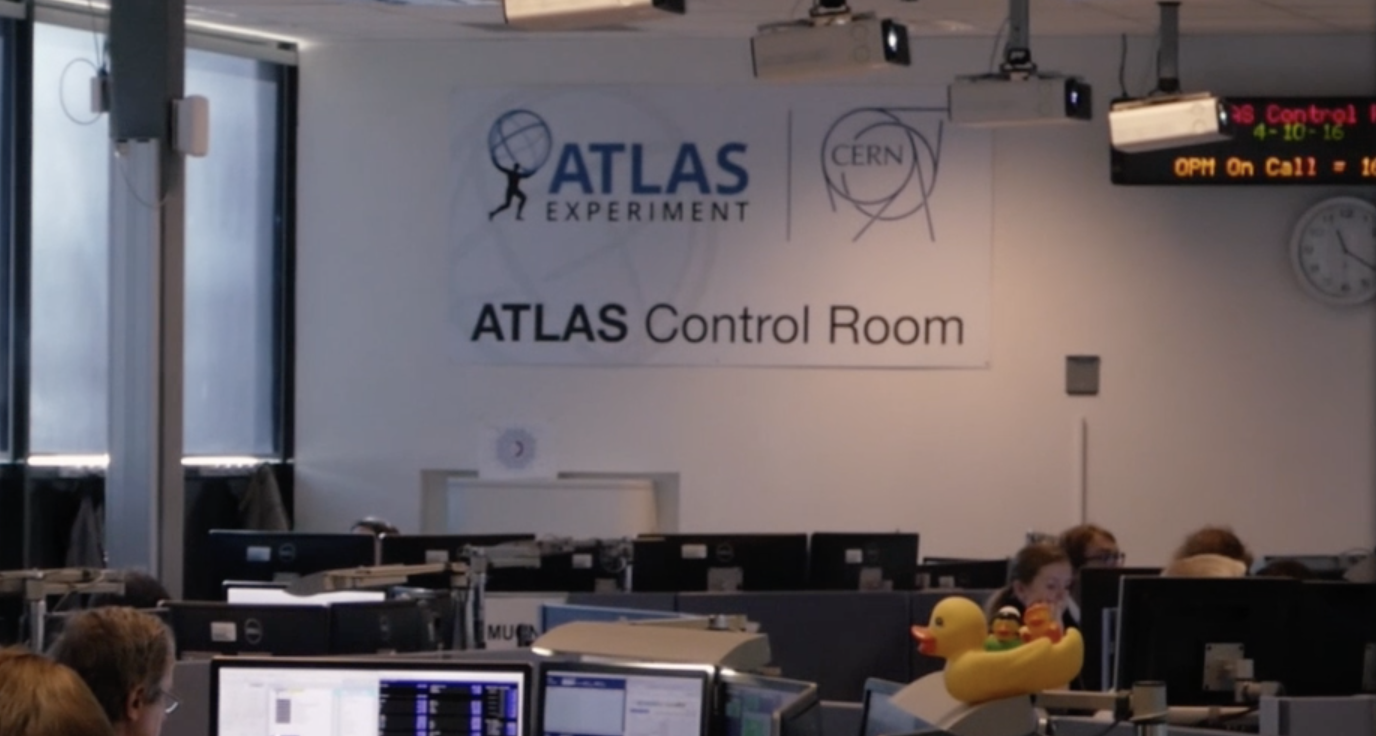
\includegraphics[width=\linewidth]{P1_pics/Titelbild.png}
\vspace{-.2cm}

\rule{12cm}{1pt} \\\vspace{-.6cm} \rule{10cm}{1pt}
\end{center}



\begin{abstract}
	In this report we analyze data taken at the ATLAS experiment located at the LHC. We study graphical representations of particle scattering events (event displays) using the especially for this purpose designed software ATLANTIS which is also used at ATLAS. After having studied event displays we move on and try to improve the calibration of the detector modules using a \texttt{C} program. Our final goal is to estimate the mass of the massive gauge boson $W^\pm$ using the technique of \textsc{Jacobi} peak determination. We use Monte Carlo simulations to further improve our results and study systematic error sources.
\end{abstract}
\begin{center}
	\rule{10cm}{1pt} \\\vspace{-.6cm} \rule{12cm}{1pt}
\end{center}

\setcounter{page}{-1}
\newpage

\tableofcontents
\thispagestyle{empty}
\newpage
\section{Introduction}
At the nuclear research center CERN in Geneva, Switzerland, several experiments are installed with the quest of searching for new fundamental physics and confirming up to this point in time available theories. With the LHC (\textbf{L}arge \textbf{H}adron \textbf{C}ollider) proton-antiproton collisions are studied at center of mass energies of \SI{14}{\tera\eV} \cite{manual}. In this experiment we will analyze data taken from ATLAS (\textbf{A} \textbf{T}oroidal \textbf{L}HC \textbf{A}pparatu\textbf{S}) detector. In order to do so we introduce the theory behind our analysis in section \ref{sec:theo}, then the experimental setup is described in detail in section \ref{sec:exp}. Armed with this we present the procedure of measurements and analysis in section \ref{sec:anal}; first we are going to study graphical event-displays of several events that have been recorded with the ATLAS detector in order to study the behavior of different particles in the detector. In a next step we will improve the calibration of the detector modules using $Z^0$ boson decays into electron-positron pairs. The main part of the analysis will then be to estimate the mass of the $W$ boson and thoroughly investigate systematic errors we collect with our specific methods. We finally draw conclusions from our findings in section \ref{sec:conc}.

\section{Theory}
\label{sec:theo}
In this section we will give the necessary theoretical fundamentals on which we  base our measurements and analysis. First the Standard Model of Particle Physics (SM) is briefly recapitulated, then production and decay of the heavy vector bosons $W^{\pm}$ and $Z^0$ are discussed along with their respective general properties. In a further step relativistic kinematics, especially regarding the analysis of $W$ and $Z$ decays at the LHC are explained in detail in addition with details regarding the detection of elementary particles.
\subsection{The Standard Model of Particle Physics}
The SM groups elementary particles into \emph{fermions} (spin $1/2$), which consist of \emph{quarks} and \emph{leptons}, and \emph{bosons} (spin $1$). On the particle physics scale there are three fundamental forces which are mediated by their respective gauge boson: 
\begin{enumerate}
	\item electromagnetic force, mediated by massless photons $\gamma$
	\item strong force, mediated by massless gluons $g$
	\item weak force, mediated by the massive $W^\pm, Z^0$ - bosons
\end{enumerate}
While only Quarks and gluons interact strongly every electrically charged particle interacts electromagnetically and all particles interact weakly. Responsible for the masses of $W^\pm, Z^0$ - bosons is the \textsc{Higgs}-mechanism. The last degree of freedom of this theory is embodied in a free particle, the \textsc{Higgs}-boson. 

A summary of the SM can be found in figure \ref{fig:sm}. \cite{povh}

\begin{figure}[htbp]
	\centering
	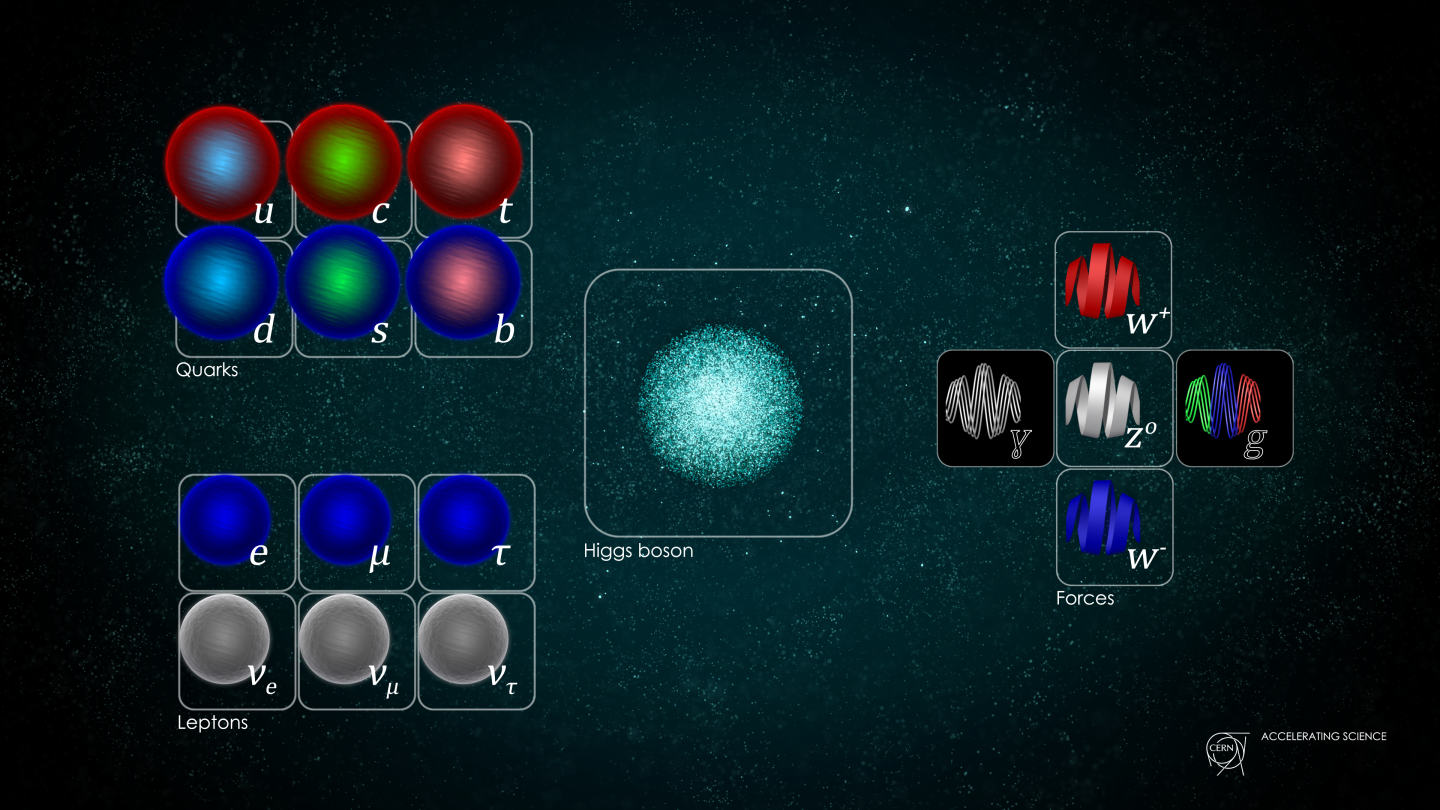
\includegraphics[width=.8\linewidth]{schematics/sm}
	\caption{Standard Model of Particle Physics, taken from \cite{sm}}
	\label{fig:sm}
\end{figure}
\newpage
\subsection{The heavy vector bosons $W^{\pm},Z^0$}
In this subsection the production/decay as well as general properties of $W/Z$ bosons are discussed.
\subsubsection{Production and decay}
When in the process of colliding two particles a sufficiently high center of mass (CMS) energy is achieved, \emph{real} $W/Z$ bosons can be created. The most important production processes in proton-antiproton collisions are sketched as \textsc{Feynman} diagrams in figure \ref{fig:feyn}. It is important to note that only parts (partons) of each proton collide, therefore not the CMS energy of the proton-collision needs to exceed the boson mass but the CMS energy in the system of the colliding partons, which is also called \emph{hard system}. \cite{manual}
\begin{figure}[htbp]
	\centering
\feynmandiagram [horizontal=a to b] {
		i1[particle=$q$] -- [fermion] a -- [fermion] i2 [particle=$\overline{q'}$],
		a -- [scalar, edge label=$W/Z$] b,
		b,
	};
\feynmandiagram[vertical=a to b]{
	i1 [particle=$q$]--[fermion] a-- [scalar] f1 [particle=$W/Z$], 
	a -- [fermion] b-- [gluon] f2 [particle=$g$],
	i2 [particle=$\overline{q'}$]-- [anti fermion] b
	
};
\feynmandiagram[vertical=a to b]{
i1 [particle=$q$]--[fermion] a, 
a-- [scalar] f1 [particle=$W/Z$],
a -- [fermion] b,
i2 [particle=$q'$]-- [anti fermion] b,
b-- [gluon] f2 [particle=$g$]
};
	\caption{Processes which contribute to $W/Z$-production, in the case of $Z$ production, $q'=q$}
	\label{fig:feyn}
\end{figure}
The lifetime of $W/Z$ bosons is not long enough as to measure them directly, therefore one has to identify their respective decay products. The $W$ boson decays as 
\begin{align*}
	W^\pm & \to q \overline{q'} && \text{BR } \sim 2/3 \\
	& \to l \overline{\nu_l} && \text{BR } \sim 1/3,
\end{align*}

into quarks and leptons and the $Z$ boson decays as
\begin{align*}
	Z^0 & \to q \overline{q} & \text{BR } \sim 70\% \\
	& \to \nu_l \overline{\nu_l} & \text{BR } \sim 20\%\\
	&\to l\bar{l} & \text{BR } \sim 10\% 
\end{align*}
into quarks leptons (excluding $\tau$ because it is too heavy) and neutrinos of all families.
\cite{pdg}
\subsubsection{General properties}
Currently the in table \ref{tab:key} following key properties of the heavy gauge bosons are recognized by the Particle Data Group (PDG) \cite{pdg}.
\begin{table}[htbp]
	\centering
\begin{tabular}{c|cc}

	& $W^\pm$ & $Z^0$  \\
	\hline
	mass / GeV &  $80.379 \pm 0.012$   & $91.1876\pm 0.0021$  \\
	
	el. charge / $e$ & $\pm 1$  & 0 \\
	
	spin / $\hbar$& 1 & 1 \\
	
\end{tabular}
\caption{Key parameters of $W/Z$ boson}
\label{tab:key}
\end{table}
One can directly see that the $W$-mass is not estimated as well as the $Z$-mass. This is due to the harder detectable decay channels of the $W$ boson. 

\subsection{Detection of elementary particles}
In principle charged leptons (especially electrons) are detected quite easily since they interact with matter by being slowed down, emitting bremsstrahlung photons which in turn interact with matter via \emph{photoelectric effect, \textsc{Compton}-scattering} and \emph{pair creation}, creating what is called an electromagnetic shower. It is obvious that primary photons are thus also detectable easily. Quarks do not exist as free particles and will soon after production begin hadronizing, resulting in a strongly boosted bunch of hadrons, which is called a \emph{jet}. Gluons are also observed as jets. Hadrons can interact with matter via inelastic scattering and ionization ultimately forming what is then analogously called a hadronic shower. The size of any shower is proportional to the deposited energy which can be read out using scintillators. Neutrinos do scarcely interact with matter at all and are thus very difficult to detect. To the ATLAS detector they are invincible. \cite{manual}

\subsection{Decay kinematics}
Let us consider the general two body decay of some particle $X$. We can then calculate the invariant mass of said particle if the 4-momenta of the decay products $p_i,i=1,2$ have been measured $$m_X=\sqrt{(p_1+p_2)^2}.$$ If we observe the decay many times the invariant mass will follow a \textsc{Breit-Wigner} distribution from which the true value and the decay width can be obtained \cite{manual}. This method works well for the decay $Z^0\to e^+e^-$ but not for the decay $W^-\to e^-\overline{\nu_e}$ since the neutrino is invisible to the detector. One would have to rely on indirect measurements of the neutrino momentum. Thus, to estimate the $W$ mass we exploit the fact that the distribution of the transverse momentum $p_t$ should feature a sharp peak at half the $W$ mass and no events after it if we look at a head on symmetric (net momentum vanishes) collision with a two body decay \cite{povh} 

\begin{equation}
	\frac{\d\sigma}{\d p_t}\propto\frac{1}{\sqrt{\frac{1}{4}M_W^2-p_t^2}}.
\end{equation}
The peak is called \textsc{Jacobi} peak. In reality the peak will be smeared because of detector resolution, non-zero transverse momentum of the $W$ boson and its finite decay width \cite{manual}. The $W/Z$ bosons can gain non-zero transverse momenta if gluons are emitted during the production, see figure \ref{fig:feyn}.

\subsection{Pre lab questions I}
We will answer here the first mandatory pre lab questions given in the manual \cite{manual}.
\subsubsection*{Question A: Decay of a $\boldmath Z^0$ boson}
\indent \emph{Which value does the momentum of an electron have in the decay $Z^0\to e^+e^-$ if the $Z^0$ is at rest?}

If the $Z^0$ is initially at rest the net momentum of electron and positron has to vanish, $\mathbf{p}_-=-\mathbf{p}_+$. We have also $E_++E_-=M_Z$ and since we can neglect the electron masses at this energies we find $E\approx|\mathbf{p}|=\frac{M_Z}{2}$. 
\subsubsection*{Question B: Scattering reaction $\boldmath e^+e^-\to\tau^+\tau^-$}

\indent \emph{How large is the momentum of tau leptons in the reaction $\boldmath e^+e^-\to\tau^+\tau^-$, if the reaction takes place in the center-of-mass system at $\sqrt{s}=\SI{5}{\giga\eV}$}?

Starting from 4-momentum conservation $$\begin{pmatrix}
	\sqrt{s} \\
	0
\end{pmatrix}=\begin{pmatrix}
E_-\\
\mathbf{p}_-
\end{pmatrix} +\begin{pmatrix}
E_+\\
\mathbf{p}_+
\end{pmatrix} $$
and squaring we find with $|\mathbf{p}_-|=|\mathbf{p}_+|=|\mathbf{p}|$  $$s=4(|\mathbf{p}|^2+m_e^2) \Leftrightarrow |\mathbf{p}| = \sqrt{\frac{s}{4}-m_\tau}=\SI{2.12}{\giga\eV}.$$
The tau mass was taken from the PDG \cite{pdg}.
\newpage
\section{Experimental Setup -- The ATLAS detector}
\label{sec:exp}
Since our budget was limited and the pandemic is still around, we couldn't take our own datasets at CERN and relied on given datasets. %This section will give an overview over the ATLAS detector.

The ATLAS detector is one of multiple detectors at the nuclear research center CERN in Geneva. Via the LHC -- a circular collider -- hadrons get accelerated and collide in the detector. Since the LHC is a symmetric collider, the center of mass system is also the laboratory system, for which the resulting center of mass Energy for a proton-proton pair can be up to $E_{CM}=14$ TeV. \cite{manual}   

This section will give insight in the functionality and structure of the ATLAS detector. A cross section of the detector is depicted in figure \ref{fig:ATLAS}. The detector consists of three detection Layers \cite{manual}:
\begin{enumerate}
	\item \textbf{Inner detector:} The inner detector is responsible for reproducing the trajectory of produced particles. It consists out of a Pixel Detector with about 80 million pixels, a Semiconductor tracker (SCT) and a Transition Radiation Detector (TRT) out of thin gas drift chambers. Around the inner detector is a solenoid magnet with a magnetic field of about $B_{\text{ATLAS}}=2T$.  
	\item \textbf{Calorimeters:} The inner detector is surrounded by two calorimeters. The first calorimeter is the electromagnetic calorimeter (ECAL) which detects the energy of light leptons by producing and detecting electromagnetic showers. The other calorimeter is the hadron calorimeter (HCAL) which does the same for the hadrons (and hadron showers). The HCAL consists of iron and is a thick layer to absorb all hadrons completely.
	\item \textbf{Myon chambers:} Because the detector material is for Myons highly penetrable. Myons leave traces in the chambers. The chambers have their own toroid magnet, with which independent momentum measurements can be done.
\end{enumerate}
In a cartesian coordinate system, the $z$-axes of the detector is parallel to the beam direction.\\
The transverse momentum 
\begin{equation*}
	p_t=\sqrt{p_x^2+p_y^2}
\end{equation*}
 is an often used quantity together with the rapidity 
$$y=\frac{1}{2}\ln\left({\frac{E+p_z}{E-p_z}}\right)\Rightarrow y_{\text{hard}}=\frac{1}{2}\ln\left({\frac{x_A}{x_B}}\right)$$
of an event to describe the properties of a detected particle or jet \cite{manual}.
If the invariant mass is zero, the rapidity for a system can be approximated by the so called pseudo-rapidity $\eta$ which can be written with the angle $\theta$\footnote{relative angle of the particle to the beam axis \cite{theta}} as:
$$\eta=-\ln\left(\tan\frac{\theta}{2}\right).$$
The range of $\eta$ varies for different kinds of particles. In ATLAS leptons can be detected at the range of $-2.5<\eta<2.5$ and hadrons at $-5<\eta< 5$ \cite{manual}. The advantage of the pseudo rapidity is, that it is  Lorentz invariant under longitudinal boosts \cite{theta}. Another important measurement is the azimuthal angle $\phi$. It is also invariant under the Lorentz boosts as the quantity $$\Delta R=\sqrt{(\Delta \eta)^2+(\Delta \phi)^2}$$ which defines a general distance dimension. Jet detection and reconstruction rely on $\Delta R$. For energy entries of a jet follows the rule $\Delta R<R_{\text{max}}=0.7$ measured in the $\eta \phi$ plane. In the following analysis only the transverse momentum $p_t$, the pseudo rapidity $\eta$ and the azimuthal angle $\phi$ will be used. \cite{manual} 
\begin{figure}
	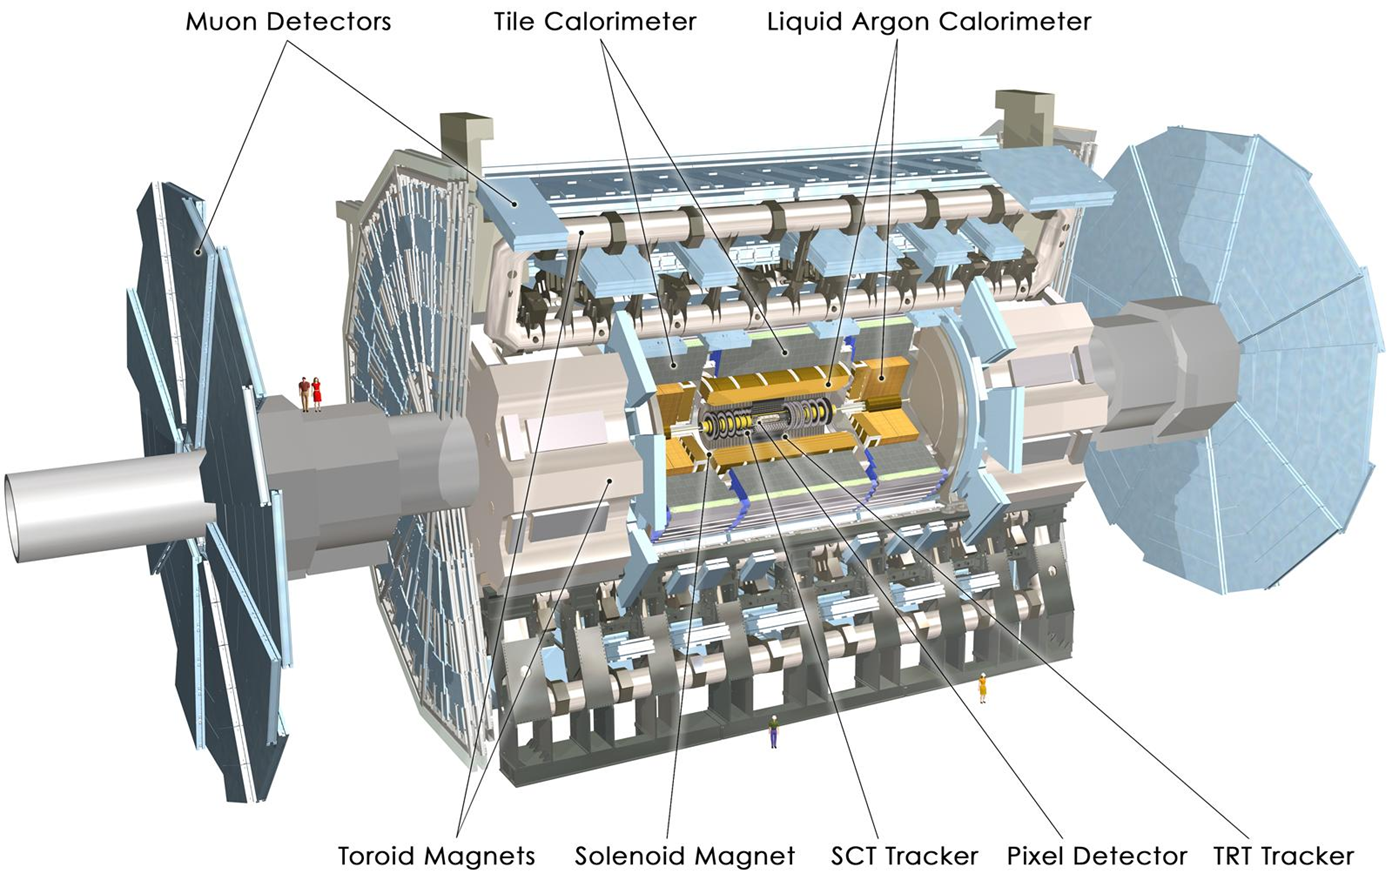
\includegraphics[width=\linewidth]{P1_pics/schematics/ATLAS.png}
	\caption{The ATLAS Detector \cite{ATLAS_detector}}\label{fig:ATLAS}
\end{figure}
\newpage
\section{Measurements and Analysis}
\label{sec:anal}
In the following we will explain our experimental procedure and directly draw conclusions in the form of our analysis.
\subsection{Part 1: Graphic Display of Particle Reactions}
First we make ourselves acquainted with the graphical representation of different events that have been recorded by ATLAS with the graphical event display ATLANTIS \cite{atlantis}. 
\subsubsection{General Investigation of Event Displays}
We load several pre-selected learning datasets containing only one type of reaction, for example single electrons or muons. We took screenshots of arbitrary (nice) events in the datasets and they are displayed in the following figures. The respective reaction is given in the caption. The ATLANTIS display features a cross section of the detector barrel region on the top left, a zoom in to the center of the detector on the top right and a sideways view of the detector on the bottom. The tracking system is displayed in black and hits therein are colored white. If a track has been reconstructed successfully it will be displayed as a blue line in the tracking region. After this the ECAL (green) and HCAL (red) follow. The muon detectors are the blue outliers. Energy deposits are indicated as yellow.
%\newpage
\begin{figure}[H]
	\centering
	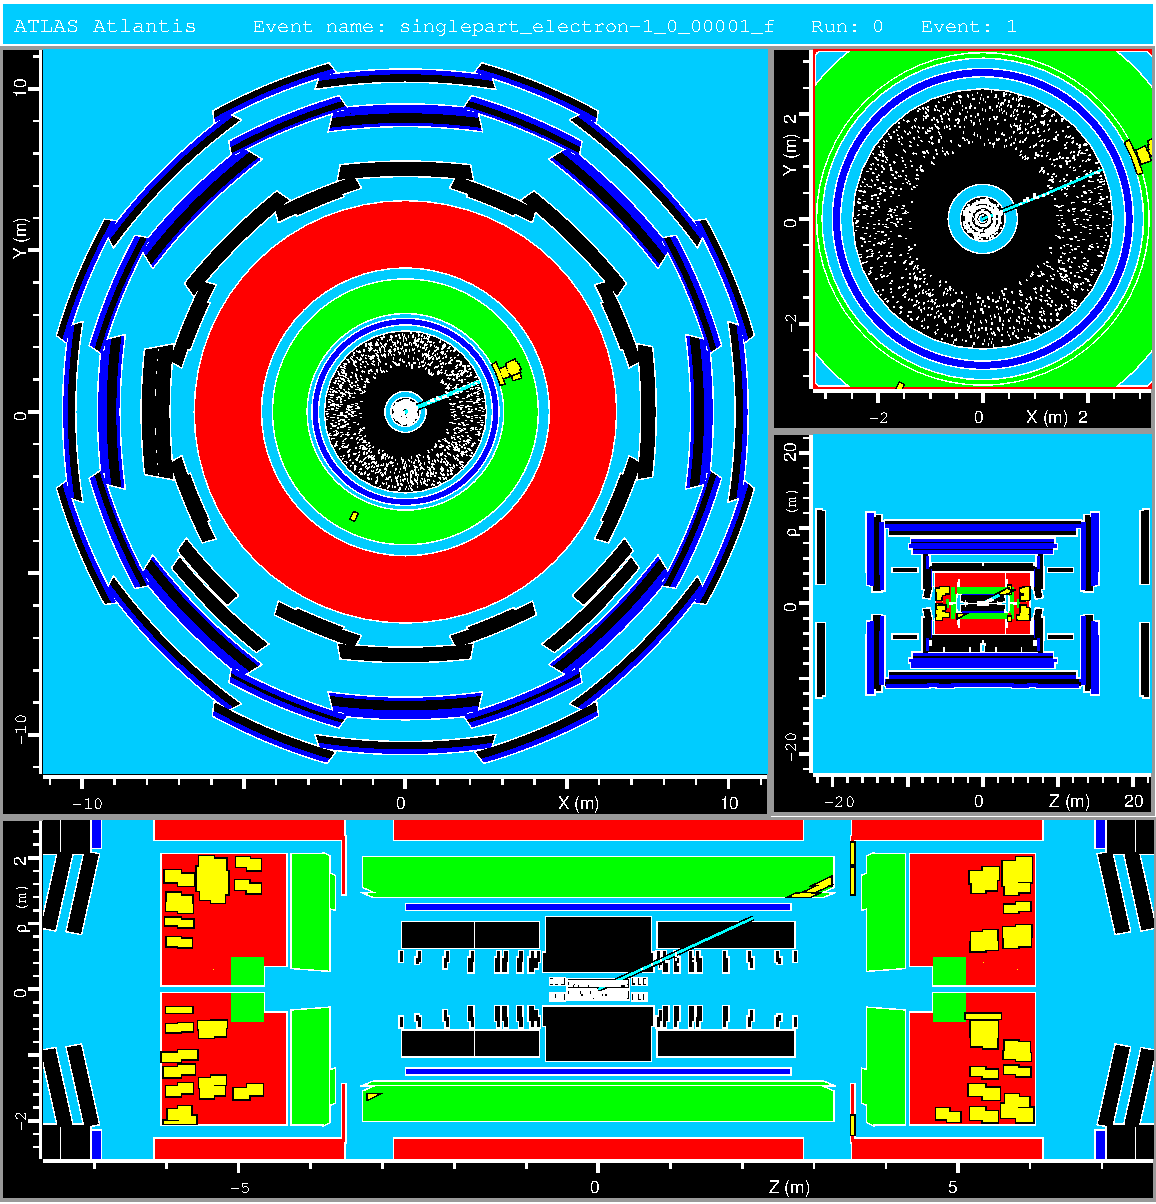
\includegraphics[width=.8\linewidth]{atlantis/electron_training}
	\caption{Event from the electron learning dataset.}
\end{figure} 
The electron is charged and leaves a clear path in the tracking system. It deposits significant energy in the ECAL as would be expected in the form of an electromagnetic shower. We recognize that there are several small energy deposits rather than one big.

\begin{figure}[H]
	\centering
	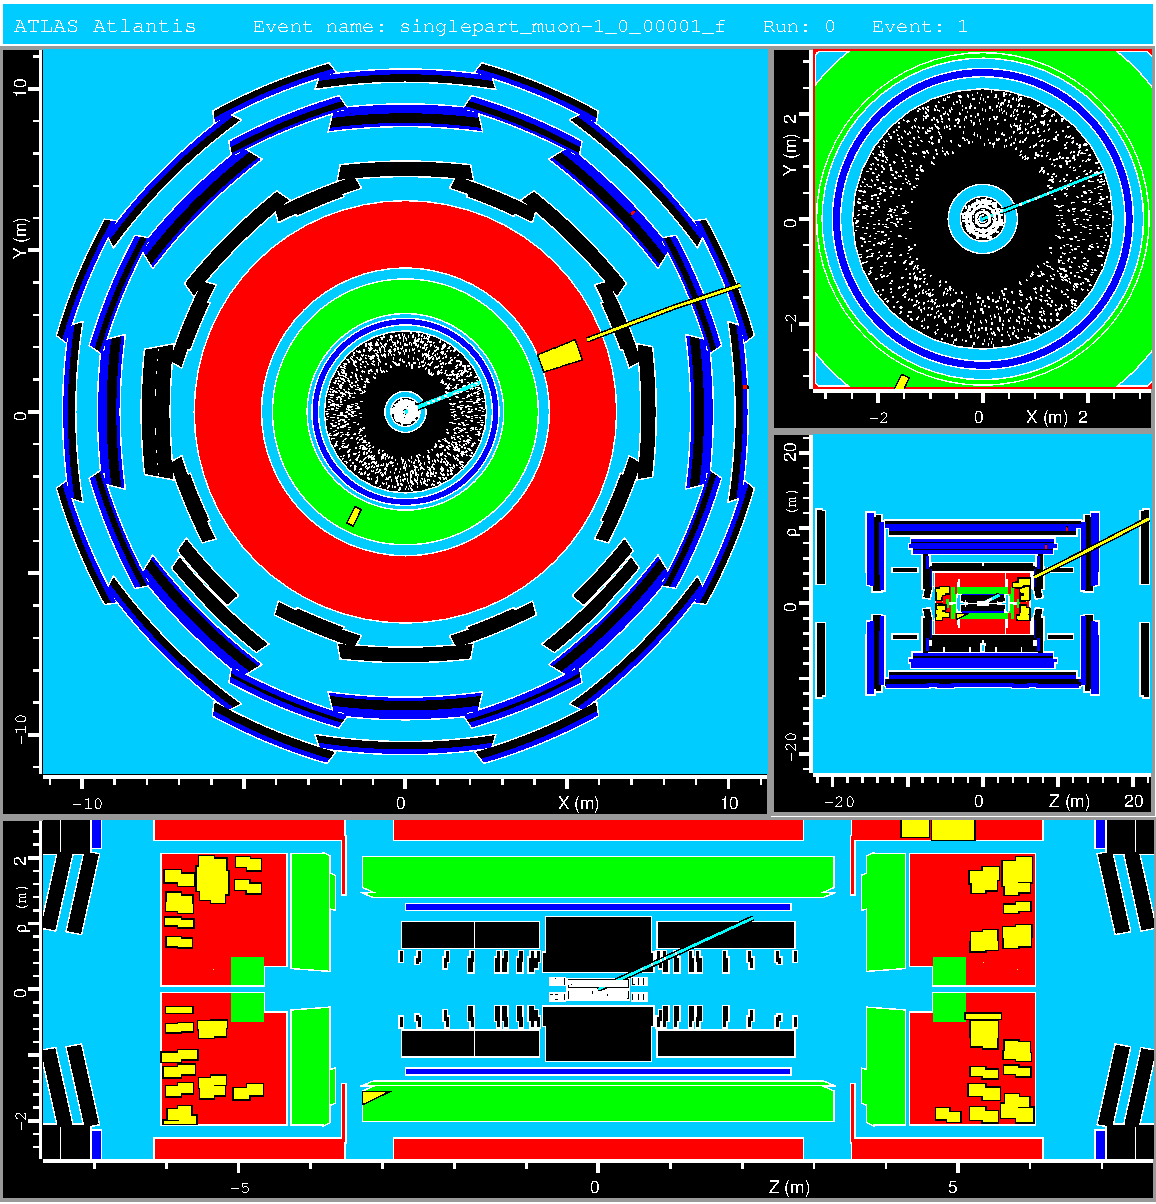
\includegraphics[width=.8\linewidth]{atlantis/muon_testing}
	\caption{Event from the muon learning dataset.}
\end{figure} 
If we look at a muon event we see that it does in fact not deposit any energy in the ECAL. This can be explained by its high mass which hinders it from inducing an electromagnetic shower. The muon does then interact somewhat with the HCAL and again leaves a track in the muon tracking chambers. Since the HCAL employs iron to trigger bremsstrahlung photons it is possible that a shower has been formed, although it must be very low energetic since the track of the muon is hardly changed. 

\begin{figure}[H]
	\centering
	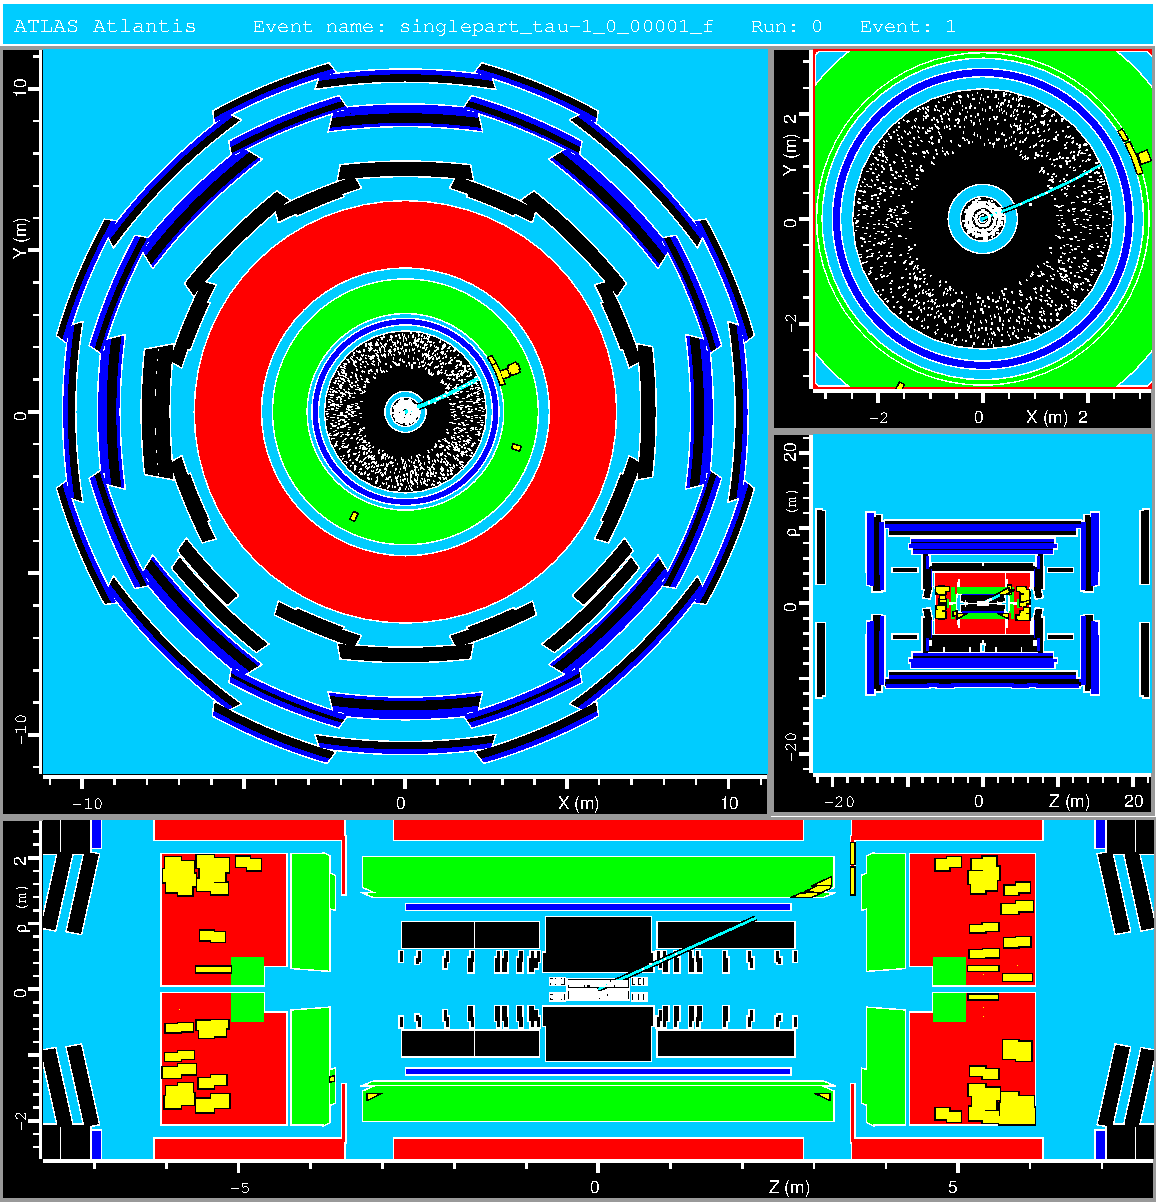
\includegraphics[width=.8\linewidth]{atlantis/tau_testing}
	\caption{Event from the tau learning dataset.}
\end{figure} 
With its very short life time of $c\tau_\tau\approx \SI{90}{\micro\m}$ the detector will not see the tau directly but its decay products. Since there is significant energy deposit in the ECAL and a clearly visible track it is likely that the decay $$\tau\to e\overline{\nu_e}$$ is observed here with the neutrino being invisible to the detector.

\begin{figure}[H]
	\centering
	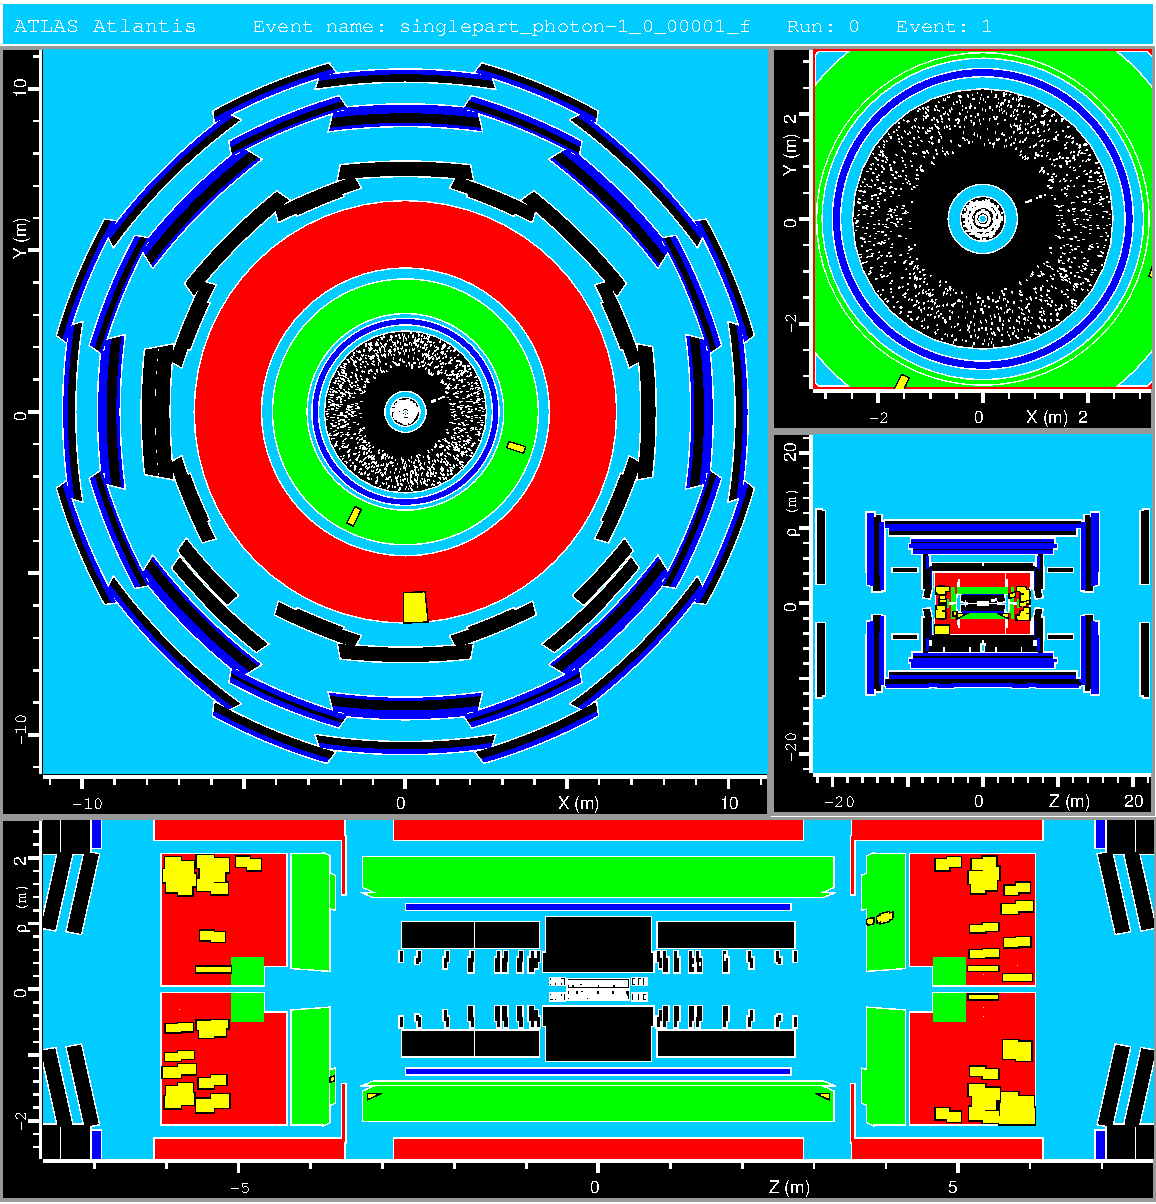
\includegraphics[width=.8\linewidth]{atlantis/photon_testing}
	\caption{Event from the photon learning dataset.}
\end{figure} 
If we observe a photon all we can see is an energy deposit in the ECAL since the photon is not charged and will thus not leave an observable track.

\begin{figure}[H]
	\centering
	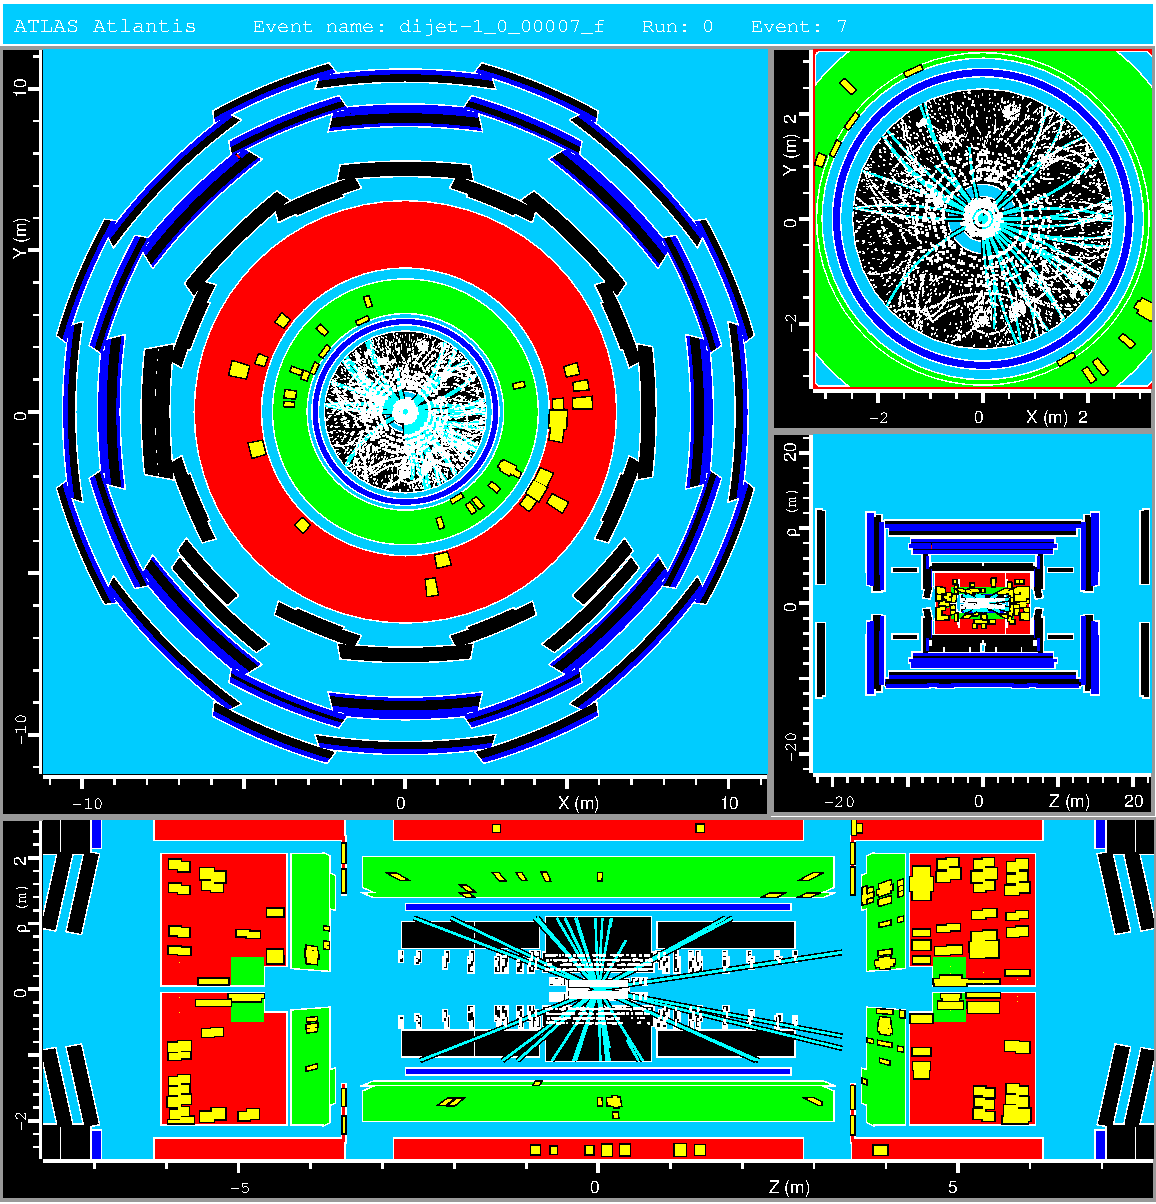
\includegraphics[width=.8\linewidth]{atlantis/dijet_testing}
	\caption{Event from the two jet learning dataset.}
\end{figure} 
Jets are also clearly recognizable while looking at the respective event display; There are energy deposits in ECAL and HCAL in roughly two directions. Many charged particles leave a track and induce hadronic showers in the HCAL. By just looking at it no further conclusions with respect to the particles that took part in this particular reaction can be drawn.
\subsubsection{Assignment 1 -- Energy and momentum measurements}
We loaded again the electron dataset and measured energy and momentum of 20 electrons. We then calculated the ratio $\beta=\frac{p}{E}$. The results are in table \ref{tab:resbeta} and figure \ref{fig:resbeta}. One would expect the majority of events featuring a $\beta\approx 1$. However we observe that this majority is slightly shifted towards values greater than one. This of course is unphysical, since $\beta=v/c$, which means that the energy is estimated as too small or the momentum too big at this point.
\begin{table}[htbp]
	\centering
	\begin{tabular}{c|c|c|c}
		Event No. & $p$ / GeV & $E$ / GeV & $\beta$  \\
		\hline
		1         & 26.20          & 54.7                & 0.479 \\
		2         & 22.78          & 35.2                & 0.647 \\
		3         & 7.55           & 56.6                & 0.133 \\
		4         & 129.82         & 162.3               & 0.800 \\
		5         & 3.27           & 47.7                & 0.069 \\
		6         & 79.01          & 66.2                & 1.194 \\
		7         & 95.93          & 78.7                & 1.219 \\
		8         & 37.40          & 30.6                & 1.222 \\
		9         & 89.35          & 85.9                & 1.040 \\
		10        & 235.24         & 242.3               & 0.971 \\
		11        & 105.14         & 105.3               & 0.998 \\
		12        & 28.62          & 28.1                & 1.019 \\
		13        & 53.41          & 46.4                & 1.151 \\
		14        & 32.92          & 64.3                & 0.512 \\
		15        & 105.64         & 80.8                & 1.307 \\
		16        & 93.52          & 82.1                & 1.139 \\
		17        & 113.98         & 92.7                & 1.230 \\
		18        & 155.35         & 283.0               & 0.549 \\
		19        & 36.4           & 33.8                & 1.077 \\
		20        & 55.46          & 48.8                & 1.136
	\end{tabular}
\caption{Results of energy and momentum measurements}
\label{tab:resbeta}
\end{table}
\begin{figure}
	\centering
	\includegraphics[width=\linewidth]{plots/beta_histo}
	\caption{Histogram of the above results}
	\label{fig:resbeta}
\end{figure}

\subsubsection{Assignment 2 -- Decay of $Z$ boson}
As a next step we measure energy and momentum of three possible electron positron pairs which originated from the decay of a $Z$ boson. For this we load the especially suited dataset which contains $Z^0\to e^+e^-$ candidates. We chose for our measurements pairs of opposite charge and momentum which energies roughly added up to the mass of the $Z$ boson. The three events chosen by us are depicted in figure \ref{fig:zee}.

\begin{figure}[htbp]
	\centering
	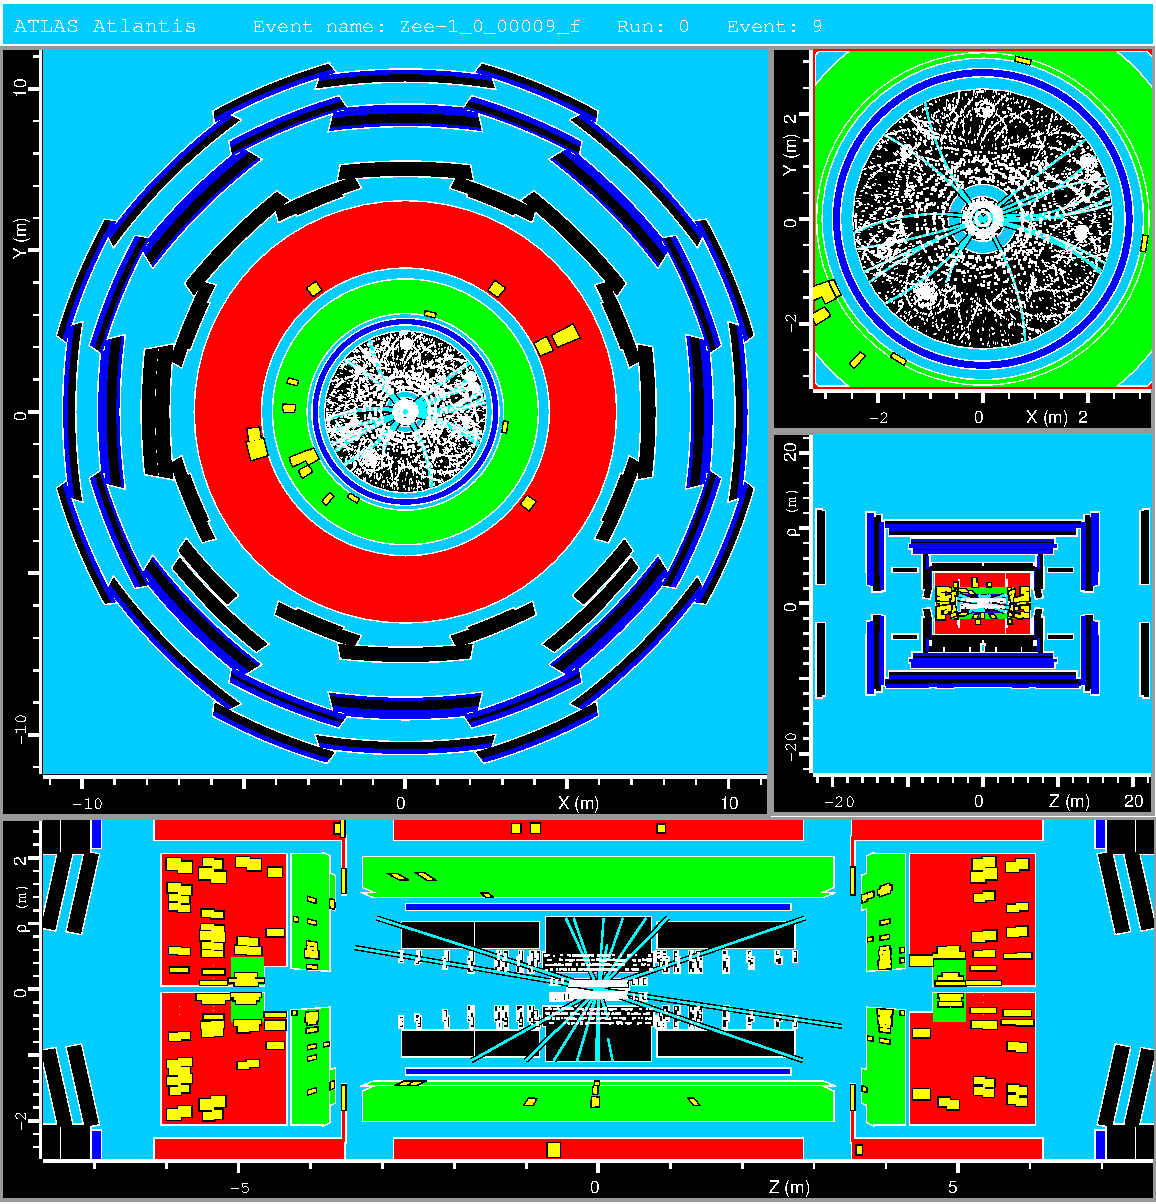
\includegraphics[width=.32\linewidth]{atlantis/zee_1}
	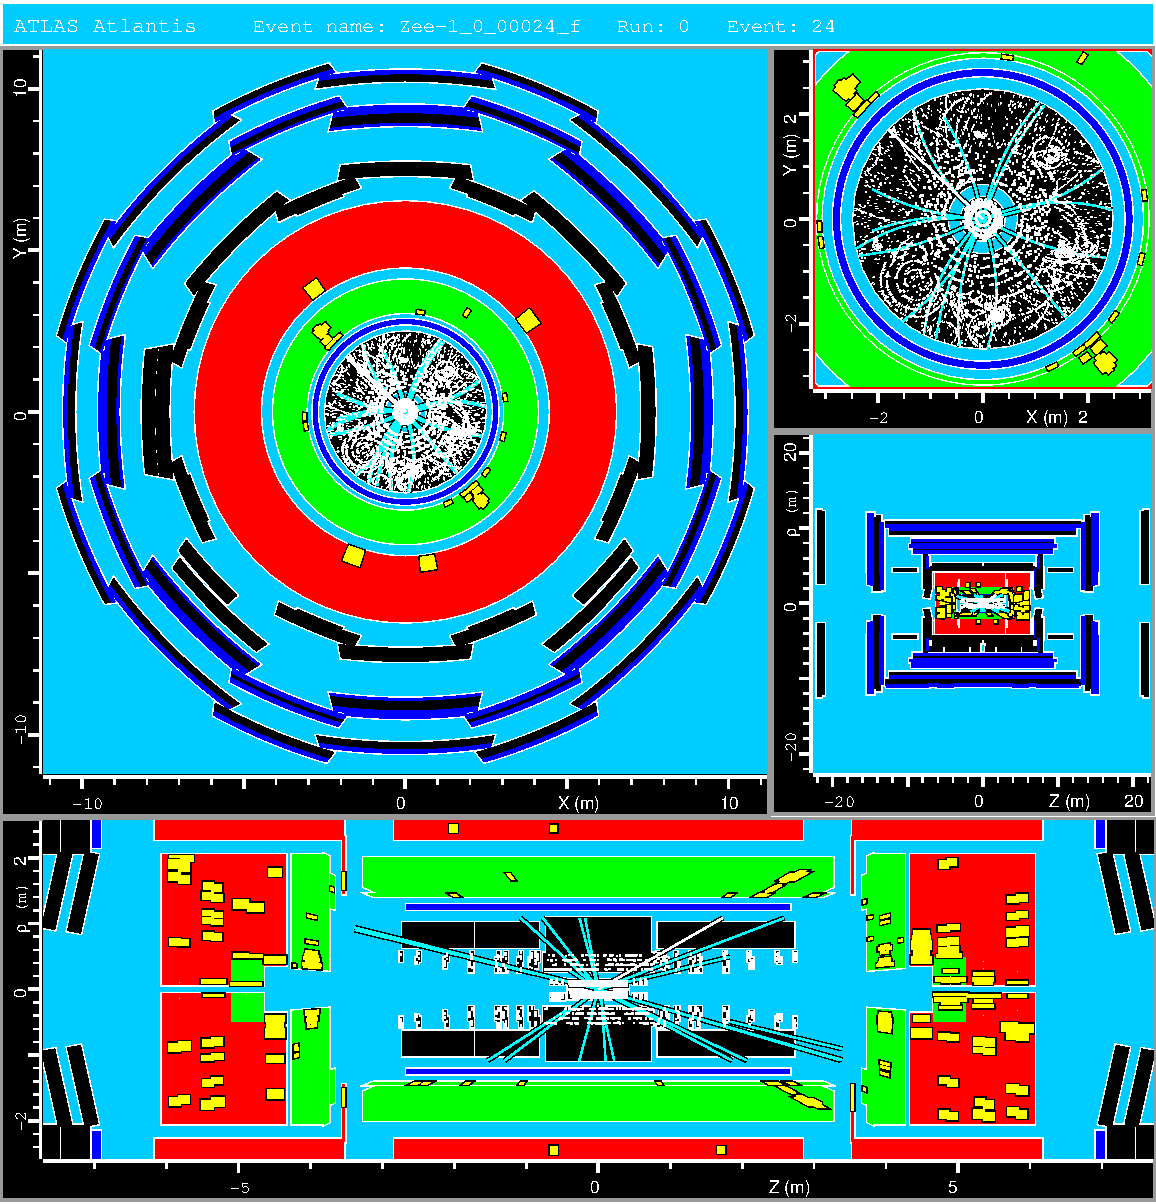
\includegraphics[width=.32\linewidth]{atlantis/zee_2}
	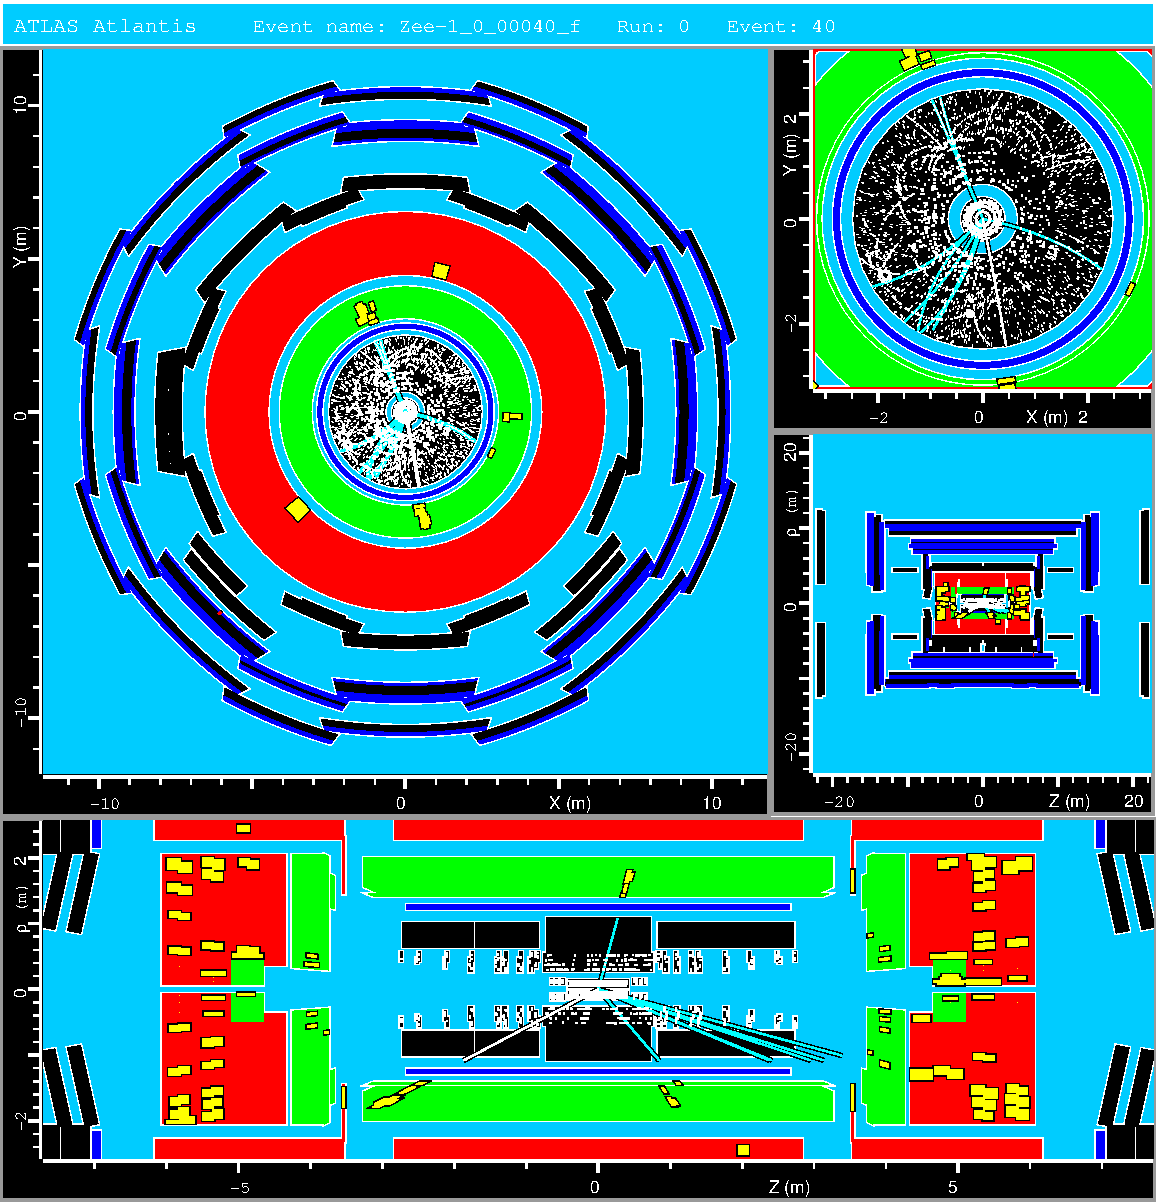
\includegraphics[width=.32\linewidth]{atlantis/zee_3}
	\caption{possible $Z\to e^+e^-$ events}
	\label{fig:zee}
\end{figure}

We wish to determine the invariant mass of electron and positron. It is given by \begin{align}
	\label{eq:zmass}
	\begin{split}
			(p_1+p_2)^2=2m_e^2+2p_1\cdot p_2&=2m_e^2+2E_1E_2-2|\mathbf{p}_1||\mathbf{p}_2|\cos\theta\\&\approx 2E_1E_2(1-\cos\theta)=4E_1E_2\sin^2\frac{\theta}{2}
	\end{split}
\end{align}
We therefore measured Energy and momentum as well es the azimuthal angle $\phi$ and the polar angle $\theta$ via the pseudo-rapidity $\eta$. Our results are in table \ref{tab:reszee}.
\begin{table}[htbp]
	\resizebox{\linewidth}{!}{%
	\begin{tabular}{c|c|c|c|c|c|c|c|c|c|c|c}
		Event &  $|\mathbf{p}_1|$/ GeV & $\eta_1$ & $\theta_1$          & $\phi_1$ /deg & $|\mathbf{p}_2|$/ GeV & $\eta_2$  & $\theta_2$           & $\phi_2 /deg$   & $E_1$ / GeV & $E_2$ / GeV & $M_{12}$ / GeV \\
		\hline
		1     & 6.38             & 2.488   & 0.165 & 230.592 & 5.46            & -2.373 & 2.955  & 11.154  & 48.3           & 30.2           & 78.47     \\
		2     & 69.77            & 1.247   & 0.559 & 136.157 & 61.97           & 1.308  & 0.528 & 310.645 & 68             & 61.8           & 35.41     \\
		3     & 35.28            & 0.246   & 1.327  & 112.598 & 50.26           & -1.315 & 2.617  & 281.188 & 41.2           & 29.8           & 59.12    
	\end{tabular}
}
\caption{Results of invariant mass}
\label{tab:reszee}
\end{table} 

The momenta were reconstructed as $$\mathbf{p}=|\mathbf{p}|\cdot
\begin{pmatrix}
\cos\phi\sin\theta\\
\sin\phi\sin\theta\\
\cos\theta	
\end{pmatrix}.$$
Unfortunately we are not able to reproduce the $Z$ mass even remotely. This can only be due to faulty measurements: Either we have not measured electron and positron but some other particles or we determined the energy wrong by not taking the whole cluster into account. Since we had to make our decision on which particles to measure and what region to take into account for the energy measurement by eyeballing the event display it is thus possible to choose wrong, which we did.
\subsection{Part 2: Calibration of Electrons}
After we have made ourselves familiar with event displays it is now our goal to further improve the calibration of the various detector modules which can at this point deliver different signals for the same amount of energy input depending on detector region. Typically the detected energy will be smaller than the real energy because the particles have lost some energy that was not detectable \cite{manual}. We will use the decay $Z^0\to e^+e^-$ and determine the invariant mass of the electron positron pair. It should deliver us the $Z$ mass of $m_Z=\SI{91.1876\pm0.0021}{\giga\eV}$ \cite{pdg} which is a well known parameter and therefore suited for use as calibration reference. We load the real ATLAS data set with $Z\to e^+e^-$ candidates for this purpose. We estimate the invariant mass by fitting a \textsc{Voigt} function \cite{voigt} and a background function to the histogram which contains the invariant mass. The \textsc{Voigt} function is the convolution of a \textsc{Gaussian} with a \textsc{Breit-Wigner} distribution. This is done because smearing effects like the finite detector resolution have to be taken into account \cite{manual}. The fit also gives an estimate of the detector resolution (smearing effects due to systematic errors) via the width of the \textsc{Gaussian} \cite{manual}.
\subsubsection{Initial plots of decay signals}
First we created histograms of electron and positron energy as well as their invariant mass, which is computed as in eq. \eqref{eq:zmass} (without the approximation $m_e\approx 0$). The results are in figure \ref{fig:hist_ini}.

\begin{figure}[htbp]
	\centering
	\begin{subfigure}{.49\linewidth}
		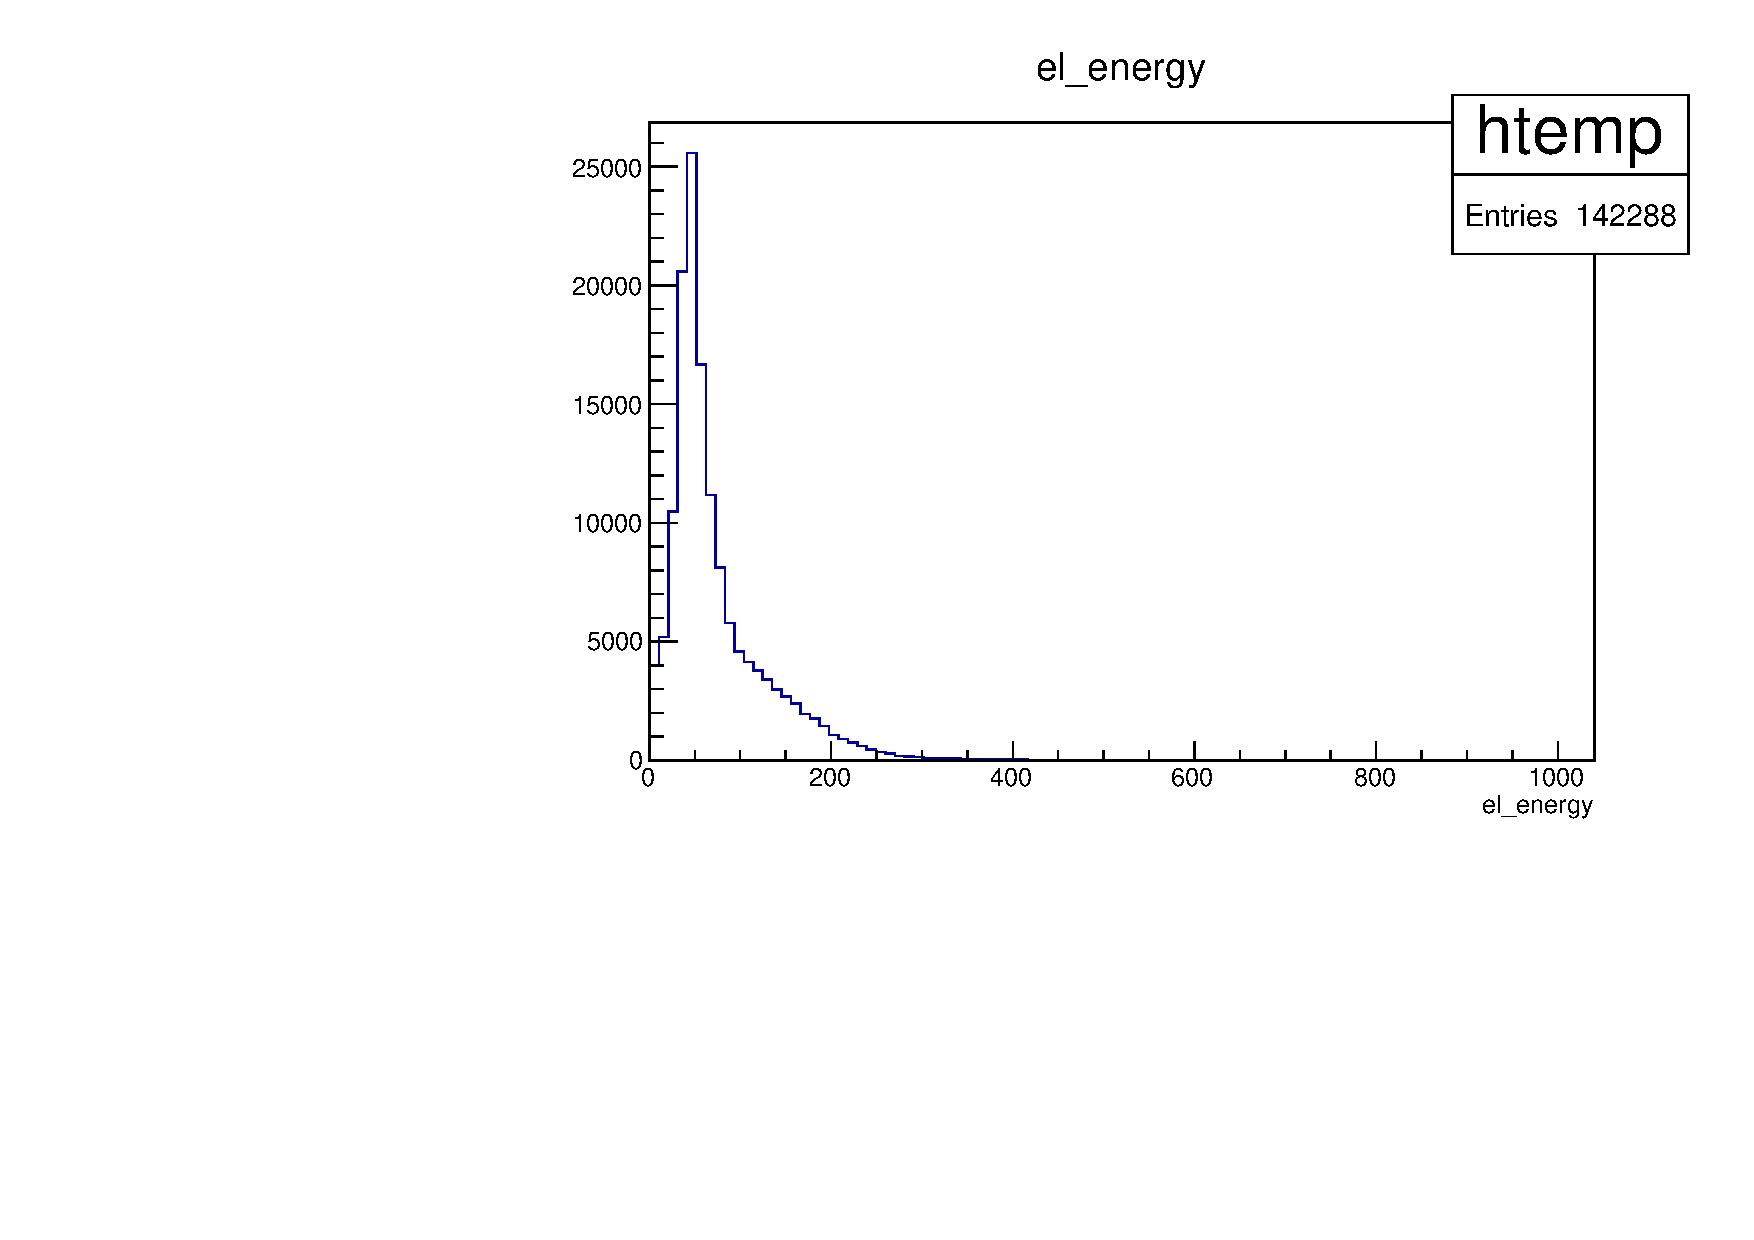
\includegraphics[width=\linewidth]{calibration/el_energy}
		\subcaption{Electron energy, x-axis: energy/ GeV, y-axis: counts}
	\end{subfigure}
\begin{subfigure}{.49\linewidth}
	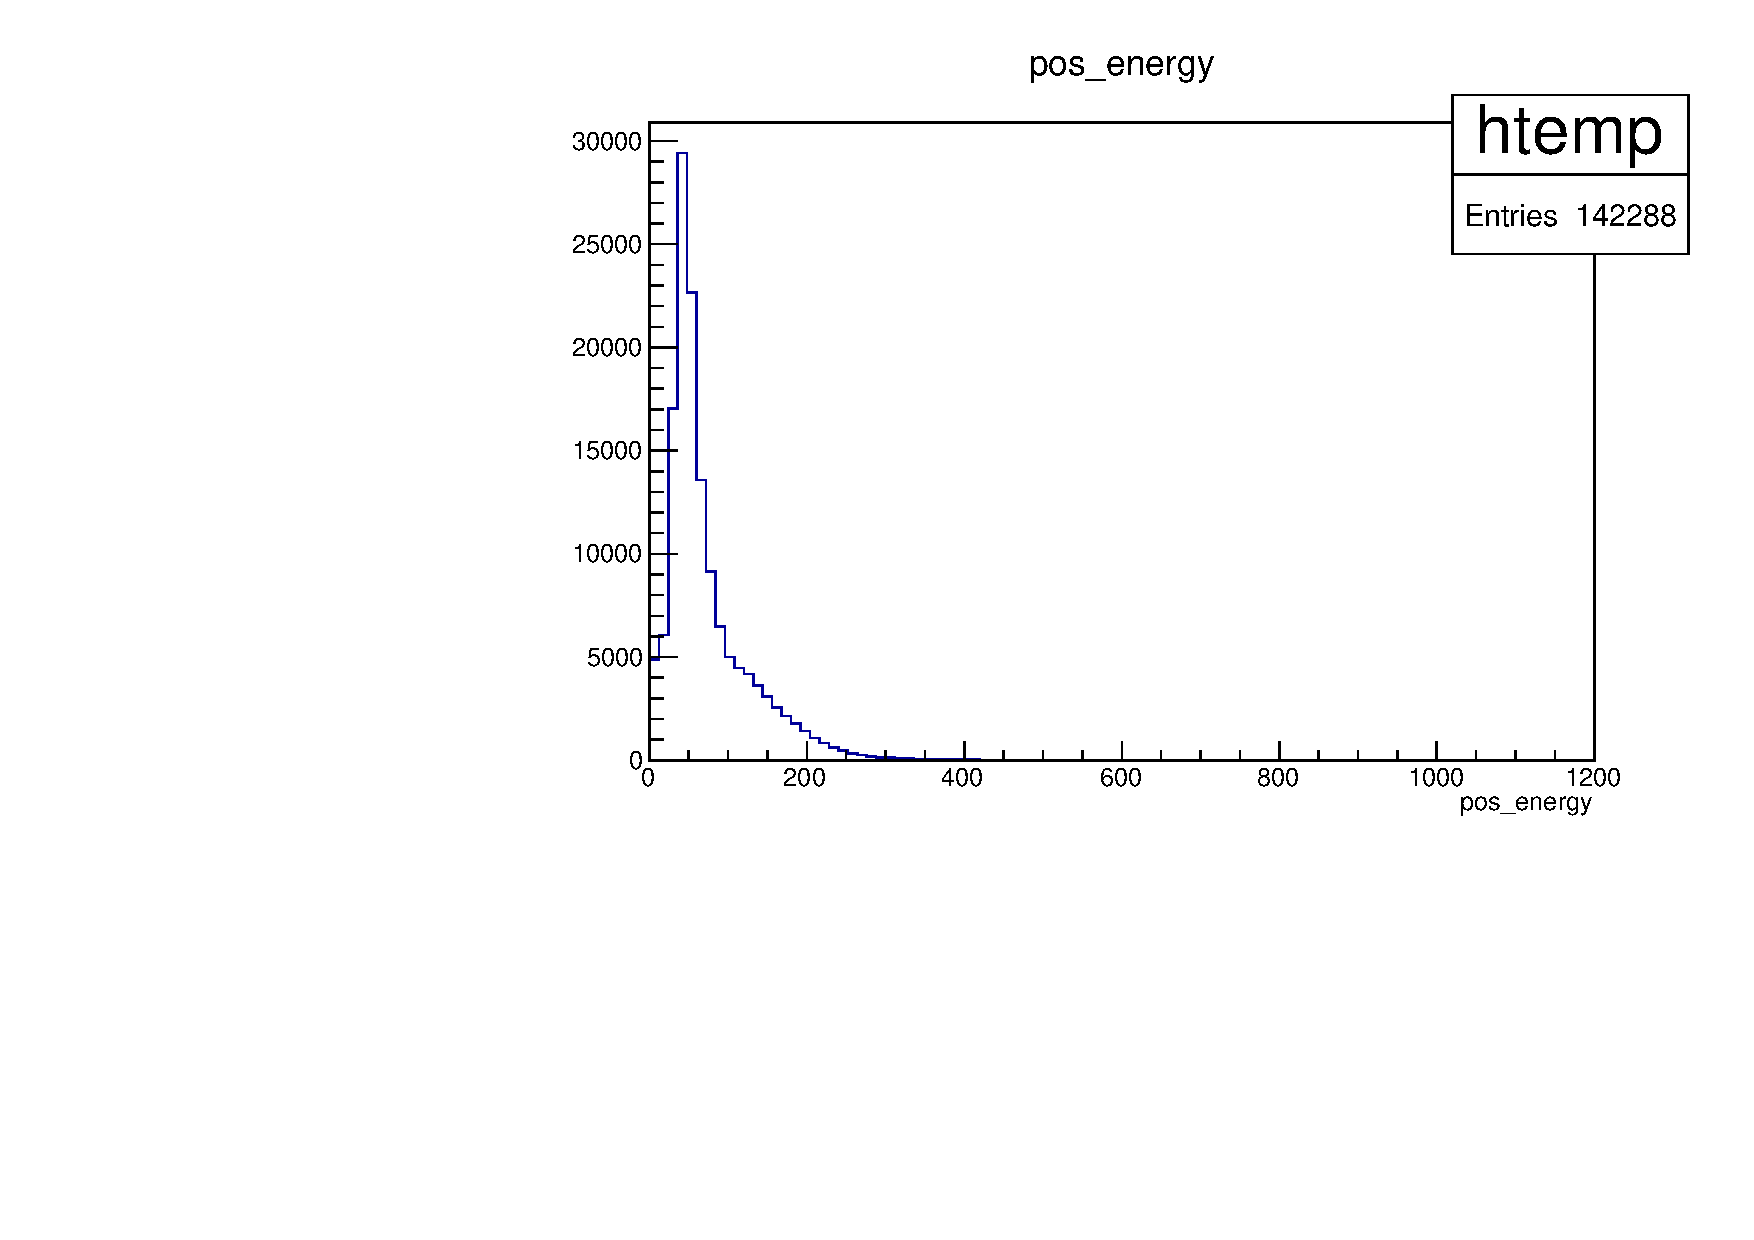
\includegraphics[width=\linewidth]{calibration/pos_energy}
	\subcaption{Positron energy, x-axis: energy/ GeV, y-axis: counts}
\end{subfigure}
\begin{subfigure}{.8\linewidth}
	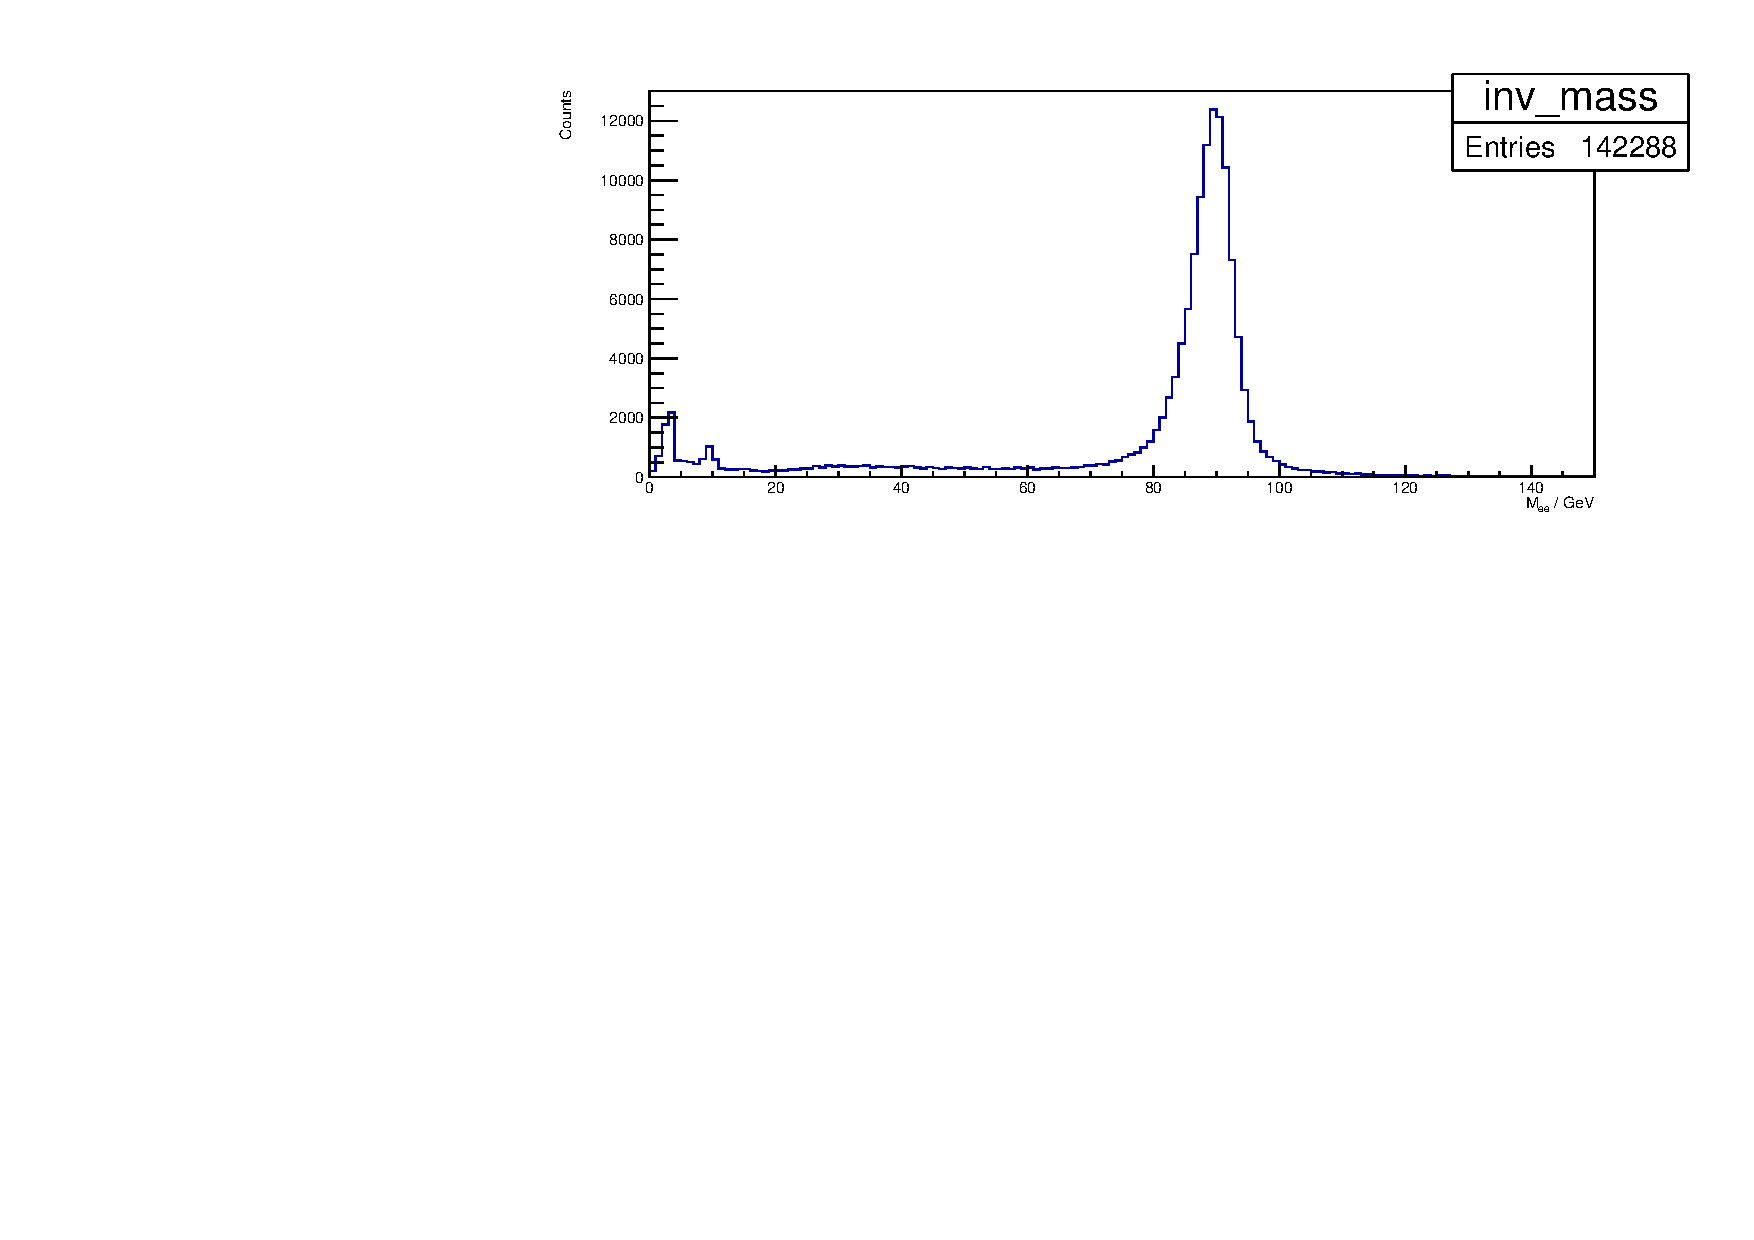
\includegraphics[width=\linewidth]{calibration/inv_mass}
	\subcaption{Invariant mass}
\end{subfigure}
\caption{Initial histograms of decay parameters}
\label{fig:hist_ini}
\end{figure}
We see that the electron/positron energy distribution is roughly the same which they should be as their kinematic properties are the same save the charge. One can actually observe that the distributions features a \textsc{Jacobi} peak because we are looking at a two body decay here. The invariant mass distribution is mostly centered around roughly the $Z$ mass. We obviously expect this from a two body decay originating from a $Z^0$. However one can also see small peaks around masses of less than \SI{20}{\giga\eV}. Either particles with this respective masses have been created and the respective electrons misidentified as $Z^0$ decay candidates or one/both particles have been misidentified as electrons. In any case do this cases not form a significant contribution to the whole spectrum if compared to the $m_Z$ peak. 
\subsubsection{Constructing a calibration function}
Since a fit to the invariant mass peak of the electron-positron pairs does not yield the correct $Z$ mass yet (see figure \ref{fig:calib}), we want to further improve the calibration of the detector. The improved calibration can be applied by us through the \texttt{C} file \texttt{ElecCalib.C}. It can be accessed in our \href{https://github.com/krausejm/advanced_lab_course}{GitHub repository} and also in the appendix \ref{sec:Appendix}. We wish to apply a function which corrects the detected energy $E_\text{raw}$ based on the detector region to an adjusted value $E_\text{calib}=C\cdot E_\text{raw}$. As quantitative measure of detector region we use the transverse momentum $p_t$, the pseudo-rapidity $\eta$ and the azimuthal angle $\phi$. They directly correspond to spherical coordinates $$(r,\theta,\phi)\leftrightarrow(p_t,\eta,\phi),$$
since $\eta=-\ln\tan\theta$ and the (transverse) penetration depth into the detector of some particle will be proportional to its transverse momentum. We can thus write $$E_\text{calib}=C(p_t,\eta,\phi)\cdot E_\text{raw}.$$ We estimate the correction factor as $$C(p_t,\eta,\phi)=\frac{m_Z}{m_Z^\text{fit}(p_t,\eta,\phi)}$$ with the correct and well known Z mass $m_Z=\SI{91.1876}{\giga\eV}$ \cite{pdg} because the $Z^0$ mass mainly depends on electron or positron energy. Our strategy is now to estimate the correction factor for various detector regions $(p_t,\eta,\phi)$ using a separation ansatz $C(p_t,\eta,\phi)=C_p(p_t)C_\eta(\eta)C_\phi(\phi)$ by fitting the invariant mass peak using only events that correspond to a certain interval in $p_t,\eta$ or $\phi$ of the electron (this choice is arbitrary we could also use the positron). The order we chose was $$C(p_t,\eta,\phi)=1\to C_\eta(\eta)\to C_\eta(\eta)C_\phi(\phi)\to C_\eta(\eta)C_\phi(\phi)C_p(p_t).$$ In principle one could do this iteratively but we already got a good estimate of the correct mass for the whole detector after the first iteration and further attempts of improving the result resulted in worsening the outcome. We divided each coordinate into the following intervals
\begin{align*}
	\eta&\in\{[-2.5,-2.4),[-2.4,-2.3),\dots[2.5)\}\\
	\phi&\in\{(,-\pi],\left[-\frac{11}{12}\pi,-\frac{10}{12}\pi\right),\dots\left[\frac{11}{12}\pi,\right)\}\\
	p_t&\in\{(,\SI{15}{\giga\eV}),[\SI{15}{\giga\eV},\SI{20}{\giga\eV}),\dots[\SI{80}{\giga\eV},)\}.
\end{align*}    

\begin{figure}[t]
	\centering
	\begin{subfigure}{.49\linewidth}
		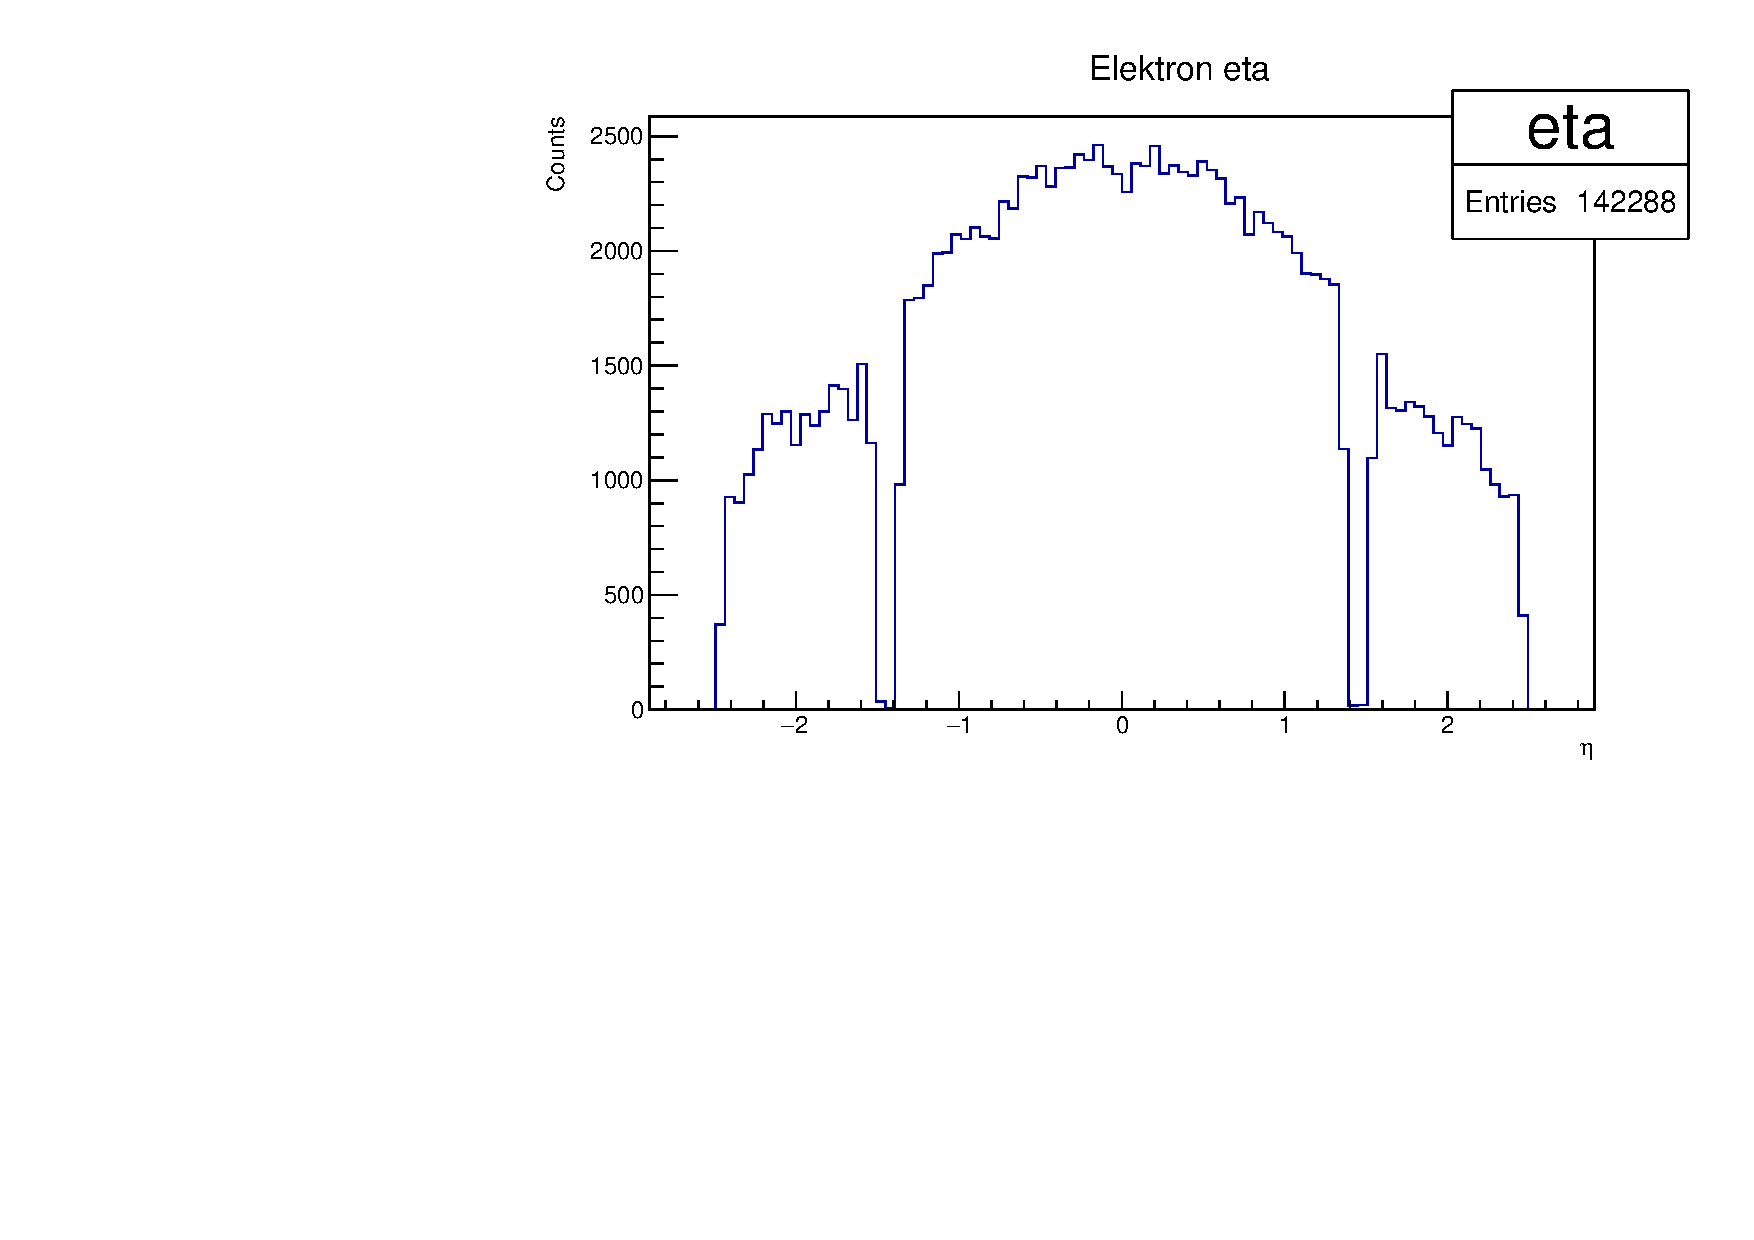
\includegraphics[width=\linewidth]{calibration/el_eta_full}
		\subcaption{}
	\end{subfigure}
	\begin{subfigure}{.49\linewidth}
		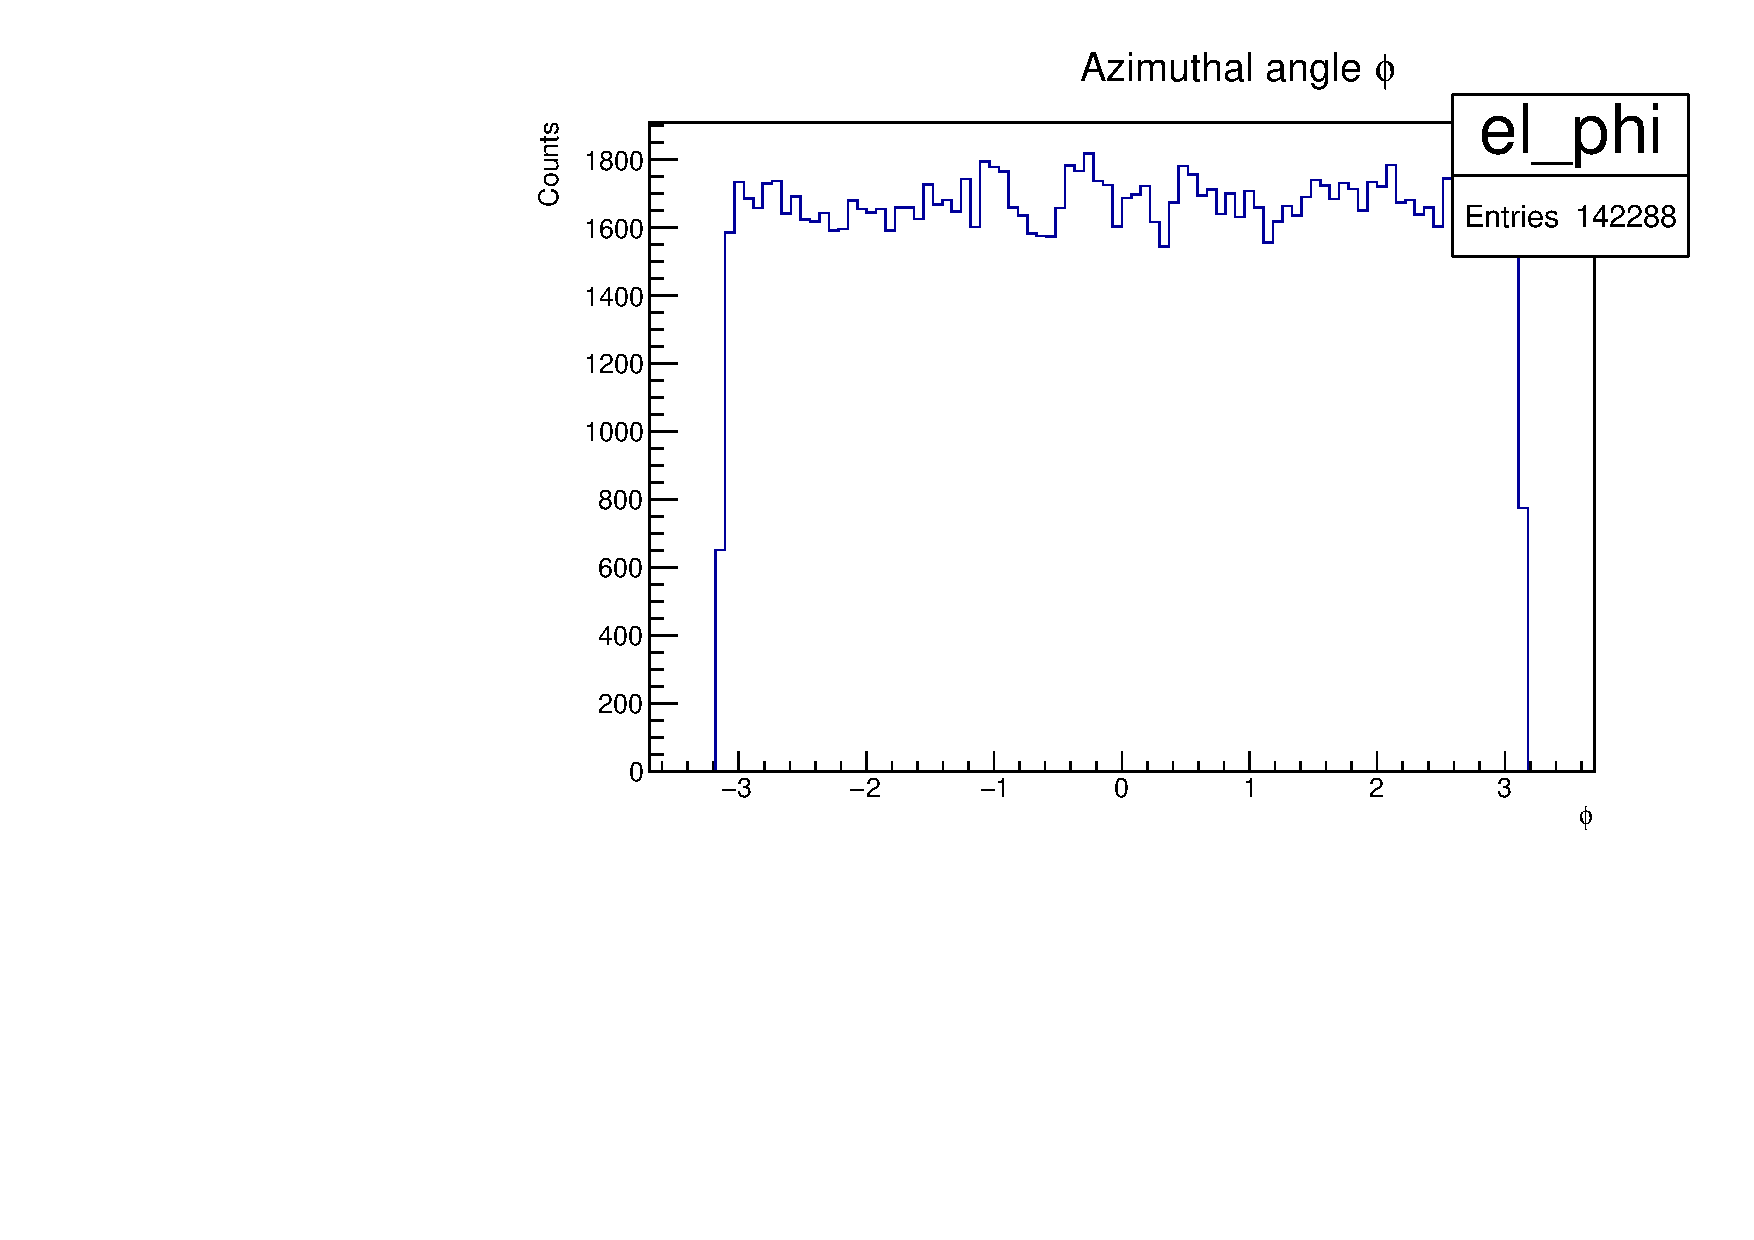
\includegraphics[width=\linewidth]{calibration/el_phi_full}
		\subcaption{}
	\end{subfigure}
	\begin{subfigure}{.49\linewidth}
		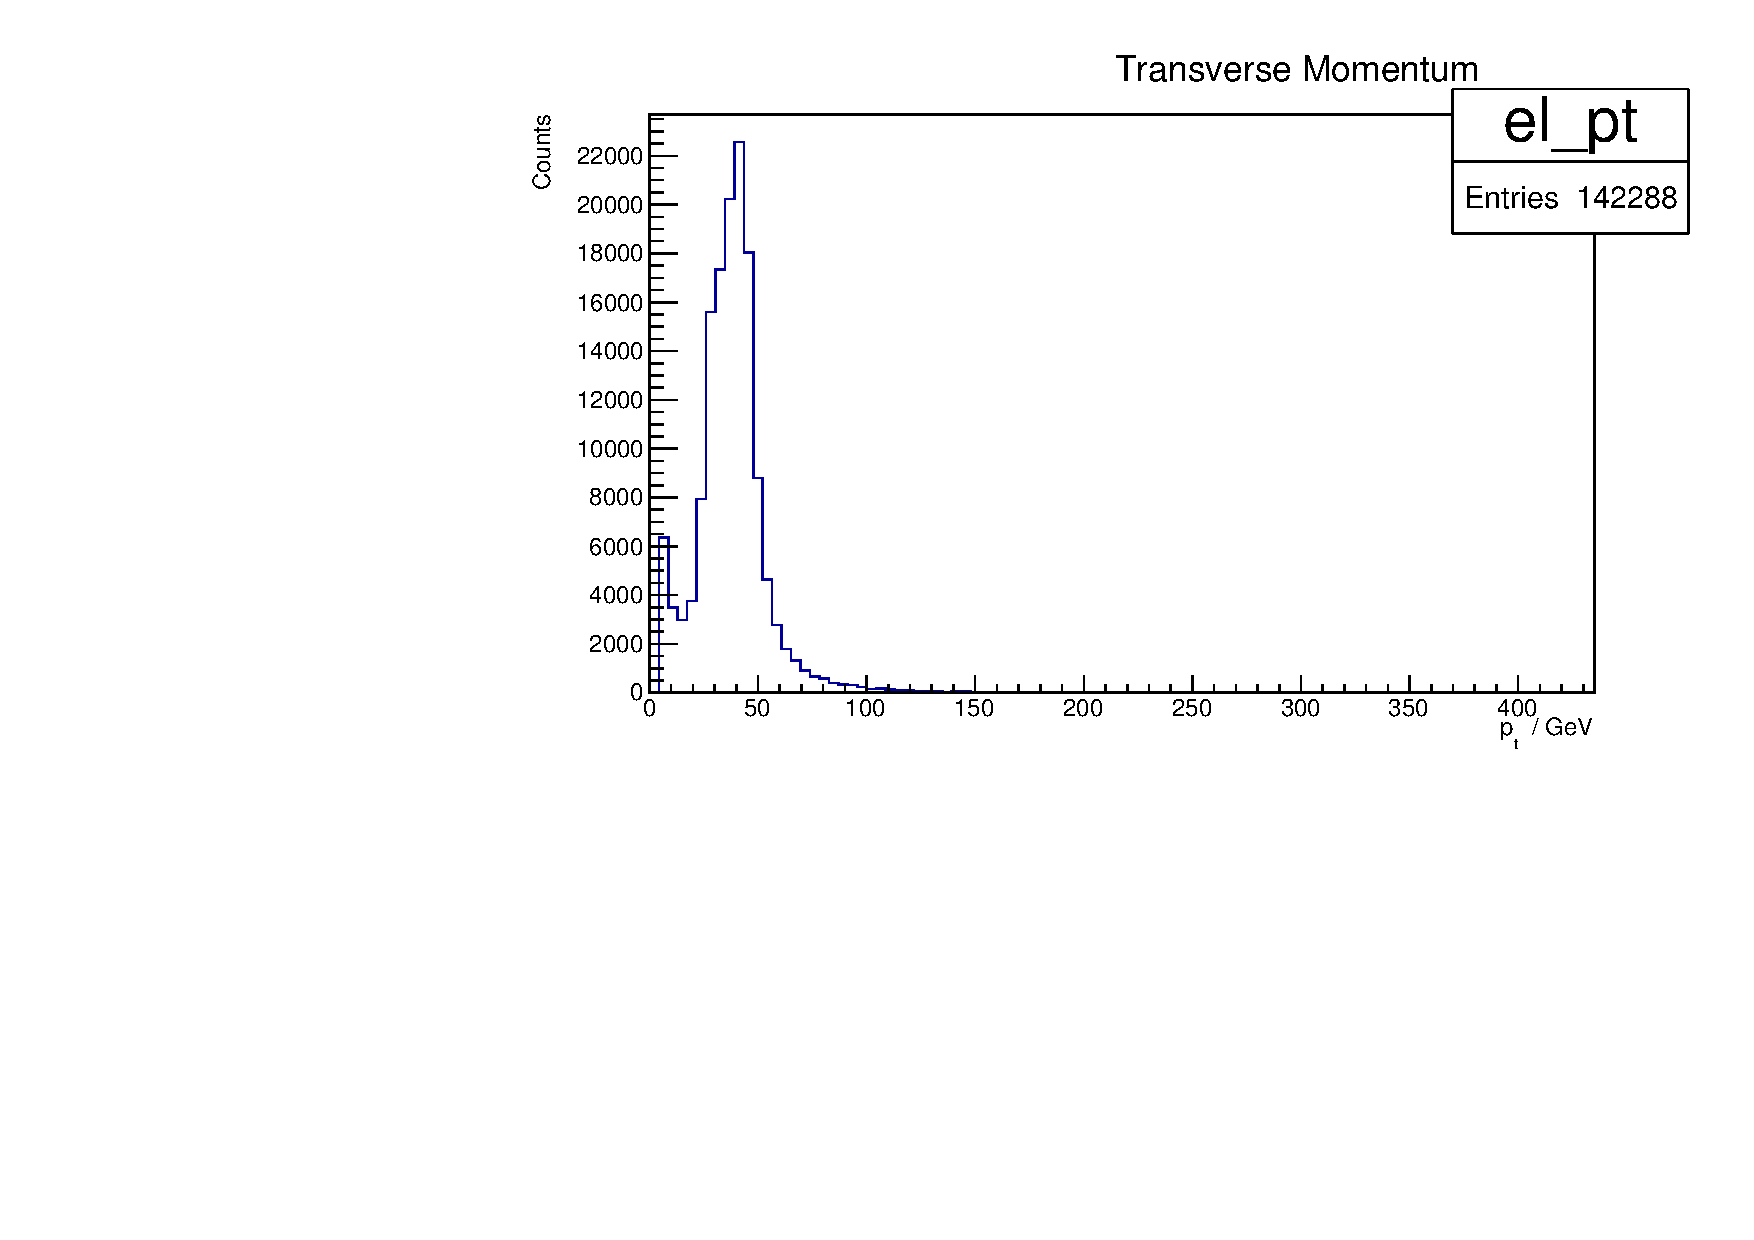
\includegraphics[width=\linewidth]{calibration/el_pt_full}
		\subcaption{}
	\end{subfigure}
	\caption{Spectra of the detector coordinates}
	\label{fig:etaphip}
\end{figure}

That means $\frac{1}{10}$ steps in $\eta$, $\frac{\pi}{12}$ steps in $\phi$ and \SI{5}{\giga\eV} steps in $p_t$. We made this decisions based on the spectra of each of the mentioned variables which are shown in figure \ref{fig:etaphip}.

Since the amount of events is roughly constant over the different angle regions, we decided it to be reasonable choosing equidistant binning in those variables, which allowed enough events to fit the invariant mass peak confidently. The transverse momentum distribution features very many events from roughly \SIrange{20}{80}{\giga\eV} and few out of these bounds. For this reason the binning is finer inside the mentioned interval than outside.

\textbf{Remark:} Inspecting the $\eta$ spectrum one sees that $\eta\in[-2.5,2.5]$ as expected \cite{manual} and that there are almost no events for $|\eta|\approx 1.4$. The reason for this is the detector geometry which does not allow detection in this region \cite{Collaboration_2008}.

Figure \ref{fig:calib} shows the result of our calibration. We were able progress from \begin{align*}
	m_Z^{\text{raw}}=\SI{89.47\pm0.02}{\giga\eV} && \Delta^\text{raw}=\SI{2.446\pm0.025}{\giga\eV}
\end{align*}
to 
\begin{align*}
	m_Z^{\text{calib}}=\SI{91.22\pm0.02}{\giga\eV} && \Delta^\text{calib}=\SI{2.281\pm0.024}{\giga\eV},
\end{align*}
with the detector resolution $\Delta$. Having now established an improvement in detector resolution and estimated $Z^0$ mass which only deviates in a $2\sigma$ interval from the literature value we are ready to proceed with the main part of our analysis.
\begin{figure}[htbp]
	\begin{subfigure}{.49\linewidth}
		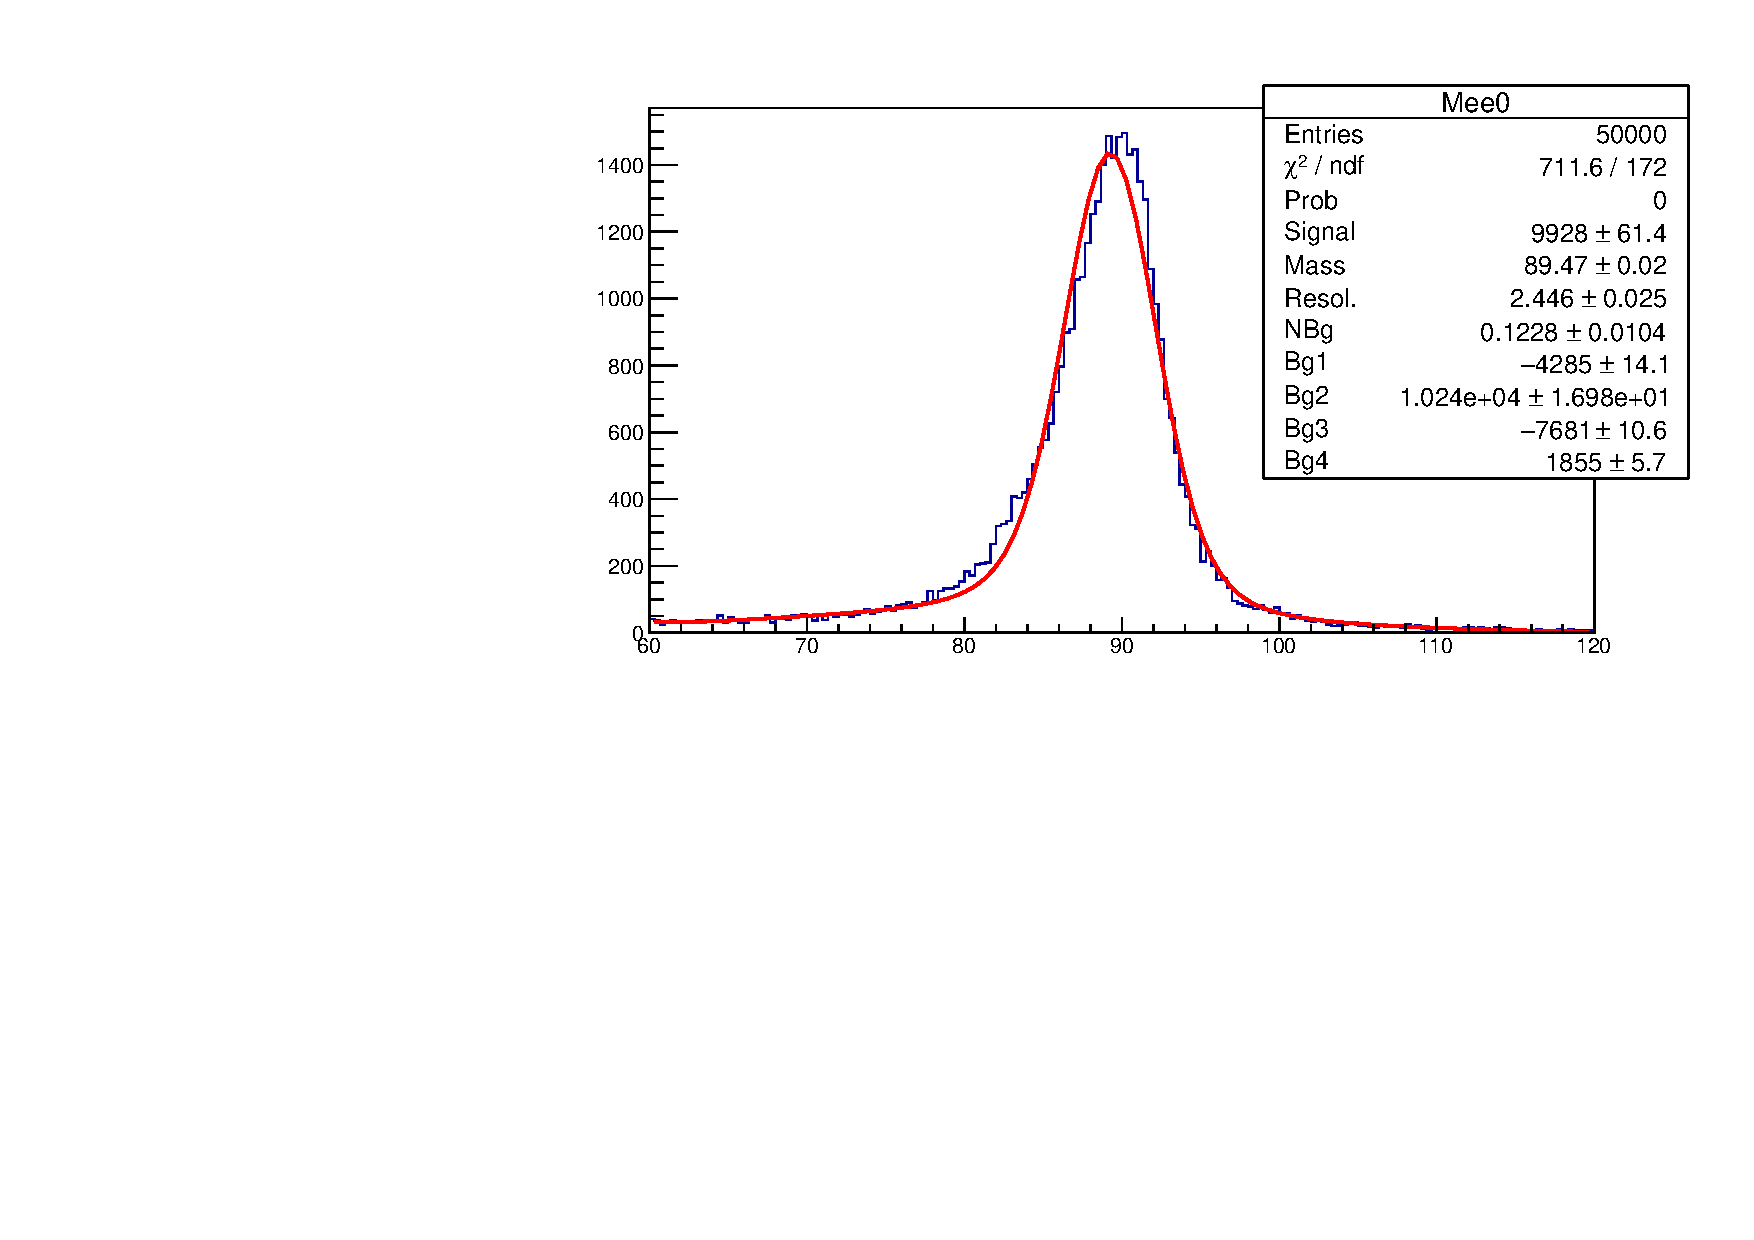
\includegraphics[width=\linewidth]{P1_pics/calibration/Zee_fit_no_calibration.pdf}
		\subcaption{before our calibration}
	\end{subfigure}
\begin{subfigure}{.49\linewidth}
	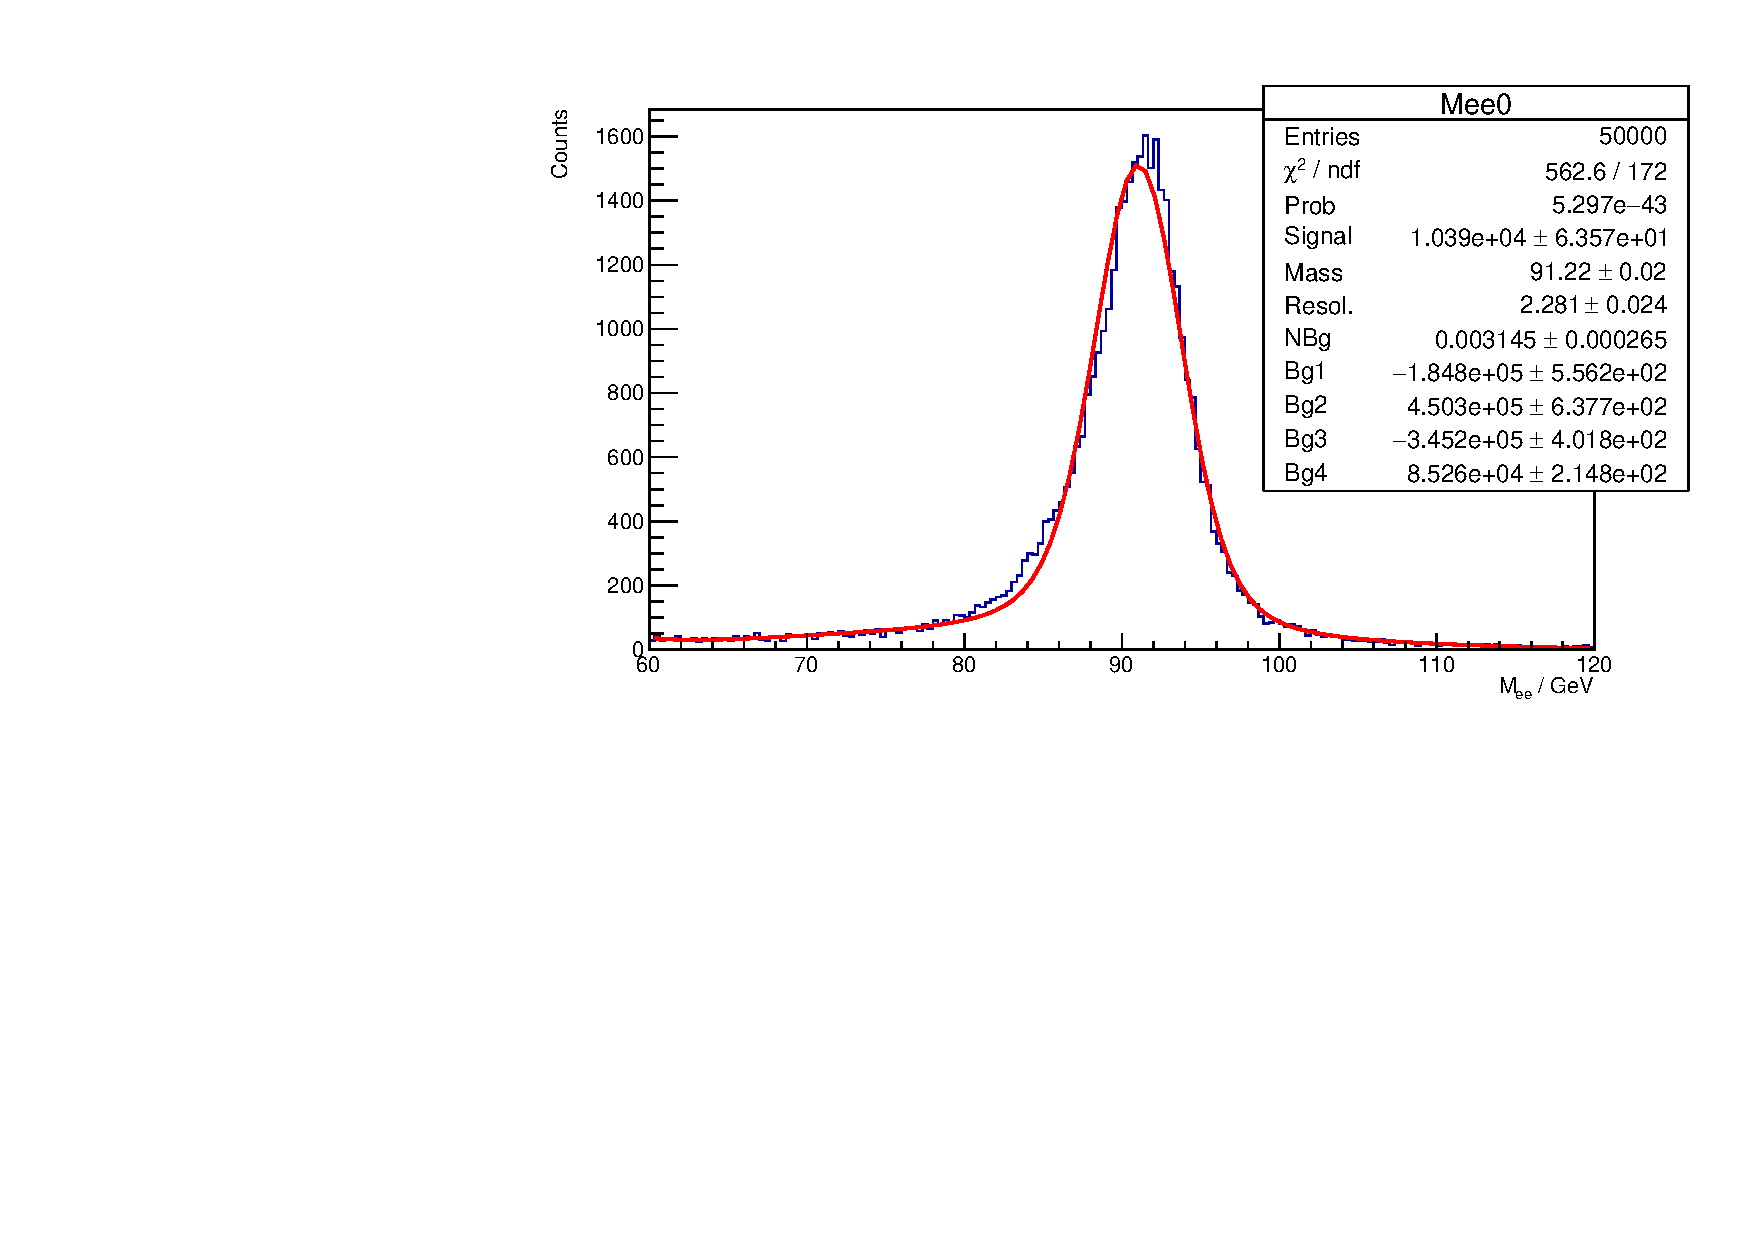
\includegraphics[width=\linewidth]{P1_pics/calibration/Zee_fit_calibration.pdf}
	\subcaption{after our calibration}
\end{subfigure}
\caption{results of fitting the invariant mass peak with and without our calibration}
\label{fig:calib}
\end{figure} 

\subsection{Part 3: Measurement of the W-Boson Mass}
After the initial calibration of the electrons we now will measure the W-Boson mass. For this measurement we take a look at simulated datasets with differing W-Boson masses  to create a gauge curve and a real ATLAS dataset. The data was taken in the $W\to e\nu$ channel. Since the energy of the $\nu$ can't be captured easily, we will use the  transverse momentum distribution to determine the position of the \textsc{Jacobi} peaks. Finally we will investigate the systematic errors and discuss them.

\noindent In table \ref{tab:datasets} the used datasets and their properties are listed.
\begin{table}[htbp]
	\centering
	\begin{tabular}{|c|c|c|}
		\hline
		dataset& dataset abbreviation & description  \\
		\hline
		$W\to e\nu$ & Wenu & ATLAS data with $W\to e\nu$  candidates \\
		$Z\to ee$ & Zee & ATLAS data with $Z\to ee$  candidates \\
		simulated $W\to e\nu$ & MCW75 & MCW75 $W\to e\nu$  simulated signal data, $m_W=75$GeV \\
		simulated $W\to e\nu$ & MCW78 & MCW78 $W\to e\nu$  simulated signal data, $m_W=75$GeV \\
		simulated $W\to e\nu$ & MCW79 & MCW79 $W\to e\nu$  simulated signal data, $m_W=75$GeV \\
		simulated $W\to e\nu$ & MCW80 & MCW80 $W\to e\nu$  simulated signal data, $m_W=75$GeV \\
		simulated $W\to e\nu$ & MCW81 & MCW81 $W\to e\nu$  simulated signal data, $m_W=75$GeV \\
		simulated $W\to e\nu$ & MCW82 & MCW82 $W\to e\nu$  simulated signal data, $m_W=75$GeV \\
		simulated $W\to e\nu$ & MCW83 & MCW85 $W\to e\nu$  simulated signal data, $m_W=75$GeV \\
		QCD background & QCD & background extracted from ATLAS data\\
		\hline
	\end{tabular} 
	\caption{Used datasets. Taken from \cite{manual}.}\label{tab:datasets}
\end{table}

\subsubsection{Pre lab questions II}
We will answer here the mandatory pre lab questions given in the manual for the main part \cite{manual}.
\subsubsection*{Question A}
\emph{As before, the analysis is based on ROOT trees. One of the tree variables is \texttt{ptw} - the estimated transverse momentum of the W boson candidate. This variable can be constructed from the other tree variables. Please think about how this could be done. The tree variables are listed in section B.}

The transverse momentum of the boson follows directly from its decay products. Let $p_{i}, i\in \{e,\nu,W\}$ denote the 4-momentum then we have $$p_W=p_e+p_\nu.$$ Obviously this holds also for the two transversal components.
\subsubsection*{Question B}
\emph{When fitting measurements to a linear function, the two parameters of a best fit straight line are $y$-intercept and slope. The errors on these parameters are typically correlated. Using these parameters for the error analysis will require a treatment that takes correlations into account. For example the simplest form of Gauss’ error propagation law requires that the errors are uncorrelated. Please look up the correct form of the Gauss error propagation law in the presence of correlations. You will need that for the final error on the $W$ mass.}

The error propagation law for two correlated errors $\sigma_a,\sigma_b$ for a function $f(a,b)$ is given as \cite{errors}

\begin{equation}
\sigma_f^2=\left(\frac{\partial f}{\partial a}\cdot \sigma_a\right)^2+\left(\frac{\partial f}{\partial b}\cdot \sigma_b\right)^2+2\frac{\partial f}{\partial a}\frac{\partial f}{\partial b}\cdot\sigma_{ab}
\label{eq:err}
\end{equation}


\subsubsection{Verification of the electron calibration}
Since we used the $Z\to ee$ decay to calibrate the detector and also the $Z$ mass $m_Z$ is well known, we will use it to verify our calibration. We applied different cuts on the datasets to verify the stability of our calibration. In figure \ref{fig:calibration_verification} the ATLAS-data (blue), simulated background (yellow) and $Z\to ee$-decays (green) are depicted. 

We looked at three different cut selections. The first cut filters all events that include jets (hadrons). Since our observed $Z$ decay contains only lepton-products this cut is intuitive. The second cut filters all events of high energy neutrinos. Because this energy isn't measured directly, we filtered the missing energy $\not$$E_t<30$GeV. Last we applied both cuts simultaneously. 
\begin{figure}[h]
	\centering
	\begin{subfigure}{.49\textwidth}
		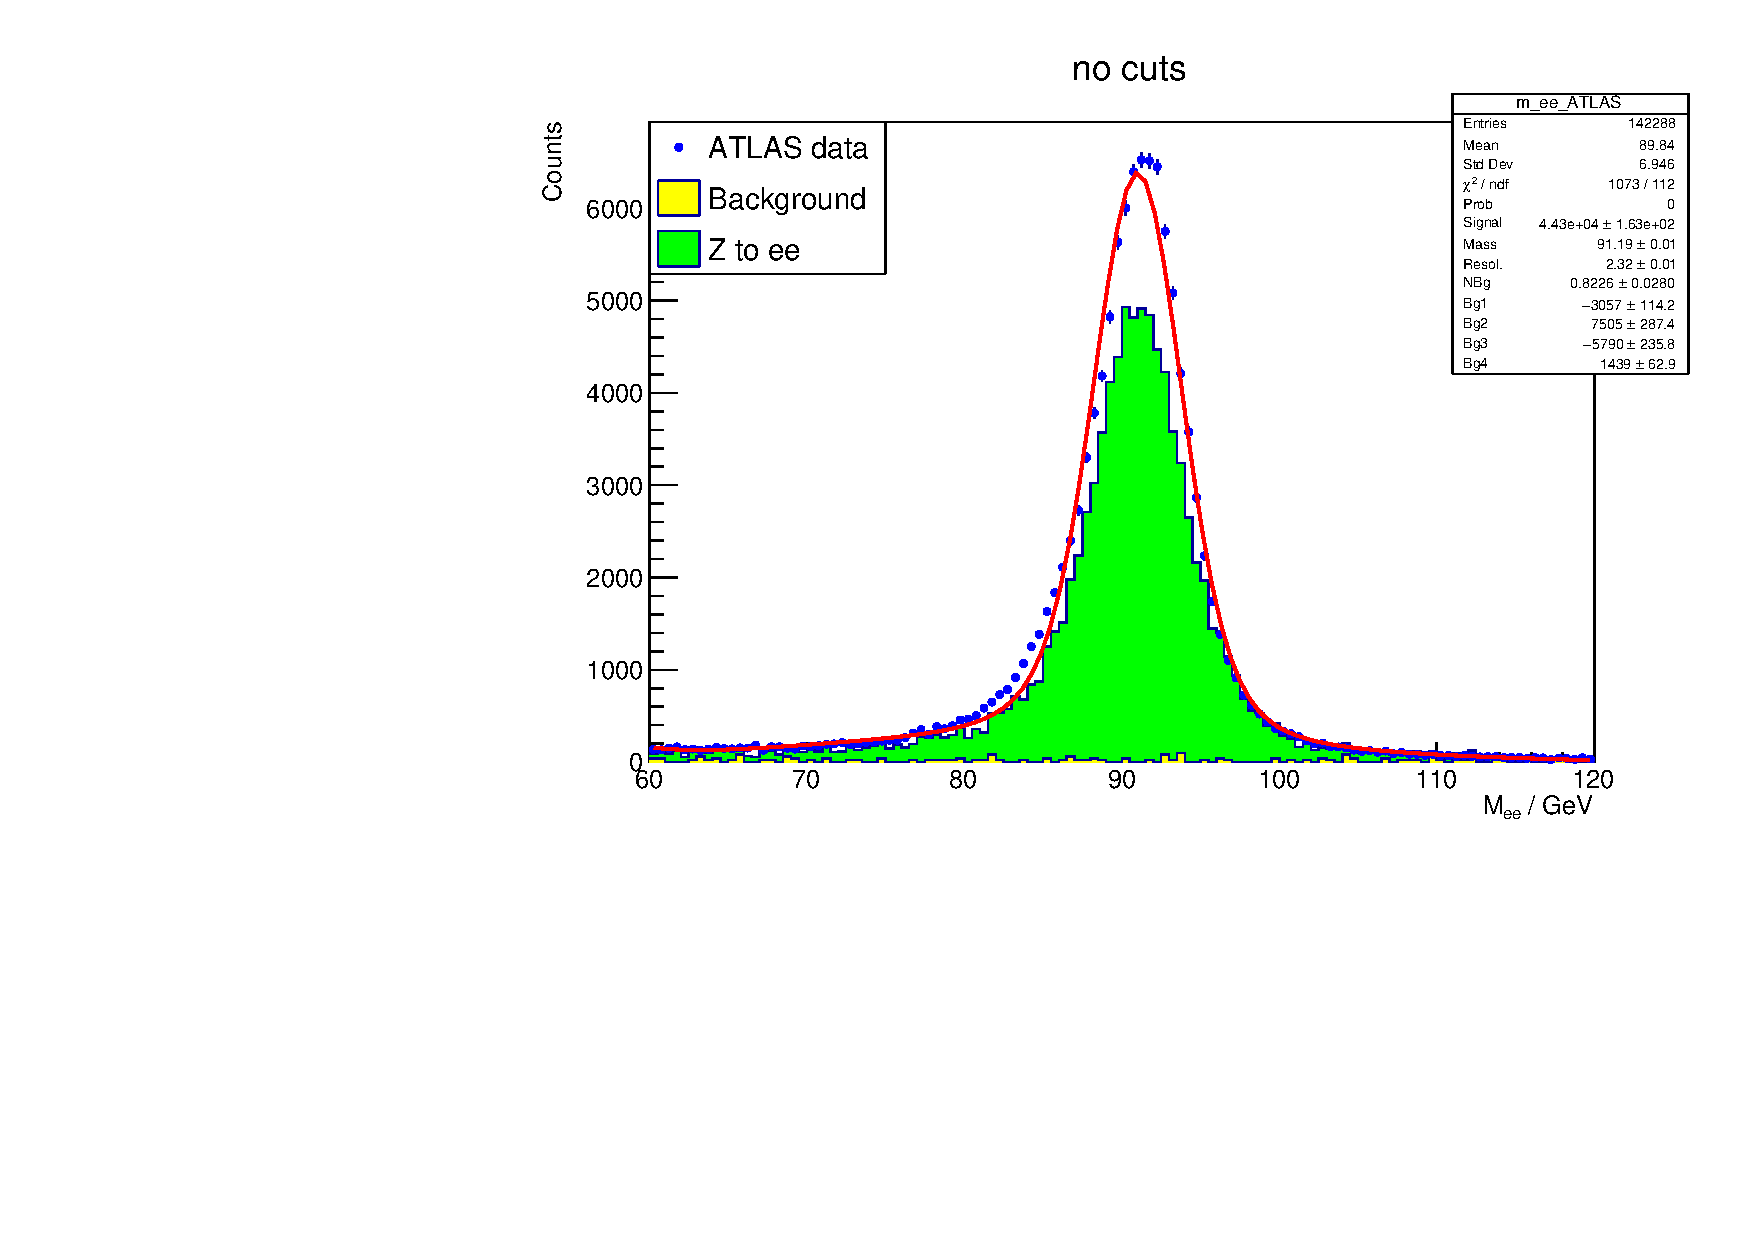
\includegraphics[width=\linewidth]{P1_pics/calibration/zee_fit_no_cut.pdf}
		\caption{}
	\end{subfigure}
%	\begin{subfigure}{.49\textwidth}
%		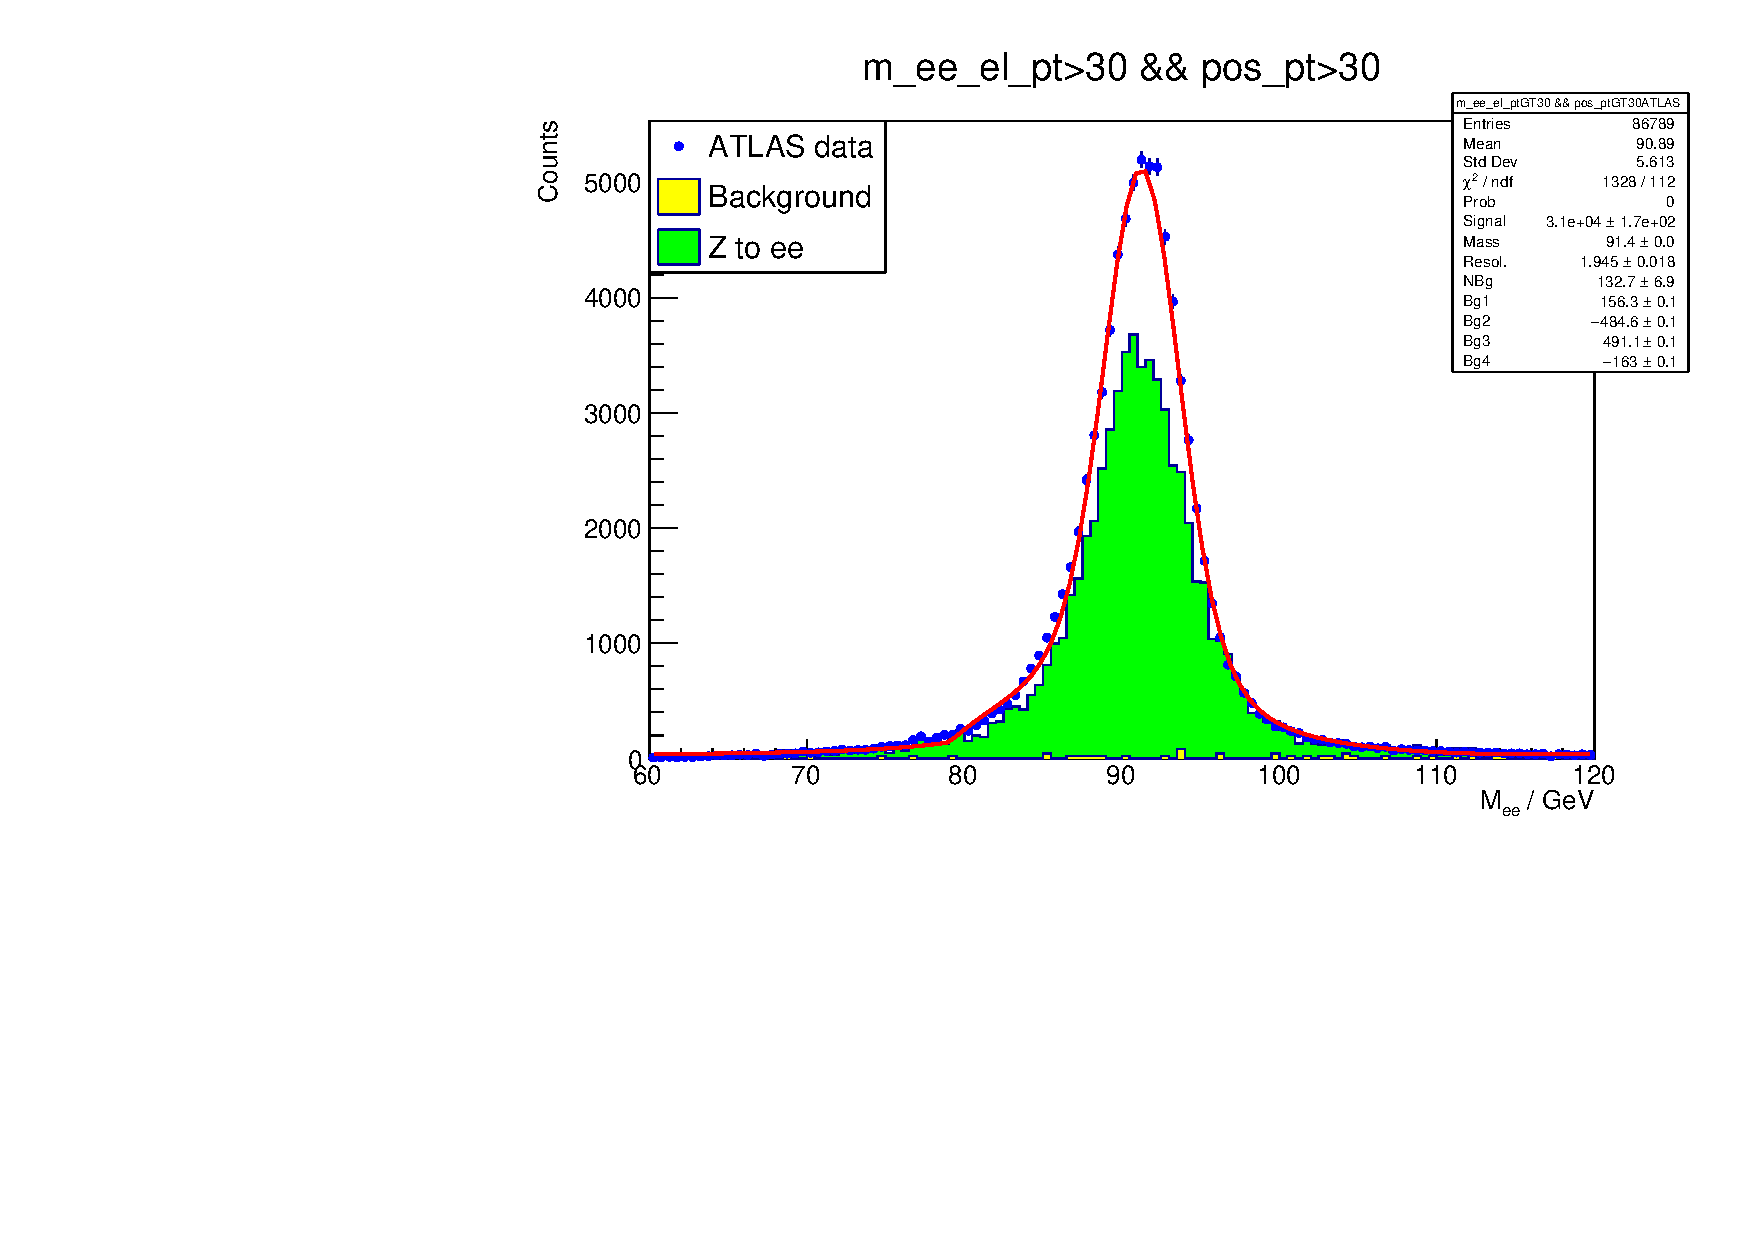
\includegraphics[width=\linewidth]{P1_pics/calibration/zee_fit_high_pt.pdf}
%		\caption{}
%	\end{subfigure}
	\begin{subfigure}{.49\textwidth}
		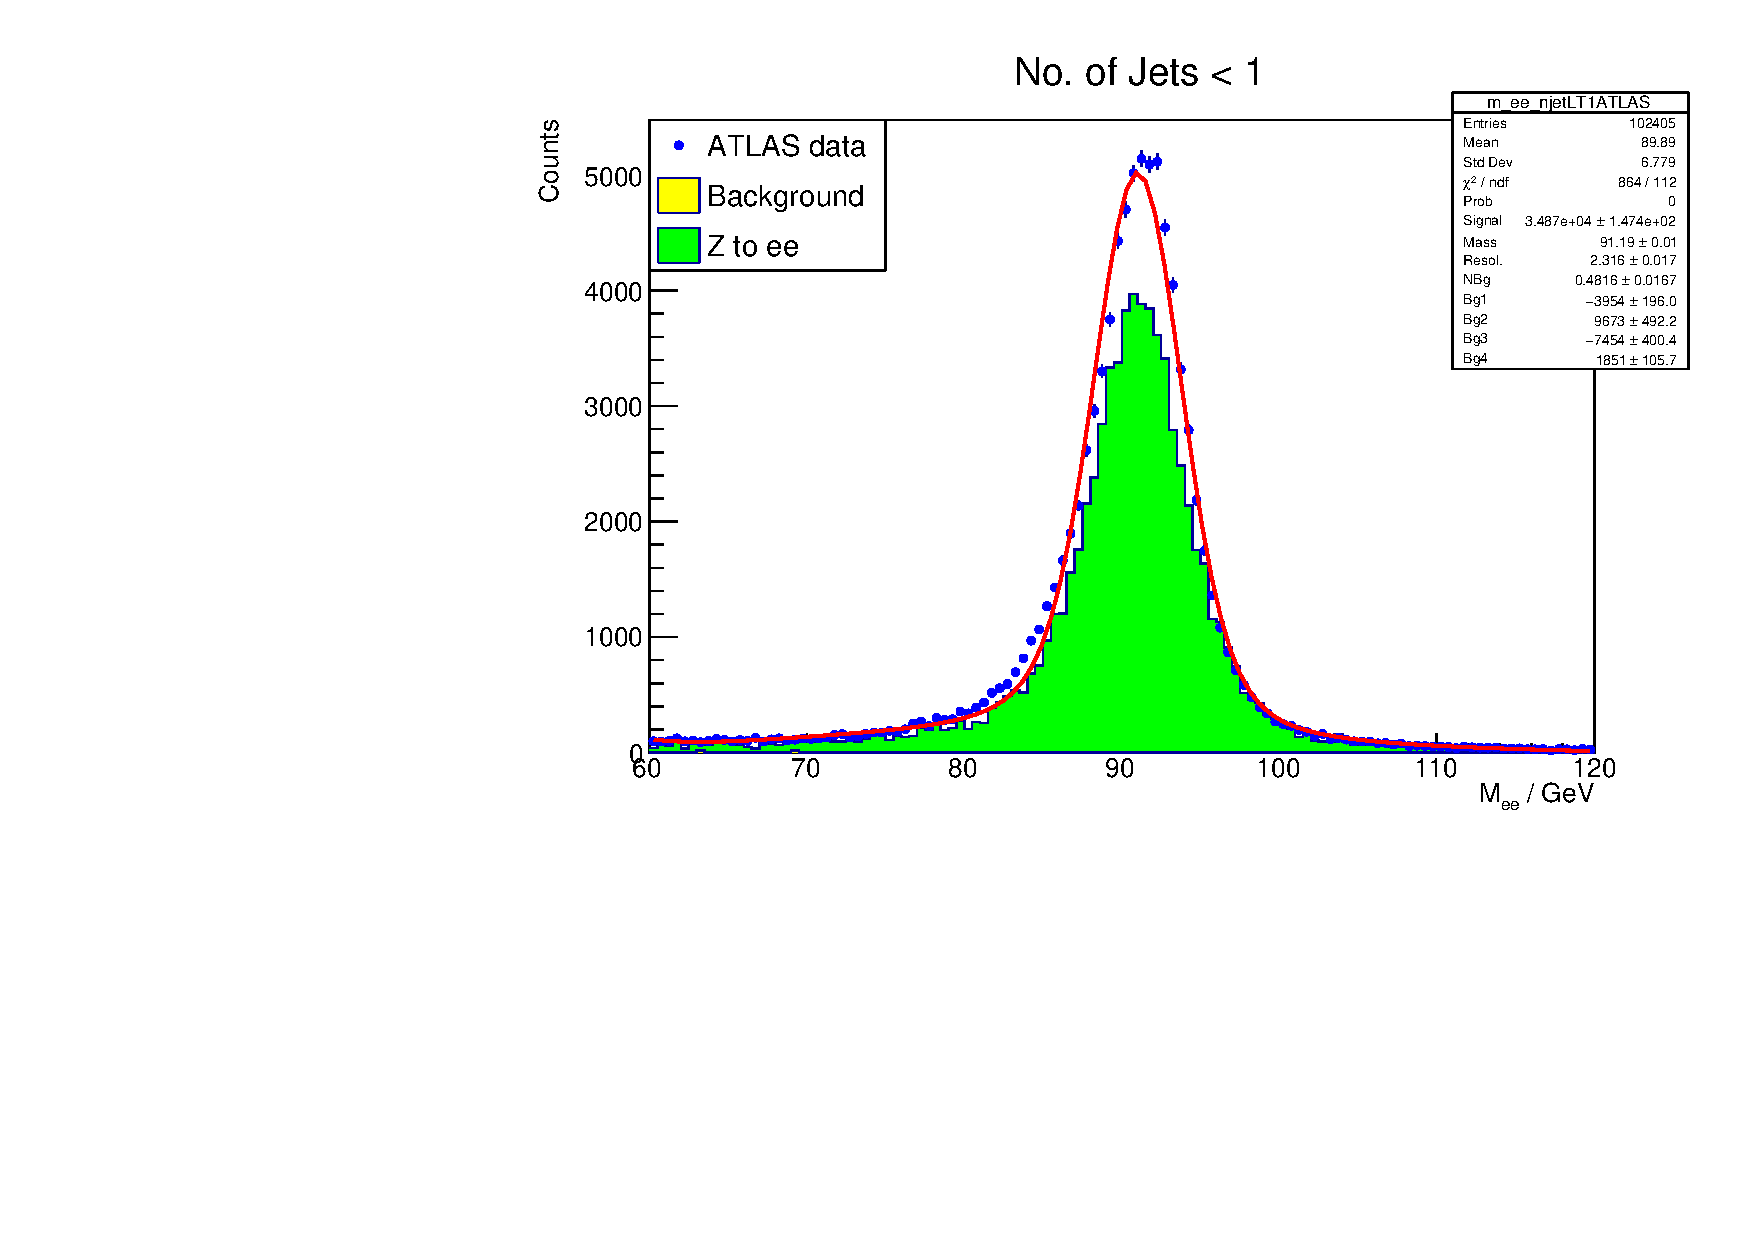
\includegraphics[width=\linewidth]{P1_pics/calibration/zee_fit_njet.pdf}
		\caption{}
	\end{subfigure}
	\begin{subfigure}{.49\textwidth}
		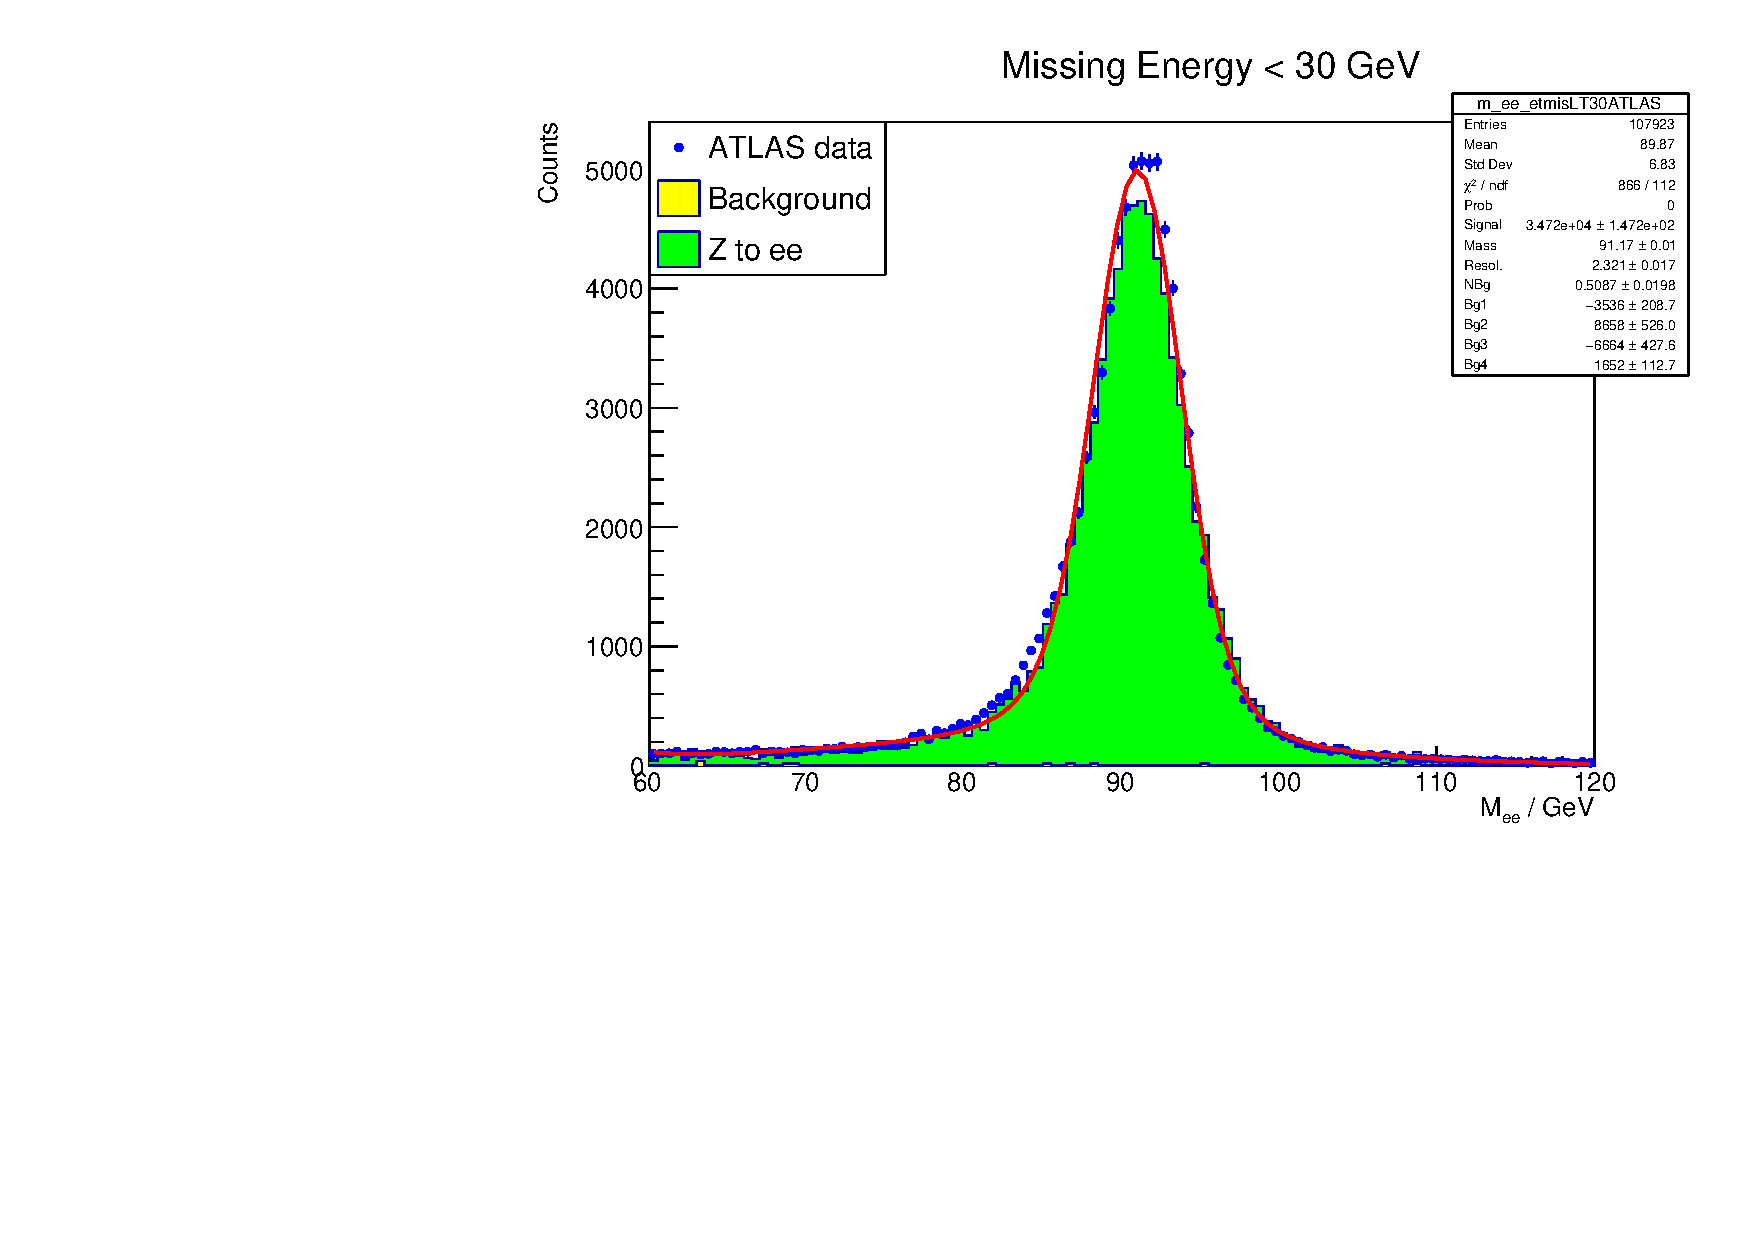
\includegraphics[width=\linewidth]{P1_pics/calibration/zee_fit_miset.pdf}
		\caption{}
	\end{subfigure}
	\begin{subfigure}{.49\textwidth}
		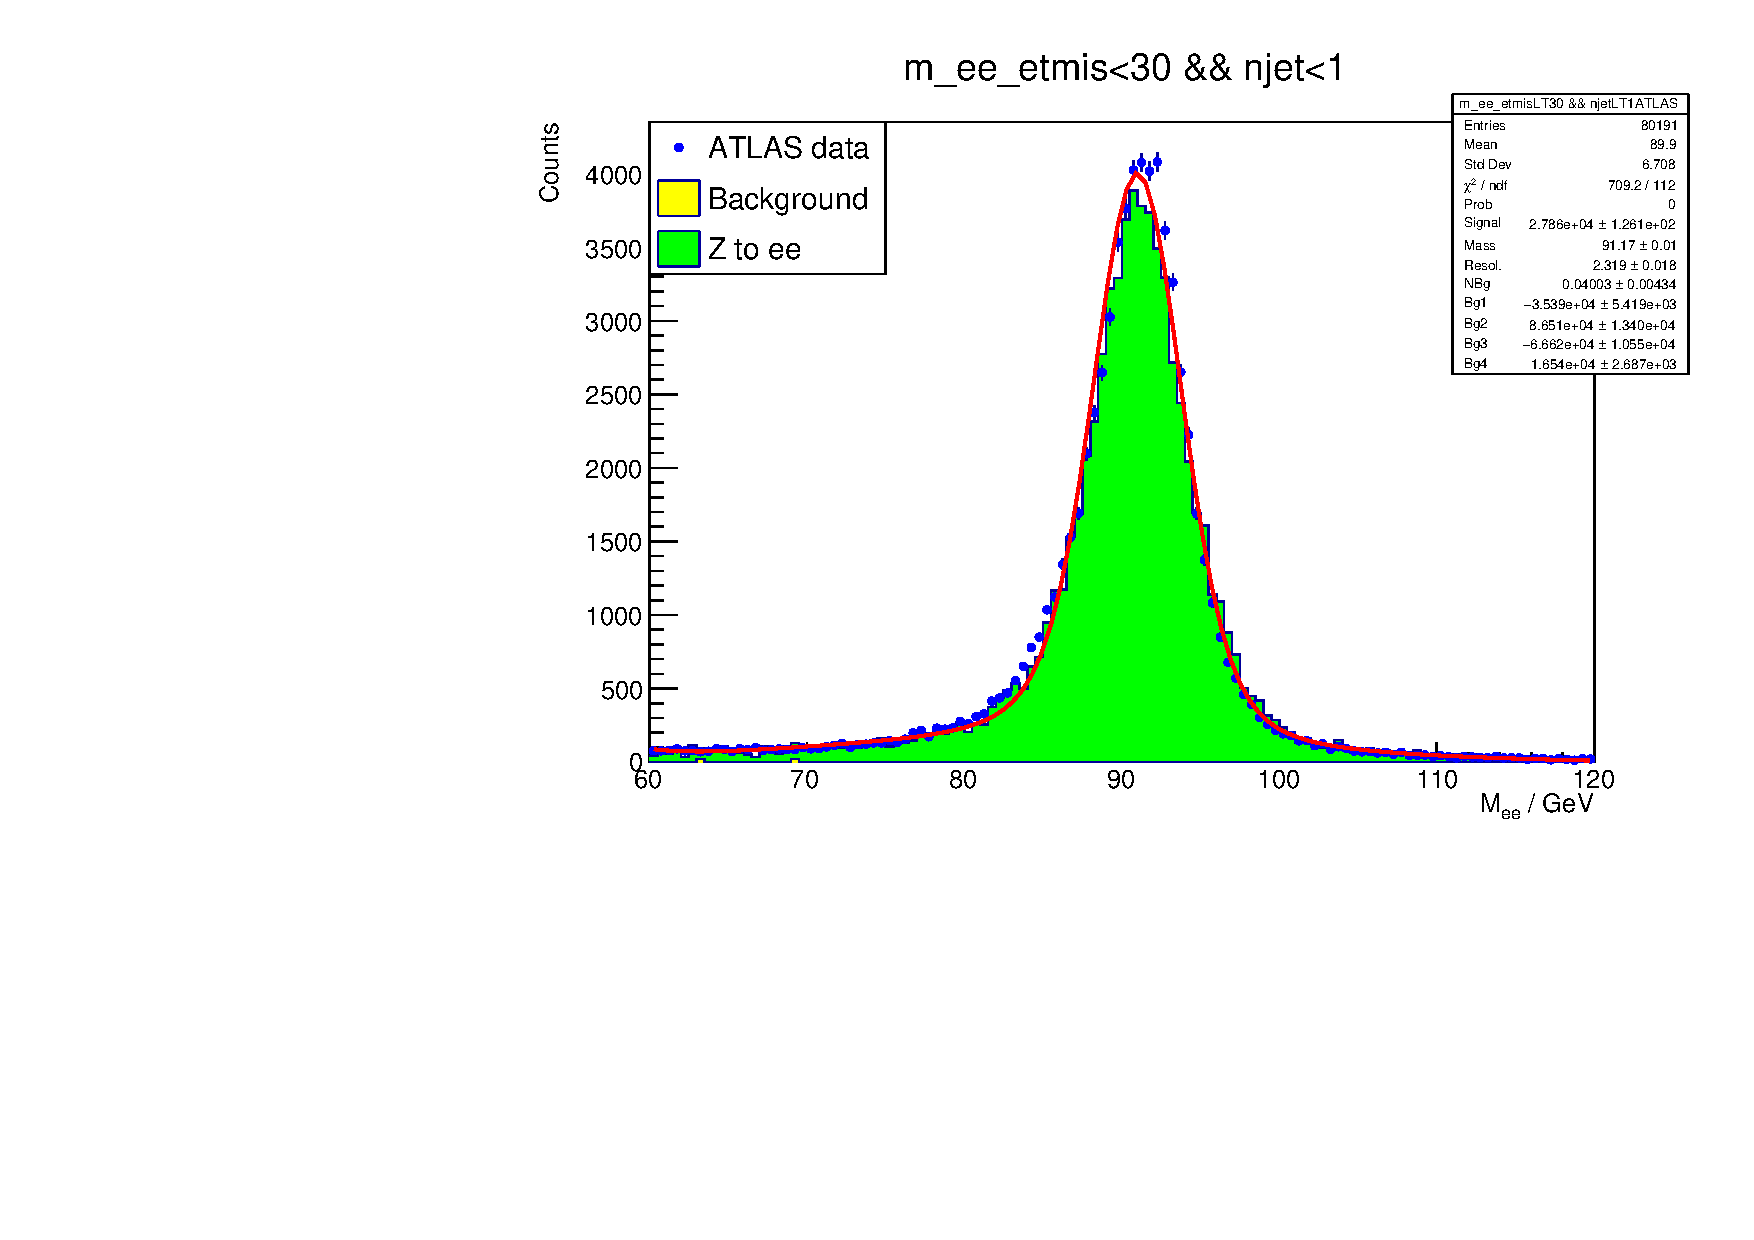
\includegraphics[width=\linewidth]{P1_pics/calibration/zee_fit_miset_njet.pdf}
		\caption{}
	\end{subfigure}
	\caption{Invariant mass spectra of $Z\to ee$ decays with different cuts applied. ATLAS data (blue), simulated $Z\to ee$ decay events (green) and background (yellow)}\label{fig:calibration_verification}
\end{figure}

With none and all applied cuts the literature value of  $m_W=(91.1876\pm 0.0021)$ GeV \cite{pdg} lies in the error of our results. For both applied cuts, we measured the $Z$-Boson mass $$m_Z=(91.17\pm0.01)\text{ GeV}.$$
This result verifies, that our calibration is good enough to proceed to the next task and does not need any further adjustments.

\subsubsection{Inspection of Kinematic Variables }
The QCD background originating from jets can be extracted from measured ATLAS data. This will provide the correct shape of the background but it will not match the actual data size. It has thus to be properly normalized using a scale factor that matches the data. We can simply set the scale factor that applies to all plots that contain QCD background. It is advisable to look at regions with a lot of background to estimate the scale factor well by eye.

In this section we briefly investigate the influence of jets on the $W$-Boson $p_t$ spectrum and estimate the QCD-factor by eye.

Our first estimation of the QCD factor is $0.30$. In the Appendix \ref{fig:eyeballed_cuts} the first estimate can be found for the properties $p^e_t$ (electron transverse momentum),   $E_t^{\text{iso}}$ (electron isolated cone energy \cite{manual}), $n_{\text{jet}}$ (number of jets), $\not$$E_t$ (missing transverse energy) and $p_t^W$ (transverse momentum of $W$ boson). We set it in a way, that the simulated $W\to e\nu$ stack plot almost matched the real ATLAS data. In the next section we will redo this process with higher accuracy.

To investigate the influence of jets, we cut the $p_t$ spectrum for different numbers $N<[1,2,3,4,5]$ of jets. In figure \ref{fig:jet_influence_on_w_mass} those $p_t$ spectra are shown.
\begin{figure}[h]
	\centering
	\begin{subfigure}{.32\linewidth}
		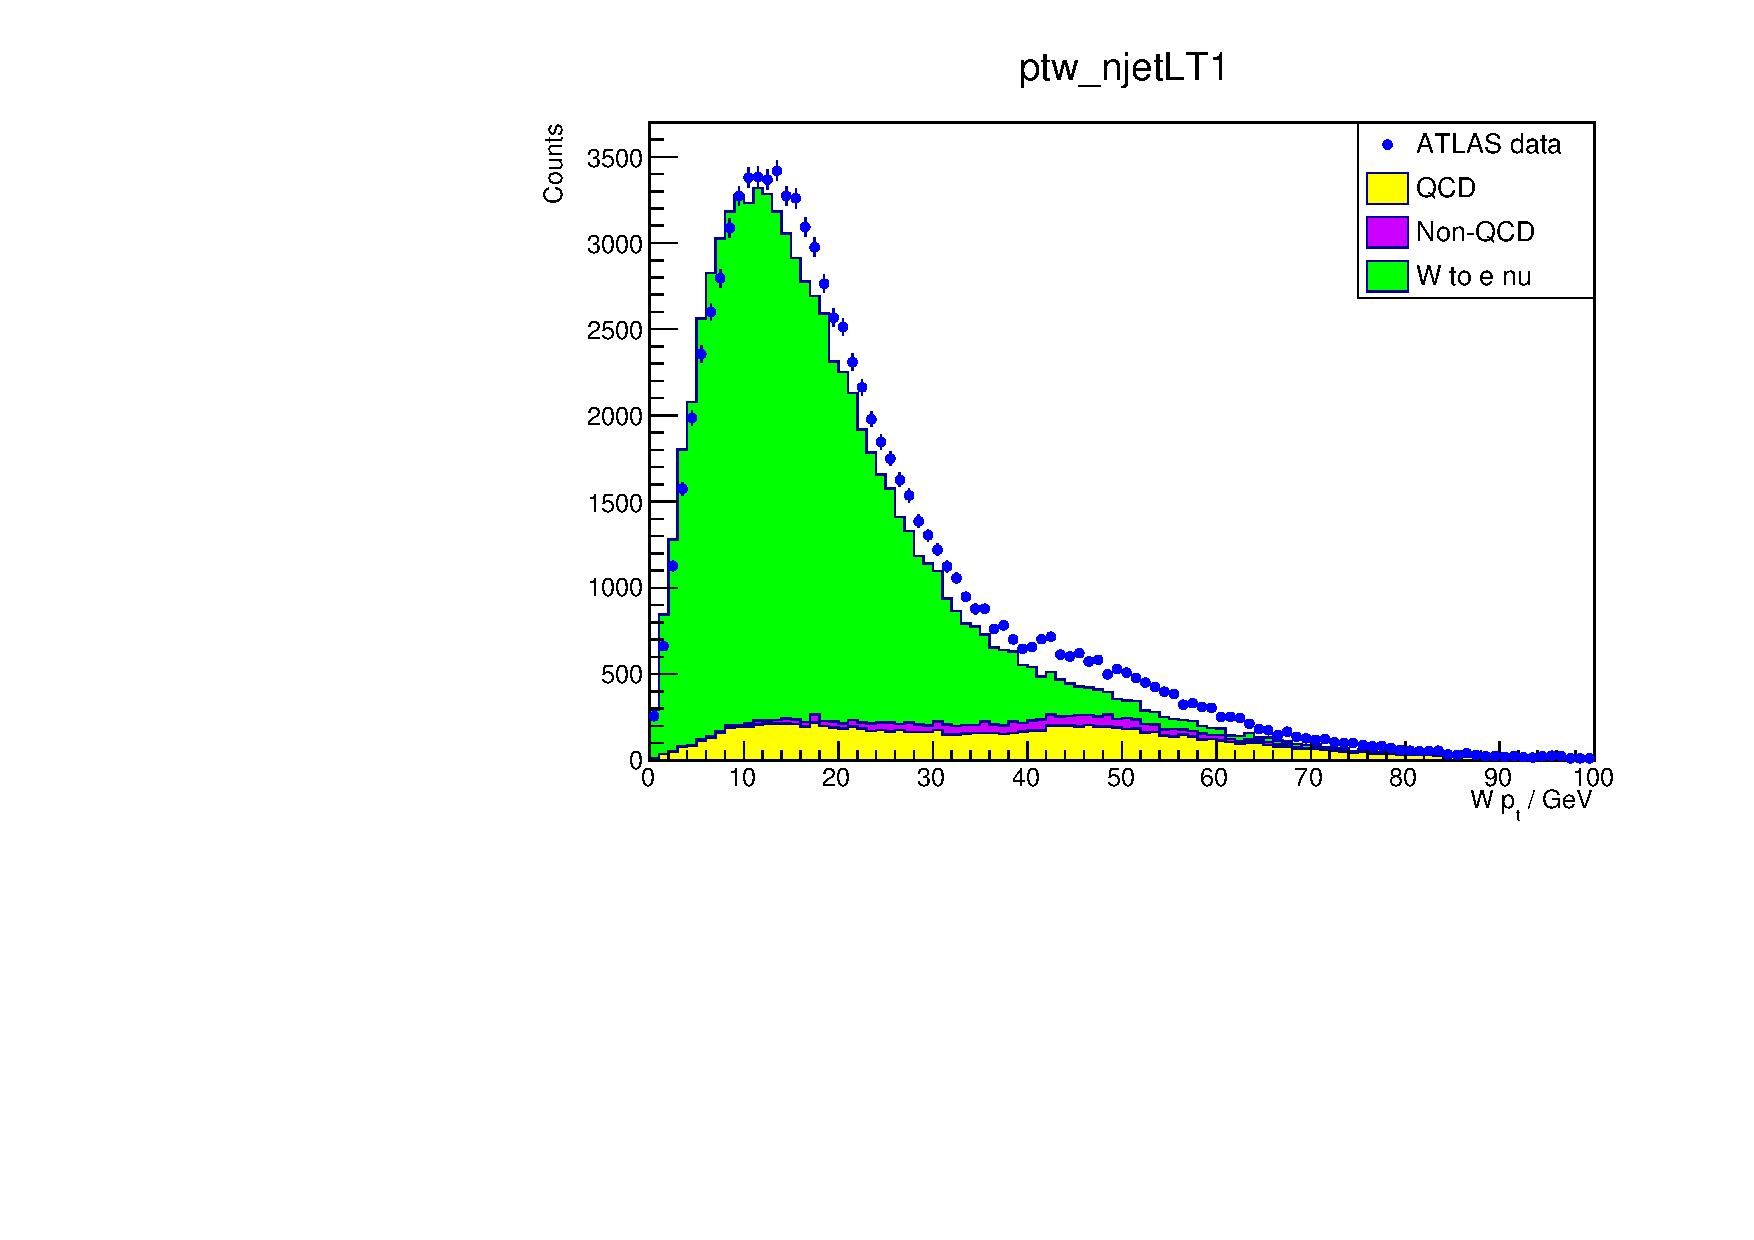
\includegraphics[width=\linewidth]{P1_pics/ptw_jets/ptw_njet0.pdf}
		\caption{}
	\end{subfigure}
	\begin{subfigure}{.32\linewidth}
		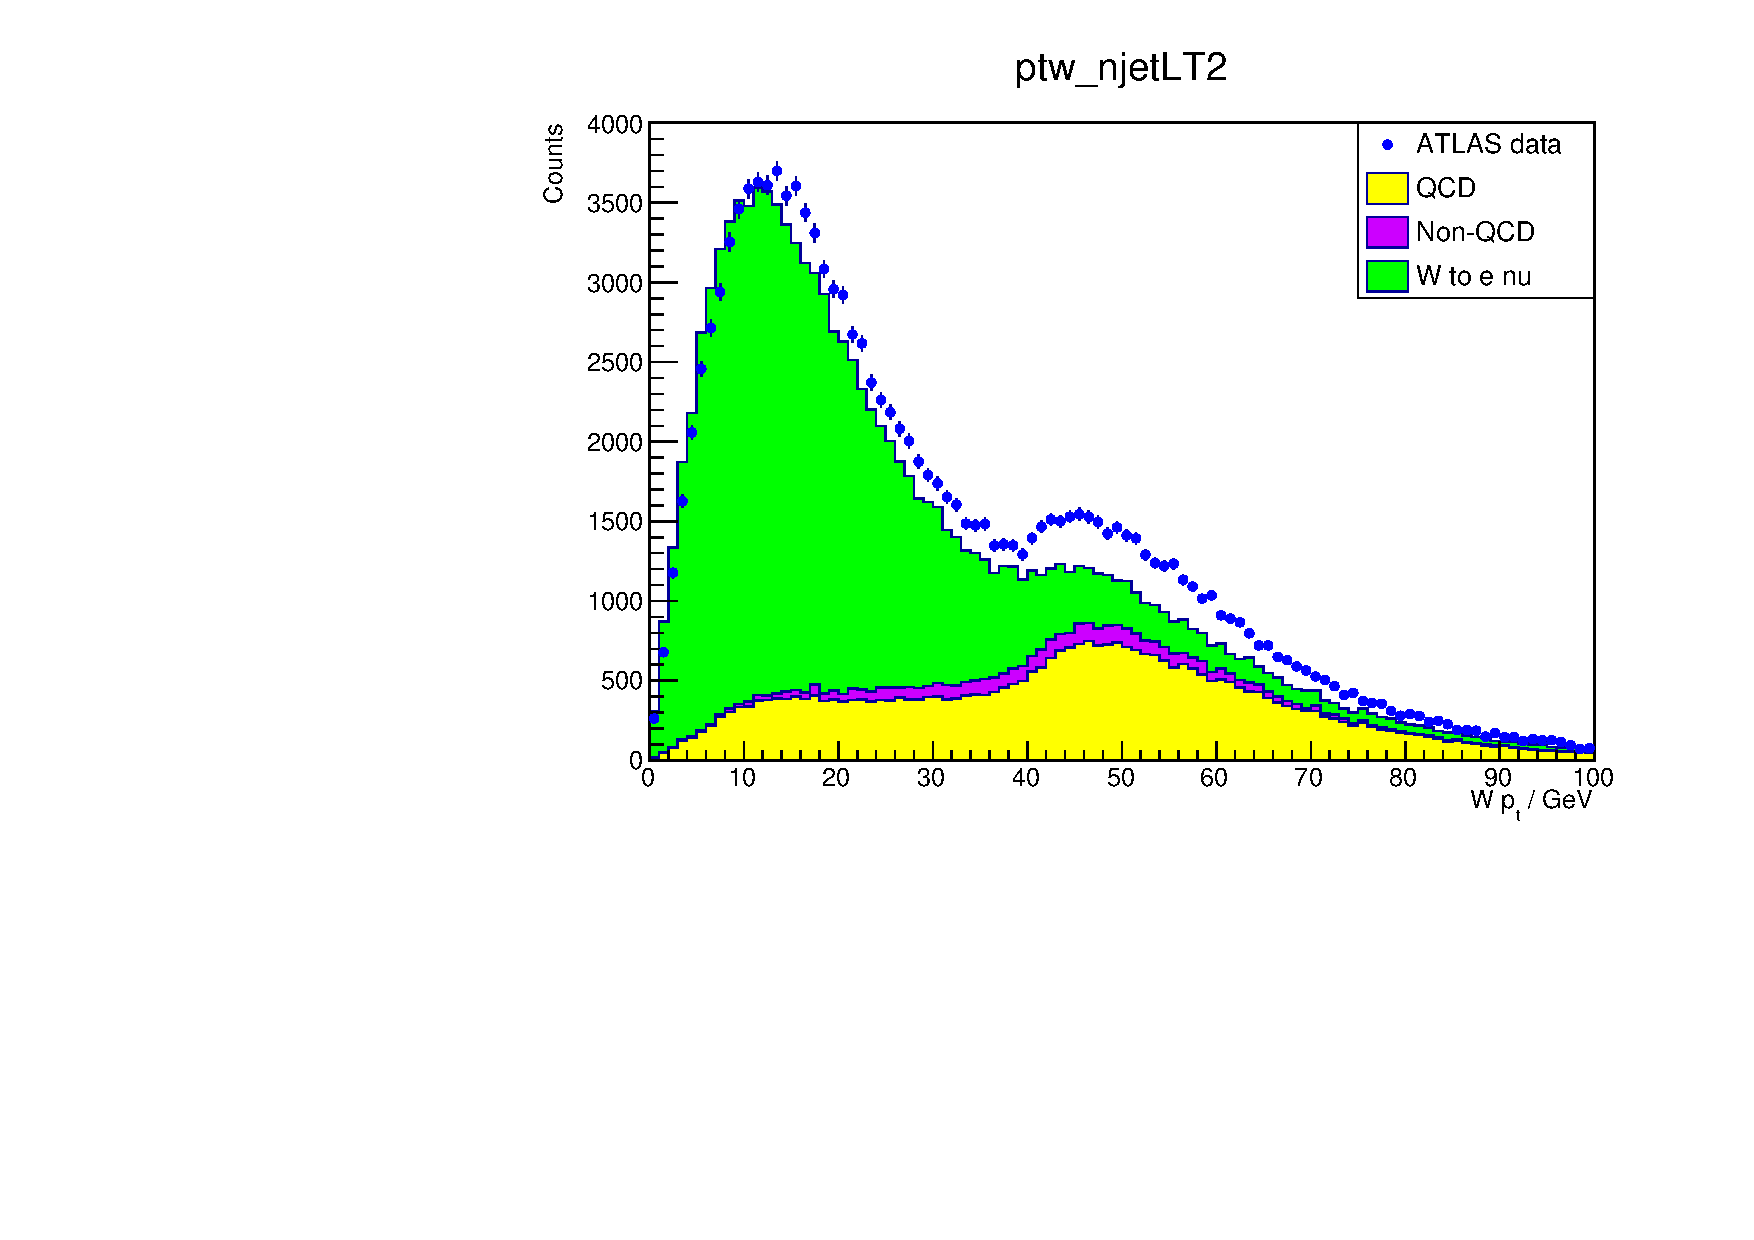
\includegraphics[width=\linewidth]{P1_pics/ptw_jets/ptw_njet1.pdf}
		\caption{}
	\end{subfigure}
	\begin{subfigure}{.32\linewidth}
		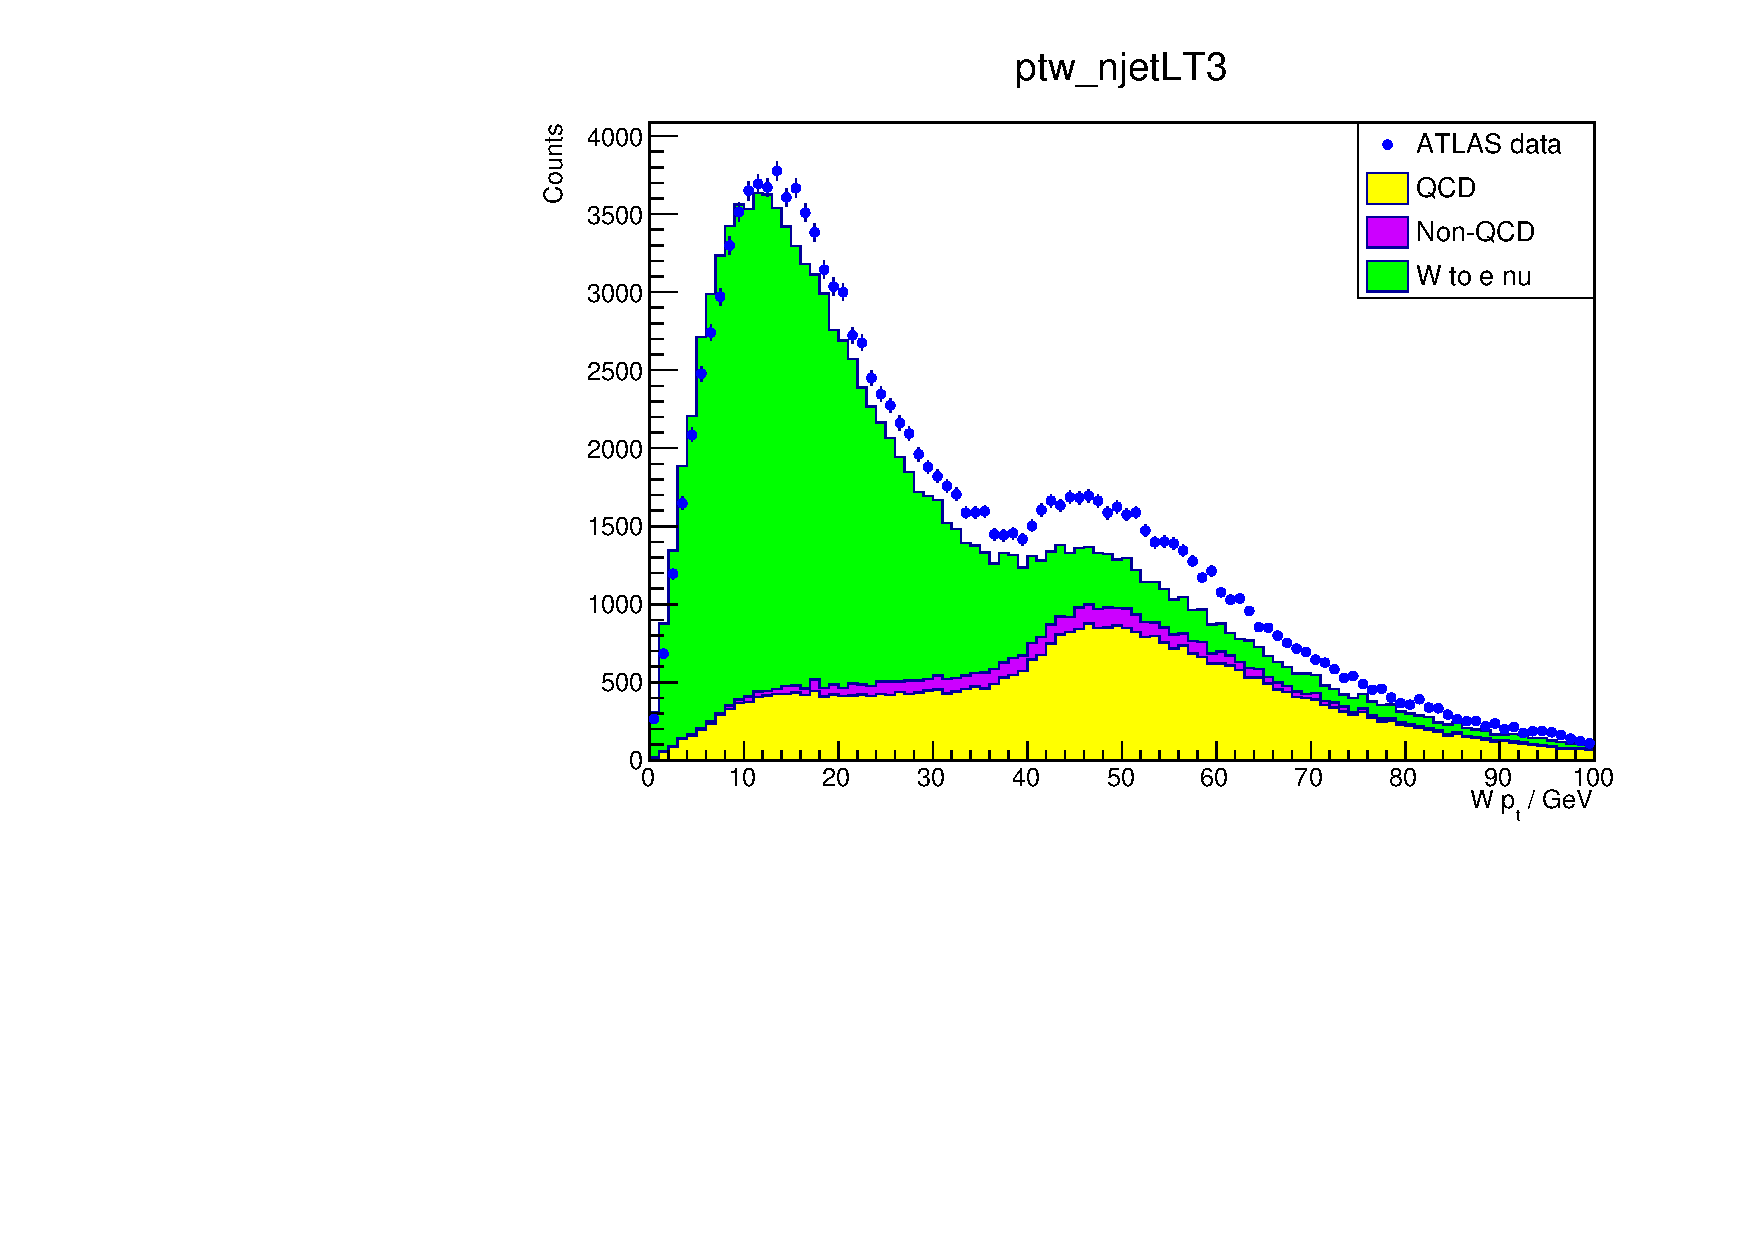
\includegraphics[width=\linewidth]{P1_pics/ptw_jets/ptw_njet2.pdf}
		\caption{}
	\end{subfigure}

	\begin{subfigure}{.33\linewidth}
		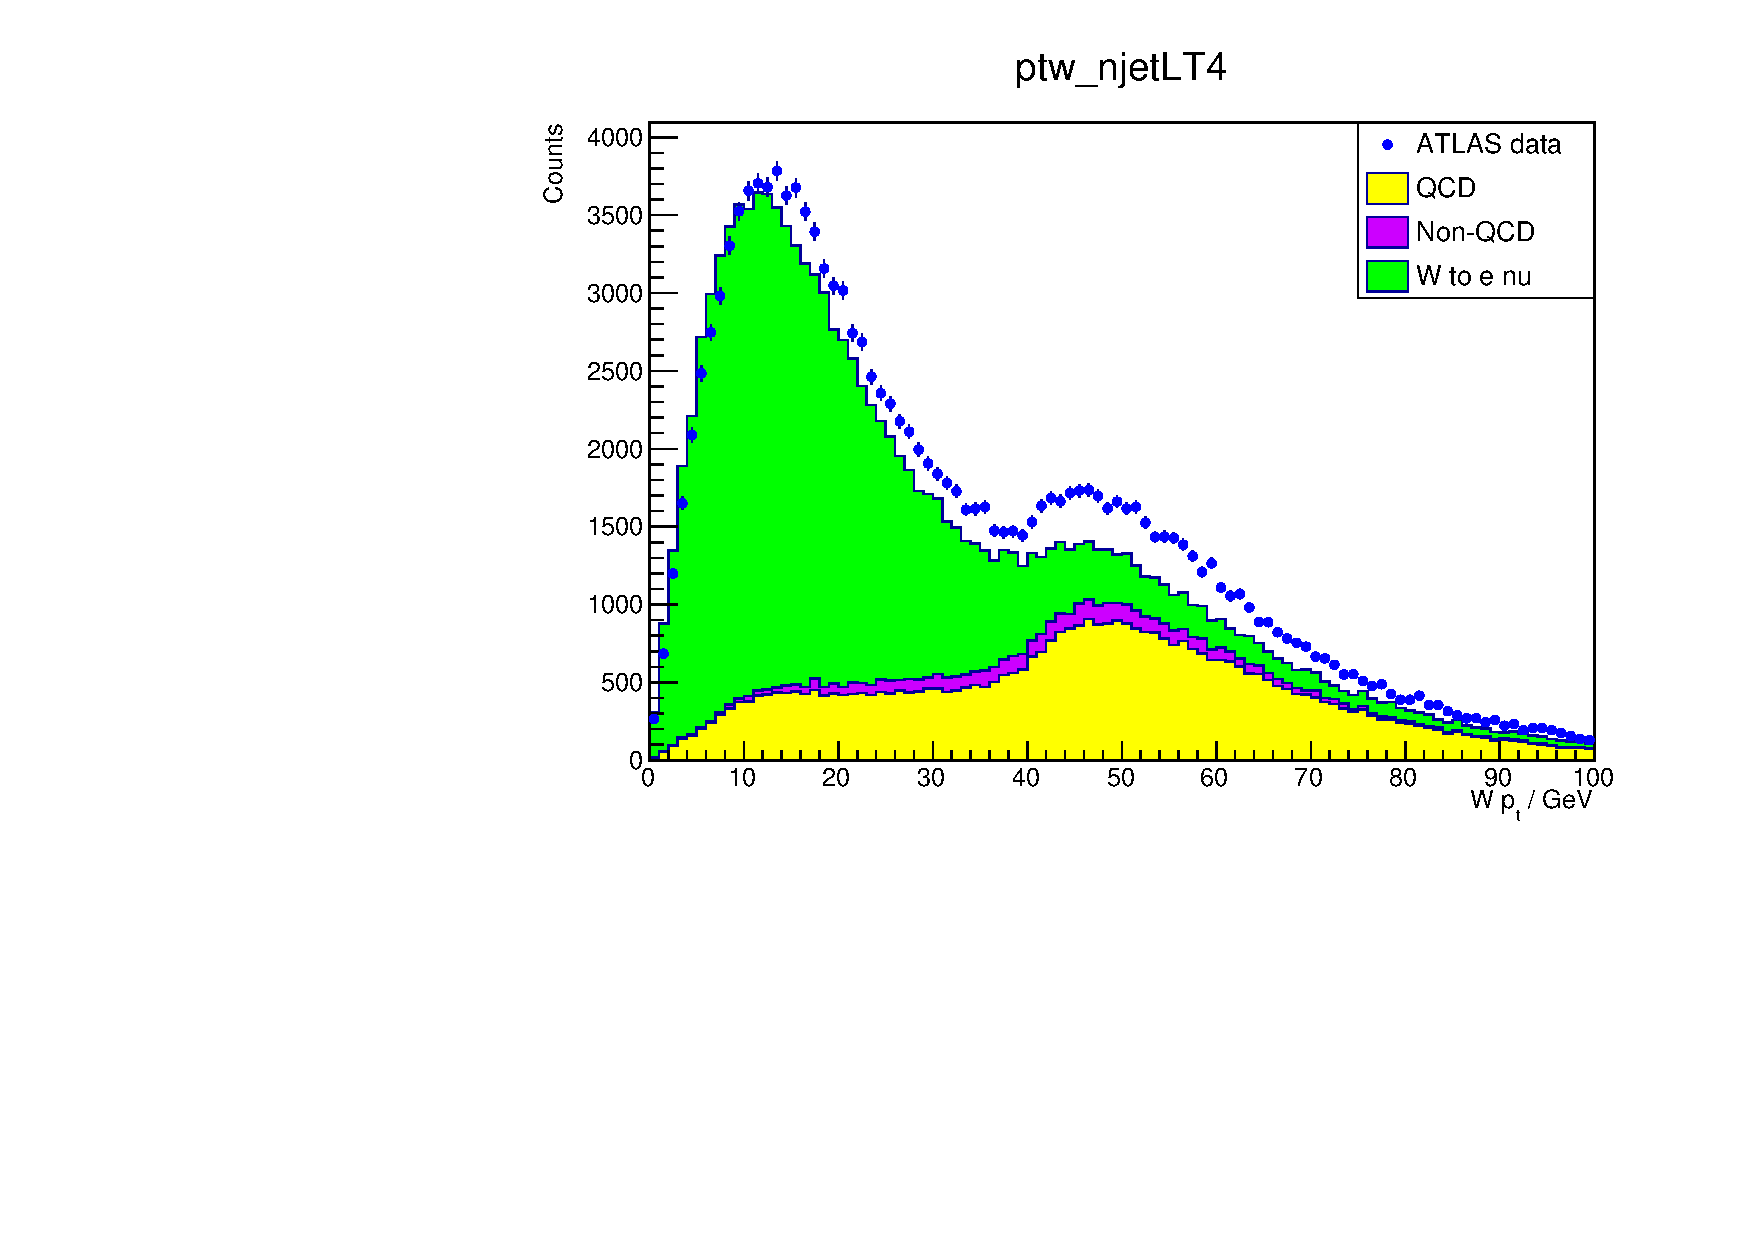
\includegraphics[width=\linewidth]{P1_pics/ptw_jets/ptw_njet3.pdf}
		\caption{}
	\end{subfigure}
	\begin{subfigure}{.33\linewidth}
		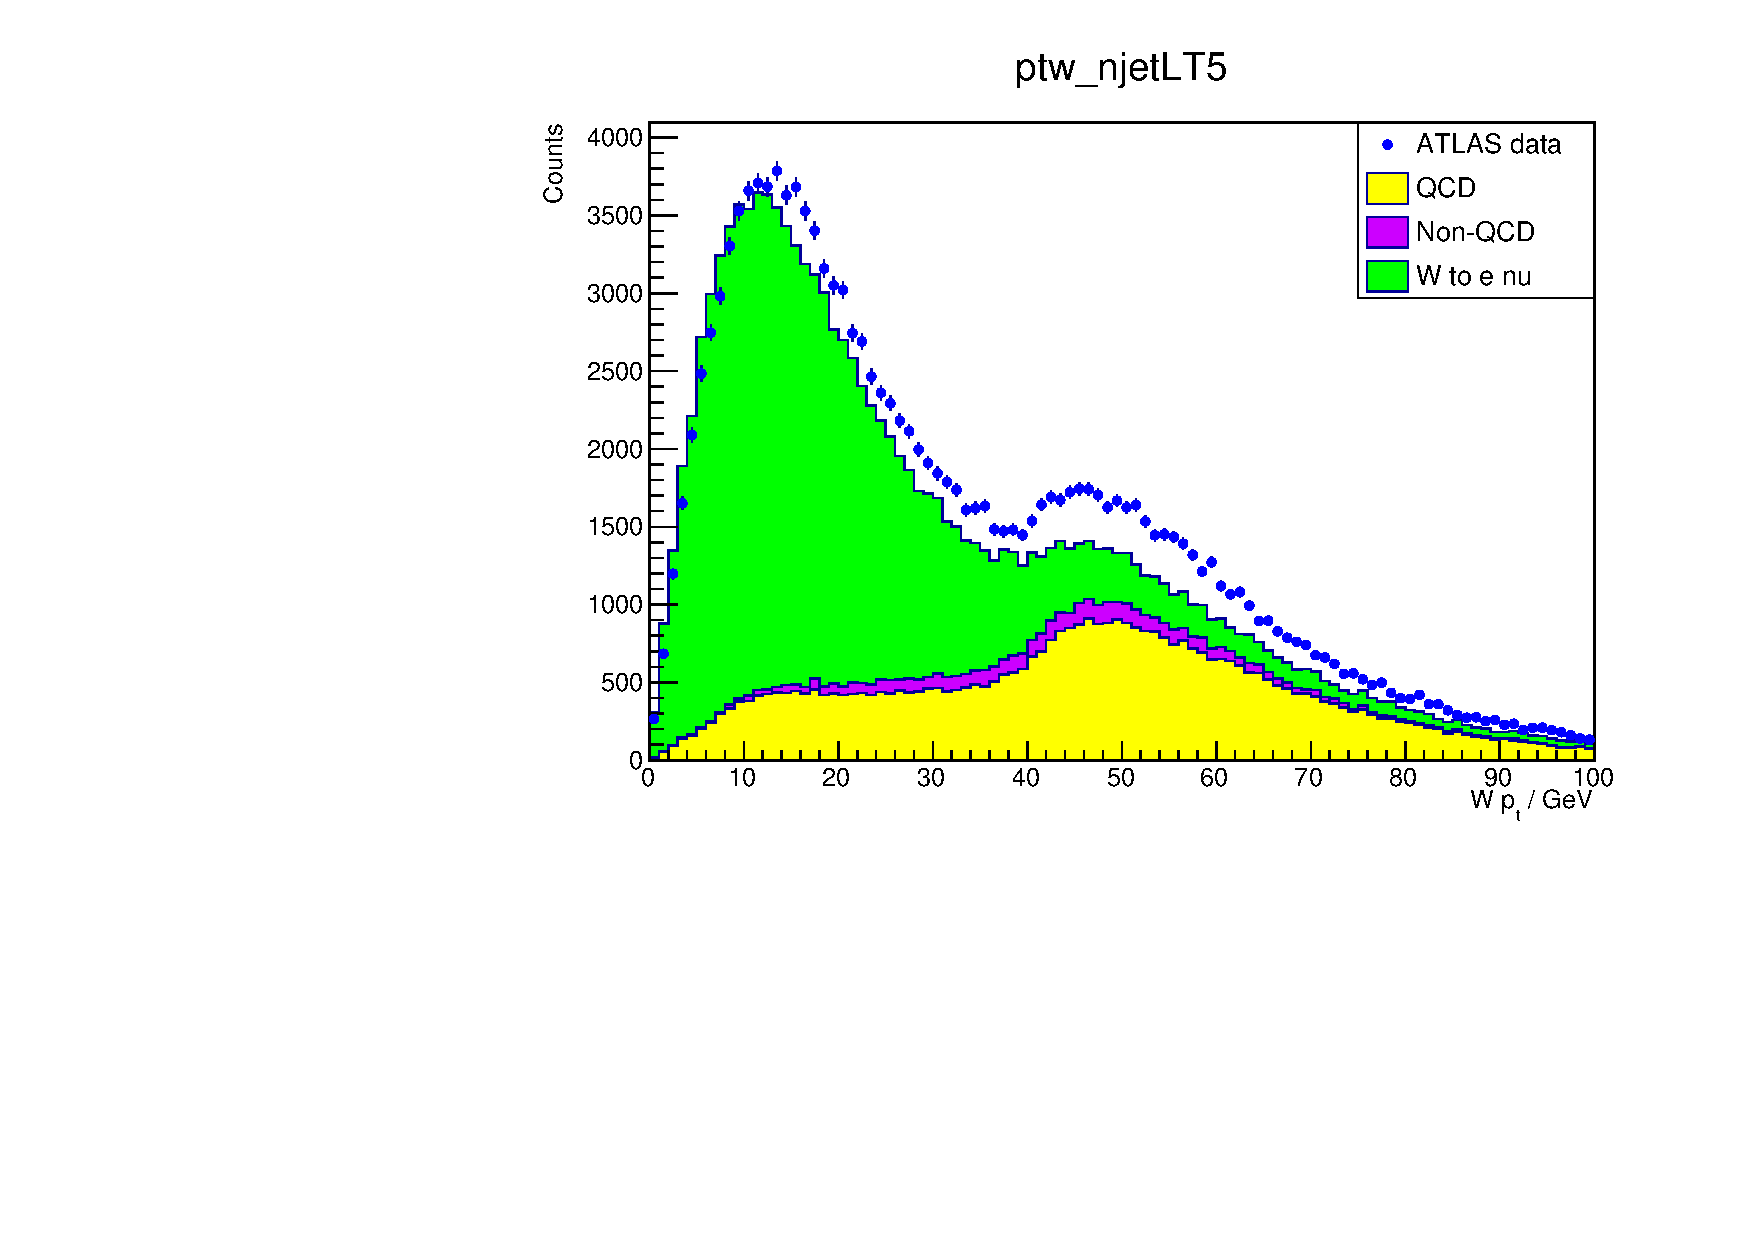
\includegraphics[width=\linewidth]{P1_pics/ptw_jets/ptw_njet4.pdf}
		\caption{}
	\end{subfigure}
	\caption{$W$-Boson $p_t$ spectra for less then 1 to 5 jets (from a $\to$ e)}\label{fig:jet_influence_on_w_mass}
\end{figure}

One can clearly see, that with a rising number of jets the QCD-background grows especially for high transverse momenta of the $W$-boson. But with a rising number of possible jets, the QCD-background grows also slowly. This means, that primarily single jet products have the biggest influence on the QCD-background. The conclusion is, that most likely single jets are produced. This can be explained by additional gluons that have been emitted/absorbed during production (see figure \ref{fig:feyn}) which lead to a higher number of jets and also a non-zero transverse momentum of the bosons.

\subsubsection{Cut selection and the QCD background}\label{sec:cuts}
Since the QCD-background is dominant especially at high energies, we will have to filter it. To do so, we will apply a cut selection and suppress the background. But to do this we must also scale the simulated QCD background such that it matches measured data. 

\begin{enumerate}
	\item \textbf{Cut selection}: We chose our cuts in a way, that the data consists almost of none QCD-background, or in other words, we filtered the parts where QCD-background was dominant. 
	\item \textbf{QCD-scale factor}: To properly filter the QCD-background we applied the simple technique of inverse cut selection. For this we applied the inverse cuts from table \ref{tab:cuts} and set the QCD-scale factor for each property individually so that it matches the ATLAS data. In figure \ref{fig:QCD} is the inverse cut selection shown.
	
	
	Table \ref{tab:cuts} lists our selected cuts with uncertainties (upper and lower limits) and QCD-scale factors. The upper and lower limits will be crucial for the systematic error analysis. Some properties don't have upper and lower limits because in a physical and practical way they would not make any sense.
	\begin{table}[H]
		\centering
		\begin{tabular}{|c|c|c|}
			\hline
			Property & cut & QCD-Scale factor\\
			\hline
			$p^e_t$& >$30^{+2}_{-2}$GeV  & 0.38\\
			$E_t^{\text{iso}}$&$<5^{+2}$GeV& 0.38\\
			$n_{\text{jet}}$&$<1$&0.31\\\
			$\not$$E_t$&$>30^{+2}_{-2}$GeV&0.33\\
			$p_t^W$&$<40^{+2}_{-2}$GeV&0.33\\
			\hline
		\end{tabular}
		\caption{Cut and QCD-factor selection}\label{tab:cuts}
	\end{table}
	For the QCD-factor follows the mean and the standard deviation
	$$\text{QCD-Scale factor}=0.35\pm0.03$$
	which will be used from now on.
\end{enumerate}
\subsubsection{Initial fits of the electron $p_t$ spectrum}
We want to estimate the \textsc{Jacobi} peak in the transverse momentum spectrum to determine the mass of the $W$ boson. Since the spectrum is smeared from effects discussed in section \ref{sec:theo} what we actually observe is a convolution of a \textsc{Gaussian} with the actual spectrum featuring a sharp \textsc{Jacobi} peak. As a result the actual peak is shifted (symmetrically) towards smaller values. For this reason the point where half as much entries with respect to the peak are observed is estimated as the \emph{actual} \textsc{Jacobi} edge. \cite{manual}

Before creating the gauge curve and deriving the $W$-boson mass, a proper fit interval for the \textsc{Jacobi} peak should be chosen. We did this by varying the the fit range $[x_{\text{min}},x_{\text{max}}]$, checking the value of $\chi^2$ and by evaluating the visual matching of the data and the fit. We found the boundaries
$$x_\text{min}=30_{-5}^0\text{GeV} \text{\phantom{ nuun } and \phantom{ nuun }} x_{\text{max}}=50_0^{+5}\text{GeV}.$$
We chose to add uncertainties because the fit range can have an influence on the systematical error. In figure \ref{fig:boundaries} our tested selections are depicted.

\subsubsection{Gauge curve $W$-boson mass versus half-maximum point}
The gauge curve is defined by the relationship between the $W$-boson mass $m_W$ and the half-maximum points $x_{\text{HM}}$. To generate such a curve, we use the simulated datasets from table \ref{tab:datasets}. The datasets contain results of \textsc{Monte Carlo} simulations for different boson masses $m_{W, sim}\in\{75,78,79,80,81,82,85\}$GeV. 

Before we proceed this might be a good point to remember all applied quantities for the datasets. We applied:
\begin{enumerate}
	\item \textbf{Cut selection}: $p_t^e >30^{+2}_{-2}$ GeV, $E_t^{\text{iso}}<5^{+2}$ GeV, $n_{\text{jet}}<1$, $\not$$E_t>30^{+2}_{-2}$ GeV, $p_t^W<40^{+2}_{-2}$ GeV
	\item \textbf{QCD-Scale factor}: $c^\text{QCD}=0.35\pm0.03$
	\item \textbf{Fit range}: $x_\text{min}=30_{-5}^0\text{GeV}$, $x_{\text{max}}=50_0^{+5}\text{GeV}$
\end{enumerate}


By deriving the half-maximum point from the $p_t$-spectra for each dataset, see figure \ref{fig:gauge_orig} we found a linear relationship between $m_W$ and $x_{\text{HM}}$ as shown in figure \ref{fig:gauge}. 

\begin{figure}[H]
	\centering
	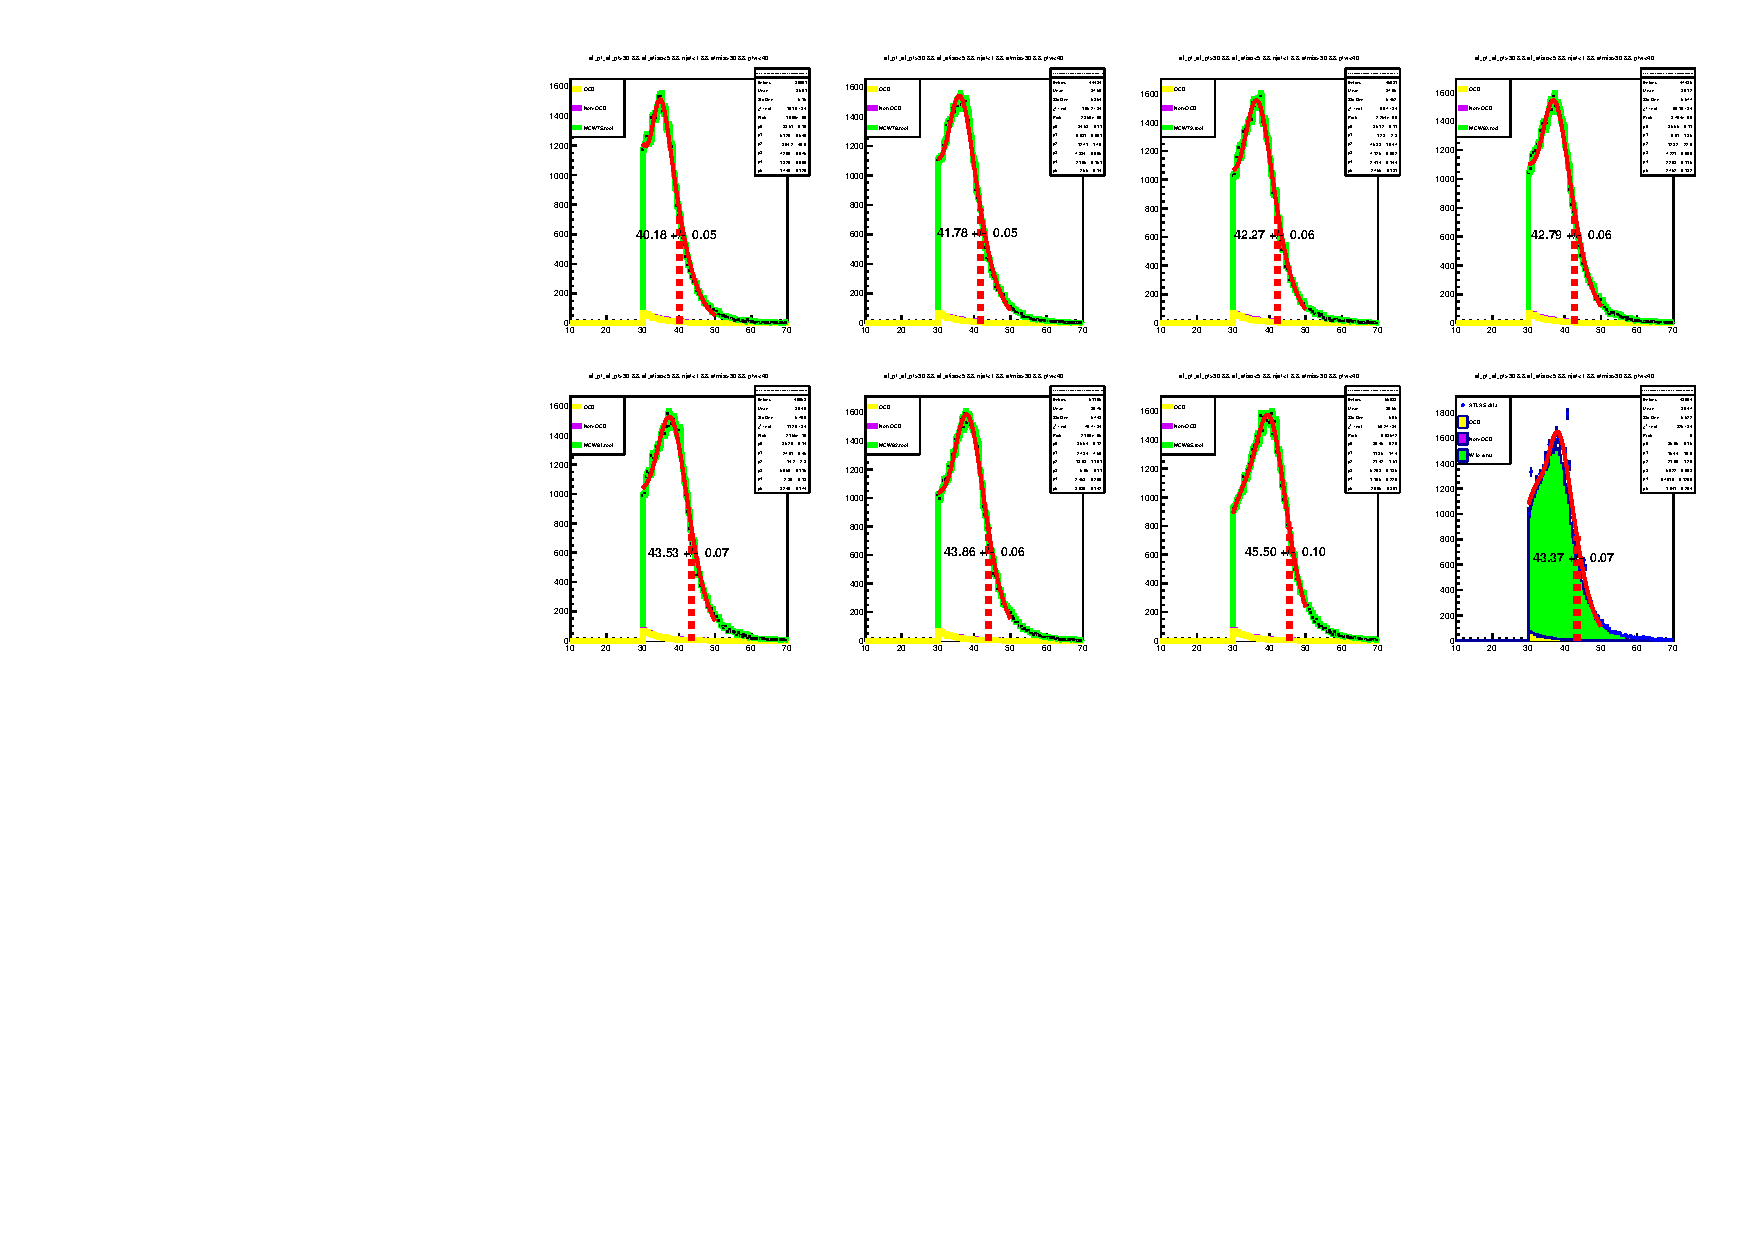
\includegraphics[width=.85\linewidth]{P1_pics/gauge/gauge_curve.pdf}
	\caption{Estimation of the \textsc{Jacobi} peak in the simulated and real data. x-axis: electron $p_t$, y-axis: no. of entries. The order of the simulated datasets corresponds to table \ref{tab:datasets}.}
	\label{fig:gauge_orig}
\end{figure}
\begin{figure}[H]
	\centering
	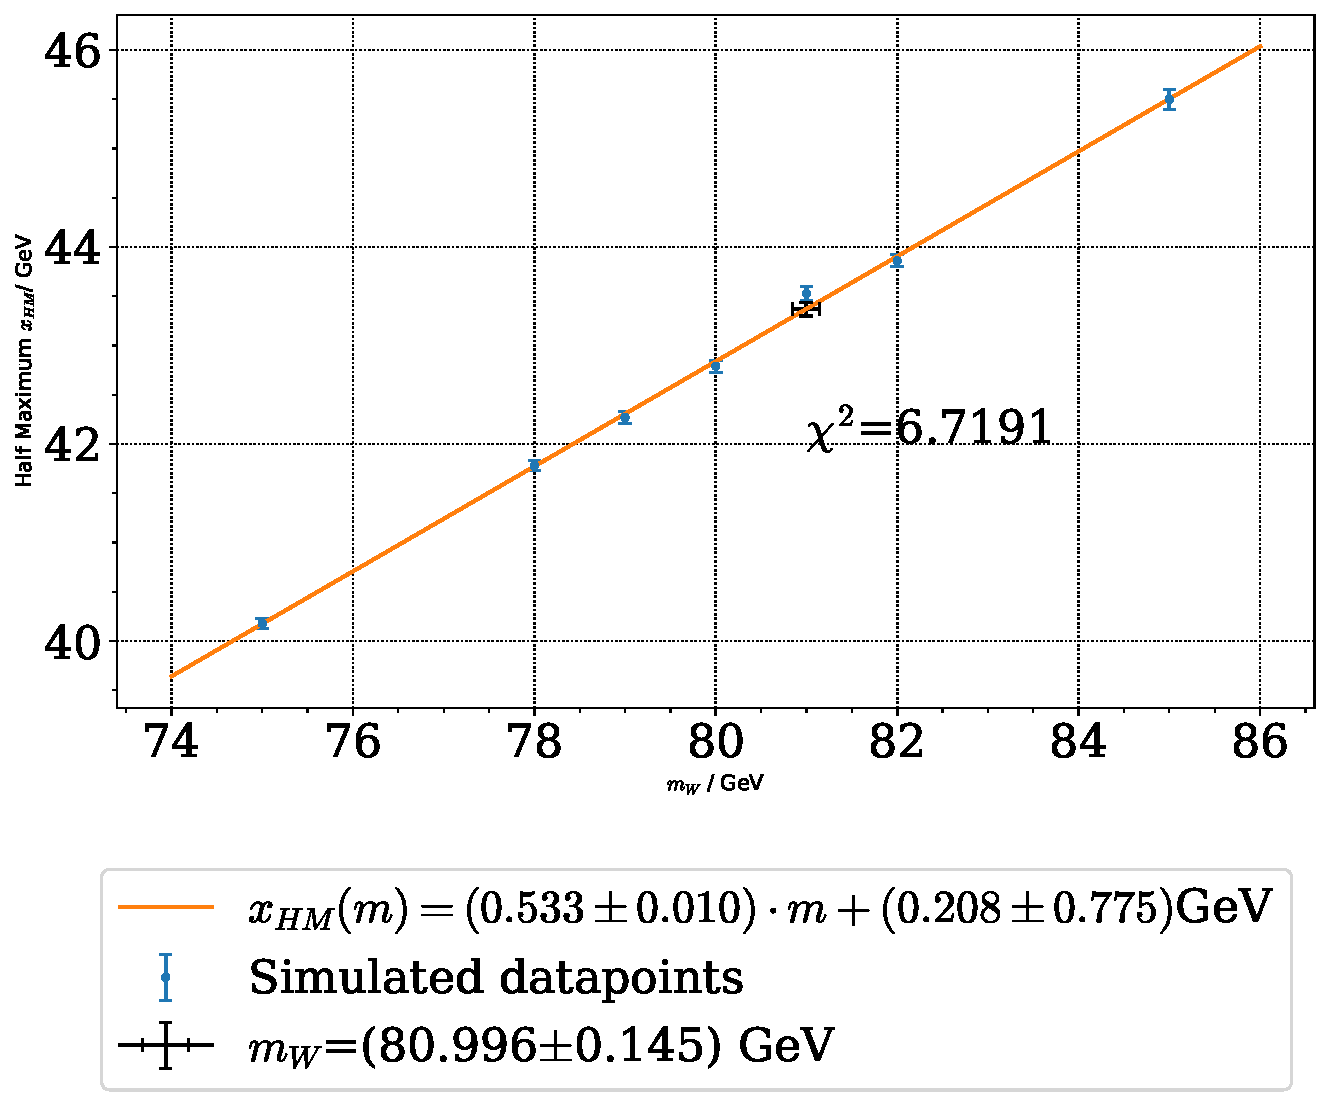
\includegraphics[width=0.65\linewidth]{P1_pics/gauge_results/gauge.pdf}
	\caption{Gauge curve based on simulated data. The mass of the $W$-Boson was extracted from the linear fit by inserting the half-maximum point $x_{\text{HM}}$ of the real ATLAS dataset.}\label{fig:gauge}
\end{figure}







To get the $W$-Boson mass we inserted $x_{\text{HM}}(m_W)$ in the rearranged linear function
\begin{align}\label{eq:m_w_result}
	\begin{split}
			x_{\text{HM}}(m)=a\cdot m+b &\Rightarrow m(x_{\text{HM}})=\frac{x_\text{HM}-b}{a}\\
			x_{\text{HM}}(m_W)=(43.37\pm0.07)\text{ GeV} &\Rightarrow m(x_{\text{HM}})=(80.996\pm0.145)\text{ GeV}.
	\end{split}
\end{align}

\noindent To do the statistical error propagation for the Boson mass $m_W$, we used the \texttt{python}-library \texttt{scipy} which returns the covariant matrix $\sigma$. With this matrix the statistical error can be written as eq. \eqref{eq:err}:

\begin{equation}
	\Delta m_W(x_\text{HM}) = \sqrt{2\cdot\left(\frac{x_{\text{HM}}-b}{a^3}\cdot \sigma_{01}\right)+\left(\frac{1}{a}\Delta x_{\text{HM}}\right)^2+\left(\frac{1}{a}\cdot \Delta b\right)^2+\left(\frac{x_\text{HM}-b}{a^2}\Delta a\right)^2}
\end{equation}
The literature value of the $W$-Boson mass (($80.379 \pm 0.012$) GeV \cite{pdg}) does not lie in the error of the result \ref{eq:m_w_result} yet. We have to include the systematical error.



\subsubsection{Systematic effects and error sources}
To analyse the systematic impact and potential error sources, we modified one parameter at a time, while letting the others be fixated. We then got a slightly different result for the $W$-Boson mass $m_W$ (see \ref{fig:gauge_curve_rest} for all gauge curves). In table \ref{tab:m_mod} are the results listed. Not all parameters got changed, for example the number of jets $n_\text{jet}$. In physical reasoning it would not make sense to look at produced Hadrons while we are detecting the $W\to e\nu$ decay. If the number of jets really would have an influence in a physical manner, the systematic error whouldn't lie in the analysis and rather in the experiment.
\begin{table}[h]
	\centering
	\begin{tabular}{|llll|ll|}\hline
		\multicolumn{4}{|c}{Parameter}                            & \multicolumn{2}{|c|}{$m_{W}$ / GeV}                                             \\
		&                & Min   & Max   & \multicolumn{1}{c}{Min}                                   & \multicolumn{1}{c|}{Max}                                   \\\hline
		$p_t^e$ / GeV          & \textgreater{} & 28    & 32    & $80.808\pm0.144$  & $80.911\pm0.132$  \\
		$\not$$E_t$ / GeV      & \textgreater{} & 28    & 32    & $81.081\pm0.162$  & $81.081\pm0.162$  \\
		$p_t^W$ / GeV          & \textless{}    & 38    & 42    & $81.005\pm0.163$ & $80.981\pm0.166$  \\
		QCD-Scale factor       & =              & 0.317 & 0.375 & $80.984\pm0.145$ & $80.894\pm0.206$ \\
		$E_t^\text{iso}$ / GeV & \textless{}    & 5     & 7     & \multicolumn{2}{c|}{$81.009\pm0.161$}  \\
		$x$ / GeV                   & $\in$              & 25    & 50    & \multicolumn{2}{c|}{$80.996\pm0.145$}                      \\
		$x$ / GeV                    & $\in$              & 25    & 55    & \multicolumn{2}{c|}{$80.934\pm0.109$}                     \\
		$x$ / GeV              & $\in$              & 30    & 55    & \multicolumn{2}{c|}{$80.937\pm0.110$}\\\hline                               
	\end{tabular}
\caption{$W$-Boson mass results with different parameter limits. All other parameters were fixed.}\label{tab:m_mod}
\end{table}

To get the systematic error, we calculated the difference between the result \ref{eq:m_w_result} and the partial results from table \ref{tab:m_mod}. By summing up all negative and positive spreads, we find the systematic error:
\begin{equation}
	m_W=m_W^\text{stat.}+\Delta m_W^\text{stat.}+\Delta m_W^\text{syst.}=\left(80.996\pm0.145+^{+0.193}_{-0.595}\right)\text{GeV}
\end{equation}
The literature value $(80.379 \pm 0.012)$ GeV \cite{pdg} lies now in the error. 


This ansatz only gives an estimate of the systematic error because it presupposes that all parameters are independent. This surely isn't the case, especially for the momenta. One could iterate over all combinations and with smaller steps to find a more suitable result. We hadn't the time to do so, because such calculations can take up to hours and even days. We were also not that proficient in \texttt{root} automatisation.



An additional way to inspect the systematic error is to take a look at the $Z\to e⁺e⁻$ decay. This offers a good opportunity because we calibrated the experiment with this decay and especially with the literature value of the the $Z$-Boson. If the mass of the $Z$-Boson $m_Z$ differs from the literature value --what should be a calibration error-- one could find a correction factor. Figure \ref{fig:m_Z} shows the gauge curve for the $Z$-Boson and figure \ref{fig:p_Z} the $p_t$-spectrum of the $Z\to e^+e^-$ decay. The result of this measurement is 
$$m_Z=(90.375\pm0.855)\text{GeV}.$$
\begin{figure}[h]
	\centering
	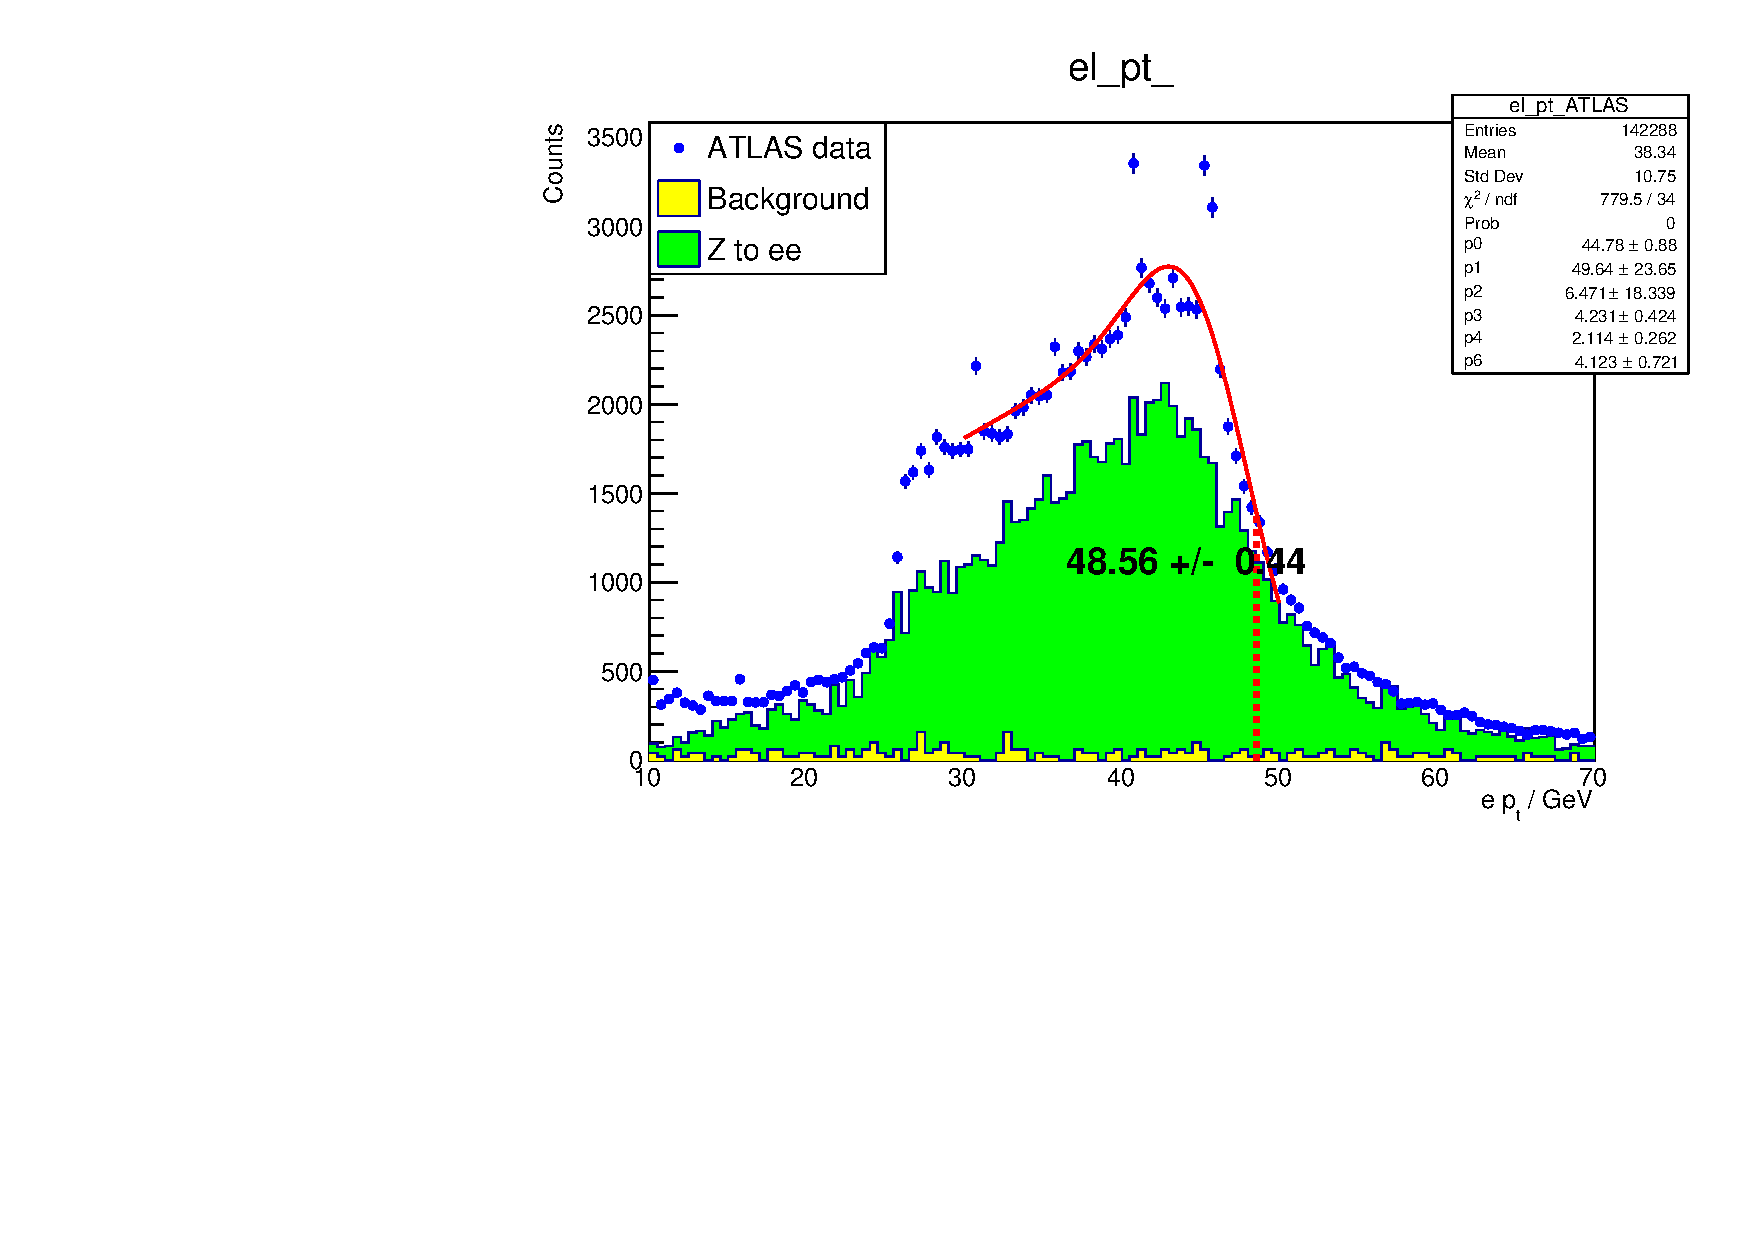
\includegraphics[width=0.7\linewidth]{P1_pics/gauge/Zee_HM.pdf}
	\caption{$p_t$ spectrum of the $Z\to e^+e^-$ decay}\label{fig:p_Z}
\end{figure} 

\begin{figure}[h]
	\centering
	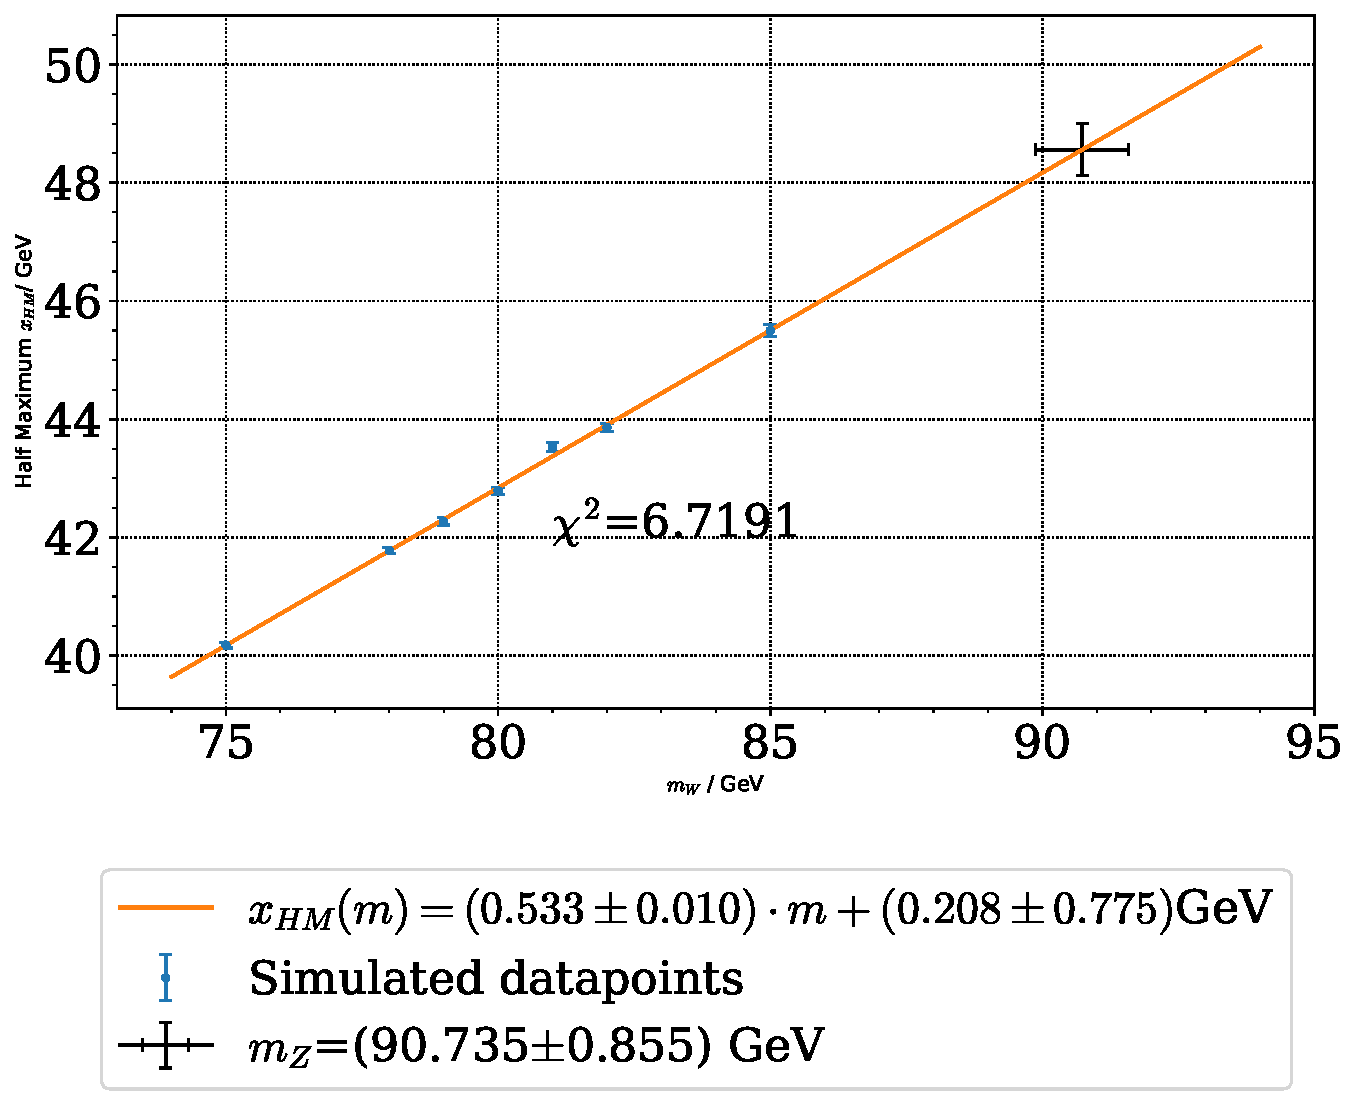
\includegraphics[width=0.7\linewidth]{P1_pics/gauge_results/Zee.pdf}
	\caption{Gauge curve to find the $Z$-Boson mass $m_Z$}\label{fig:m_Z}
\end{figure} 

For this the literature value $m_Z=(91.1876\pm 0.0021)$ GeV is included in the error of our measurement. 

This result does not lead to a conclusion of a faulty calibration, since other systematic errors, like parameter cuts could have a significant impact on the result. While doing the experiment, applying cuts and QCD-factors didn't work for the \texttt{Zee} dataset. This is also the reason, why the stack plot isn't matching the ATLAS data in figure \ref{fig:p_Z}. Because of this we couldn't find a systematic error like before for this dataset. 

The statistic error of the $Z$-Boson mass is also rather high in comparison to the $W$-Boson mass (factor of about 5). This is an interesting side note, because one would expect, that the error of the $Z$-Boson mass would be at least as small as for the $W$-Boson because of calibration purposes. On the other hand the half maximum was found with uncut data resulting in a larger error of this quantity which of course propagates.

By revisiting the experiment, one could fix those problems and take more data for the systematic error prediction. But at this point it would break the boundaries of the lab course. The result of this section leads to the conclusion, that the calibration can have a significant impact on the result as well as the cut selection and the QCD-factor. All variables should be chosen wisely and should be also investigated on their systematic behaviour. Not only for this reason one can get directly pre calibrated datasets from the ATLAS group.

\newpage

\section{Conclusion}
In this lab course we investigated hadron collisions done at the ATLAS experiment. We calibrated the detector and analysed real world data with the help of simulations and the use of graphical event viewing software.

We began to visually investigate the trajectories of leptons --namely electrons, myons and tauons--, photons and also of hadron jets in the event viewing software \texttt{ATLANTIS}. After getting used to the software we also measured the energy and the momenta of 20 electrons and calculated the ratio $\beta=\frac{p}{E}$ and created a histogram from it. 
After that we measured the energy and momentum of three possible electron positron pairs, which originated from the decay of a $Z$-Boson. The goal was to reproduce the $Z$ mass. This wasn't unfortunately possible due to faulty measurements.

Next we calibrated the electromagnetic calorimeter by using the $Z\to e^+e^-$ decay and the well known mass $m_Z$. We only iterated the calibration once, because more iterations resulted in worse results for the mass $m_Z$ as well as the detector resolution
\begin{align*}
	m_Z^{\text{calib}}=\SI{91.22\pm0.02}{\giga\eV} && \Delta^\text{calib}=\SI{2.281\pm0.024}{\giga\eV}.
\end{align*}

To measure the $W$-Boson mass we searched for proper cut selections and a QCD-scale factor. With parameters set, we then used simulated data to create a gauge curve from the so called half-maximum point of the \textsc{Jacobi} peak in the $p_t$-spectrum of the electron. We also measured the half-maximum point in a real ATLAS dataset. With a linear fit, we then could derive the $W$-Boson mass with a statistic error.

Since the statistic error was rather small and the literature value of the $W$-Boson wasn't yet included we took a look at the systematic errors. By varying one parameter and keeping the others fixed we estimated a systematic error. This first estimate ignores the dependence of parameters on each other. But since the computation time would take to long for the lab course, we skipped a more precise iterative ansatz. Nevertheless the literature value of the $W$-Boson mass is included in the error now.

Our result for the $W$-mass is
$$	m_W=m_W^\text{stat.}+\Delta m_W^\text{stat.}+\Delta m_W^\text{syst.}=\left(80.996\pm0.145+^{+0.193}_{-0.595}\right)\text{GeV}$$
which is for the used approach a fairly good result.

Last we measured the $Z$-Boson mass by the same method.
$$m_Z=(90.375\pm0.855)\text{GeV}$$
The literature value lies in the statistical error of this measurement giving no need to include further systematic errors on the $W^\pm$ mass. 

One could investigate in a follow up the systematic impact even more precisely and look further in the quality and the effects of the calibration and cut selection.    
\label{sec:conc}
\newpage
\appendix\section{Appendix}\label{sec:Appendix}
\counterwithin{figure}{section}

\subsection*{Calibration}
Our calibration is also available for download on our \hyperref{https://github.com/krausejm/advanced_lab_course}{}{}{GitHub-Repository}.
\lstset{language=C}
\begin{lstlisting}[numbers=left, breaklines=true]
#include "math.h"
#include "TMath.h"

double ElecCalib(double e_raw, double pt, double eta, 
double phi, double etiso, double eoverp, double mindrjet)
{
	double dummy=pt*eta*phi*etiso*eoverp*mindrjet;
	double z_mass = 91.1876;
	double energy = e_raw;
	if ((eta)<-2.4) energy = energy * z_mass/86.27;
	else if (eta<-2.3 && eta>=-2.4) energy = energy * z_mass/87.11;
	else if (eta<-2.2 && eta>=-2.3) energy = energy * z_mass/87.64;
	else if (eta<-2.1 && eta>=-2.2) energy = energy * z_mass/88.42;
	else if (eta<-2.0 && eta>=-2.1) energy = energy * z_mass/89.30;
	else if (eta<-1.9 && eta>=-2.0) energy = energy * z_mass/89.44;
	else if (eta<-1.8 && eta>=-1.9) energy = energy * z_mass/89.55;
	else if (eta<-1.7 && eta>=-1.8) energy = energy * z_mass/90.25;
	else if (eta<-1.6 && eta>=-1.7) energy = energy * z_mass/88.73;
	else if (eta<-1.5 && eta>=-1.6) energy = energy * z_mass/89.42;
	else if (eta<-1.4 && eta>=-1.5) energy = energy * z_mass/87.31;
	else if (eta<-1.3 && eta>=-1.4) energy = energy * z_mass/89.53;
	else if (eta<-1.2 && eta>=-1.3) energy = energy * z_mass/89.44;
	else if (eta<-1.1 && eta>=-1.2) energy = energy * z_mass/89.26;
	else if (eta<-1.0 && eta>=-1.1) energy = energy * z_mass/89.58;
	else if (eta<-0.9 && eta>=-1.0) energy = energy * z_mass/89.08;
	else if (eta<-0.8 && eta>=-0.9) energy = energy * z_mass/89.56;
	else if (eta<-0.7 && eta>=-0.8) energy = energy * z_mass/89.54;
	else if (eta<-0.6 && eta>=-0.7) energy = energy * z_mass/89.82;
	else if (eta<-0.5 && eta>=-0.6) energy = energy * z_mass/89.82;
	else if (eta<-0.4 && eta>=-0.5) energy = energy * z_mass/90.20;
	else if (eta<-0.3 && eta>=-0.4) energy = energy * z_mass/89.88;
	else if (eta<-0.2 && eta>=-0.3) energy = energy * z_mass/90.06;
	else if (eta<-0.1 && eta>=-0.2) energy = energy * z_mass/89.82;
	else if (eta<-0.0 && eta>=-0.1) energy = energy * z_mass/89.98;
	else if (eta>=0.0 && eta<0.1) energy = energy * z_mass/89.78;
	else if (eta>=0.1 && eta<0.2) energy = energy * z_mass/89.99;
	else if (eta>=0.2 && eta<0.3) energy = energy * z_mass/89.92;
	else if (eta>=0.3 && eta<0.4) energy = energy * z_mass/89.83;
	else if (eta>=0.4 && eta<0.5) energy = energy * z_mass/89.96;
	else if (eta>=0.5 && eta<0.6) energy = energy * z_mass/89.9;
	else if (eta>=0.6 && eta<0.7) energy = energy * z_mass/89.72;
	else if (eta>=0.7 && eta<0.8) energy = energy * z_mass/89.59;
	else if (eta>=0.8 && eta<0.9) energy = energy * z_mass/89.33;
	else if (eta>=0.9 && eta<1.0) energy = energy * z_mass/89.39;
	else if (eta>=1.0 && eta<1.1) energy = energy * z_mass/89.30;
	else if (eta>=1.1 && eta<1.2) energy = energy * z_mass/89.49;
	else if (eta>=1.2 && eta<1.3) energy = energy * z_mass/89.04;
	else if (eta>=1.3 && eta<1.4) energy = energy * z_mass/89.81;
	else if (eta>=1.4 && eta<1.5) energy = energy * z_mass/89.06;
	else if (eta>=1.5 && eta<1.6) energy = energy * z_mass/89.1;
	else if (eta>=1.6 && eta<1.7) energy = energy * z_mass/88.7;
	else if (eta>=1.7 && eta<1.8) energy = energy * z_mass/90.12;
	else if (eta>=1.8 && eta<1.9) energy = energy * z_mass/90.1;
	else if (eta>=1.9 && eta<2.0) energy = energy * z_mass/89.6;
	else if (eta>=2.0 && eta<2.1) energy = energy * z_mass/88.96;
	else if (eta>=2.1 && eta<2.2) energy = energy * z_mass/88.5;
	else if (eta>=2.2 && eta<2.3) energy = energy * z_mass/87.5;
	else if (eta>=2.3 && eta<2.4) energy = energy * z_mass/87.36;
	else if (eta>=2.4 && eta<2.5) energy = energy * z_mass/88.0;
	
	
	
	if((phi)<-3.14*11/12) energy = energy * z_mass/90.85;
	else if (phi>=-3.14*11/12 && phi<-3.14*10/12) energy = energy * z_mass/91.4;
	else if (phi>=-3.14*10/12 && phi<-3.14*9/12) energy = energy * z_mass/91.22;
	else if (phi>=-3.14*9/12 && phi<-3.14*8/12) energy = energy * z_mass/91.1;
	else if (phi>=-3.14*8/12 && phi<-3.14*7/12) energy = energy * z_mass/91.08;
	else if (phi>=-3.14*7/12 && phi<-3.14*6/12) energy = energy * z_mass/91.08;
	else if (phi>=-3.14*6/12 && phi<-3.14*5/12) energy = energy * z_mass/91.29;
	else if (phi>=-3.14*5/12 && phi<-3.14*4/12) energy = energy * z_mass/91.33;
	else if (phi>=-3.14*4/12 && phi<-3.14*3/12) energy = energy * z_mass/90.91;
	else if (phi>=-3.14*3/12 && phi<-3.14*2/12) energy = energy * z_mass/91.19;
	else if (phi>=-3.14*2/12 && phi<-3.14*1/12) energy = energy * z_mass/91.4;
	else if (phi>=-3.14*1/12 && phi<-3.14*0/12) energy = energy * z_mass/90.92;
	else if (phi>=-3.14*0/12 && phi<+3.14*1/12) energy = energy * z_mass/90.84;
	else if (phi>=3.14*1/12 && phi<+3.14*2/12) energy = energy * z_mass/91.19;
	else if (phi>=3.14*2/12 && phi<+3.14*3/12) energy = energy * z_mass/91.4;
	else if (phi>=3.14*3/12 && phi<+3.14*4/12) energy = energy * z_mass/91.11;
	else if (phi>=3.14*4/12 && phi<+3.14*5/12) energy = energy * z_mass/91.32;
	else if (phi>=3.14*5/12 && phi<+3.14*6/12) energy = energy * z_mass/91.13;
	else if (phi>=3.14*6/12 && phi<+3.14*7/12) energy = energy * z_mass/91.17;
	else if (phi>=3.14*7/12 && phi<+3.14*8/12) energy = energy * z_mass/91.18;
	else if (phi>=3.14*8/12 && phi<+3.14*9/12) energy = energy * z_mass/91.09;
	else if (phi>=3.14*9/12 && phi<+3.14*10/12) energy = energy * z_mass/91.16;
	else if (phi>=3.14*10/12 && phi<+3.14*11/12) energy = energy * z_mass/91.43;
	else if (phi>=3.14*11/12) energy = energy * z_mass/90.81;
	
	if(pt<15) energy = energy * z_mass/88.63;
	else if (pt>=3*5 && pt < 4*5) energy = energy * z_mass/90.19;
	else if (pt>=4*5 && pt < 5*5) energy = energy * z_mass/90.47;
	else if (pt>=5*5 && pt < 6*5) energy = energy * z_mass/90.09;
	else if (pt>=6*5 && pt < 7*5) energy = energy * z_mass/90.62;
	else if (pt>=7*5 && pt < 8*5) energy = energy * z_mass/90.75;
	else if (pt>=8*5 && pt < 9*5) energy = energy * z_mass/91.32;
	else if (pt>=9*5 && pt < 10*5) energy = energy * z_mass/92.26;
	else if (pt>=10*5 && pt < 11*5) energy = energy * z_mass/92.14;
	else if (pt>=11*5 && pt < 12*5) energy = energy * z_mass/92.09;
	else if (pt>=12*5 && pt < 13*5) energy = energy * z_mass/91.96;
	else if (pt>=13*5 && pt < 14*5) energy = energy * z_mass/91.81;
	else if (pt>=14*5 && pt < 16*5) energy = energy * z_mass/91.85;
	else if (pt>=16*5) energy = energy * z_mass/91.92;
	
	return energy;
} 
\end{lstlisting}


\subsection*{Figures}
\begin{figure}[H]
	\centering
	\begin{subfigure}{0.49\linewidth}
		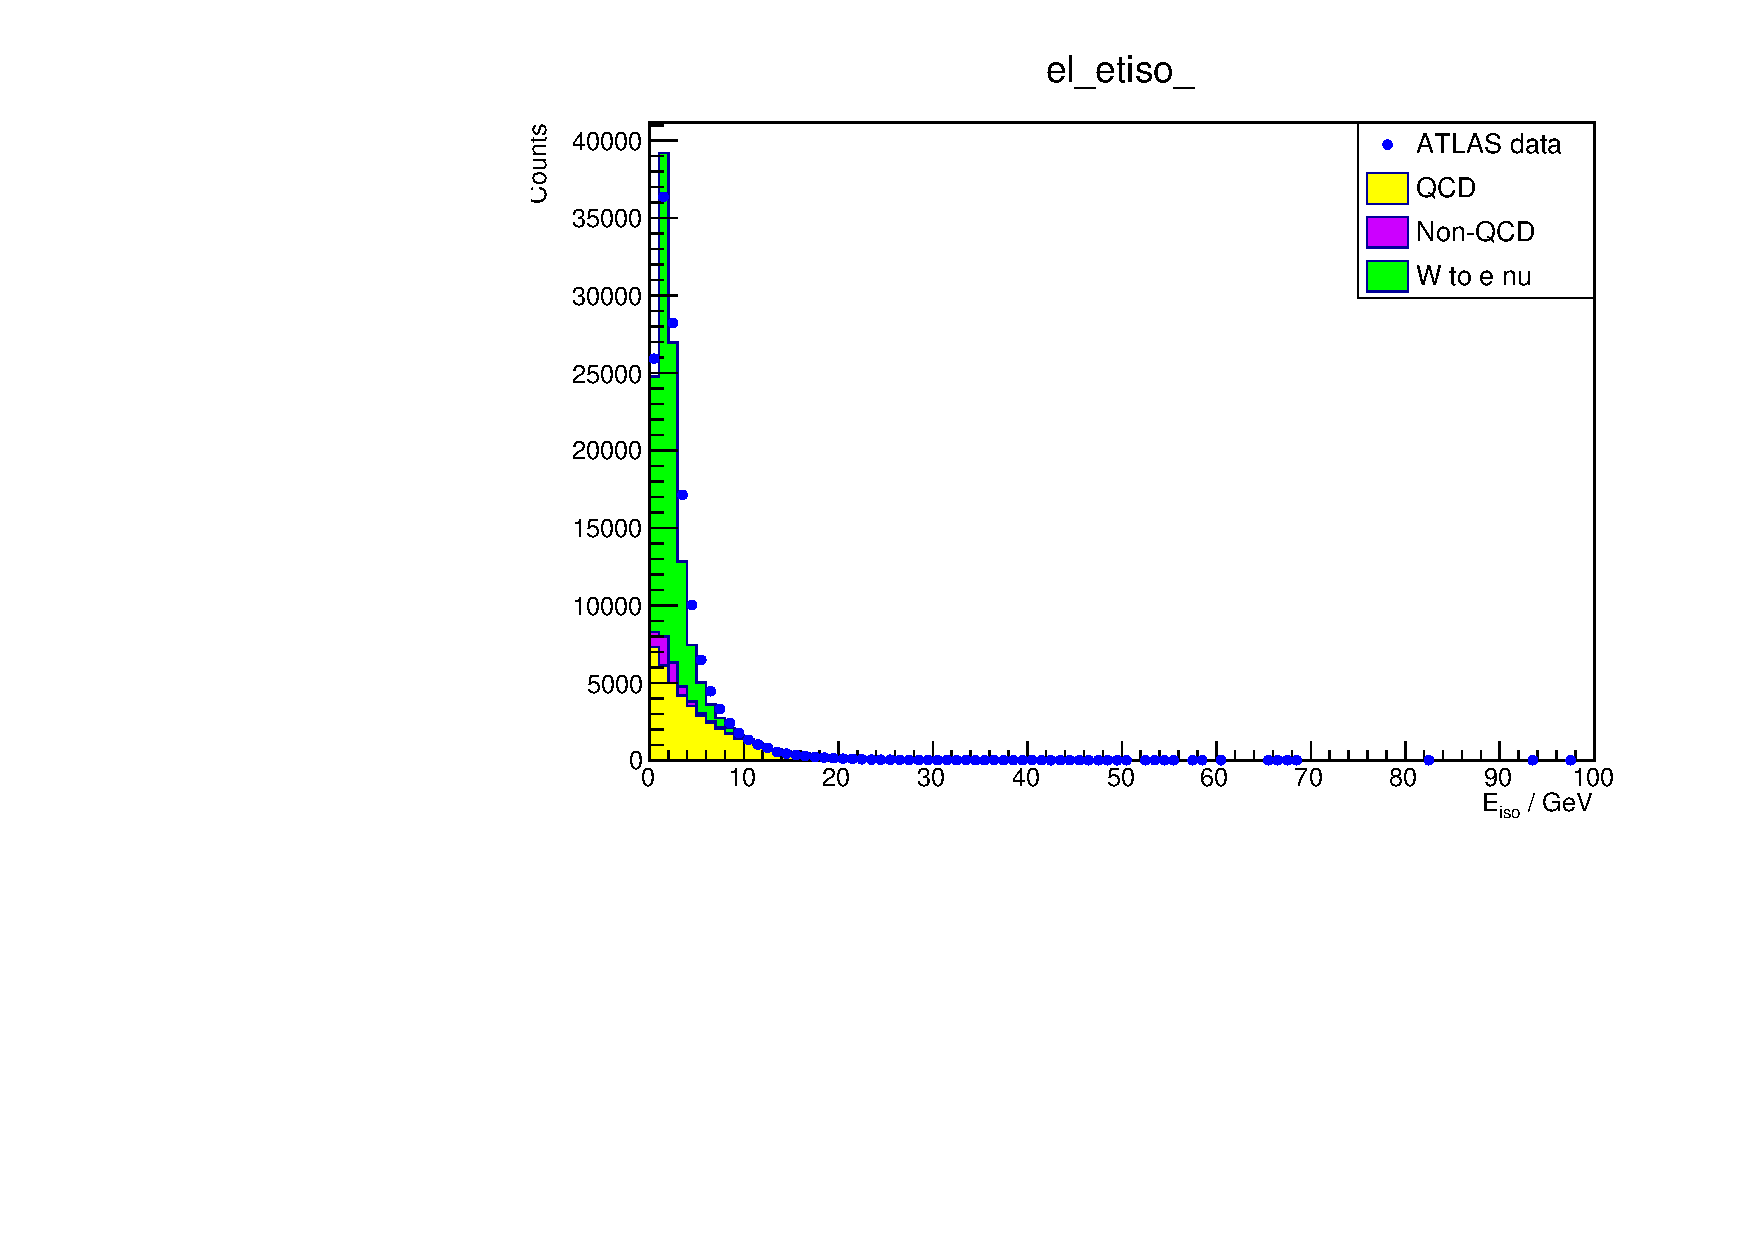
\includegraphics[width=\linewidth]{P1_pics/cuts/el_etiso_qcd_eyeball.pdf}
		\caption{}
	\end{subfigure}
	\begin{subfigure}{0.49\linewidth}
		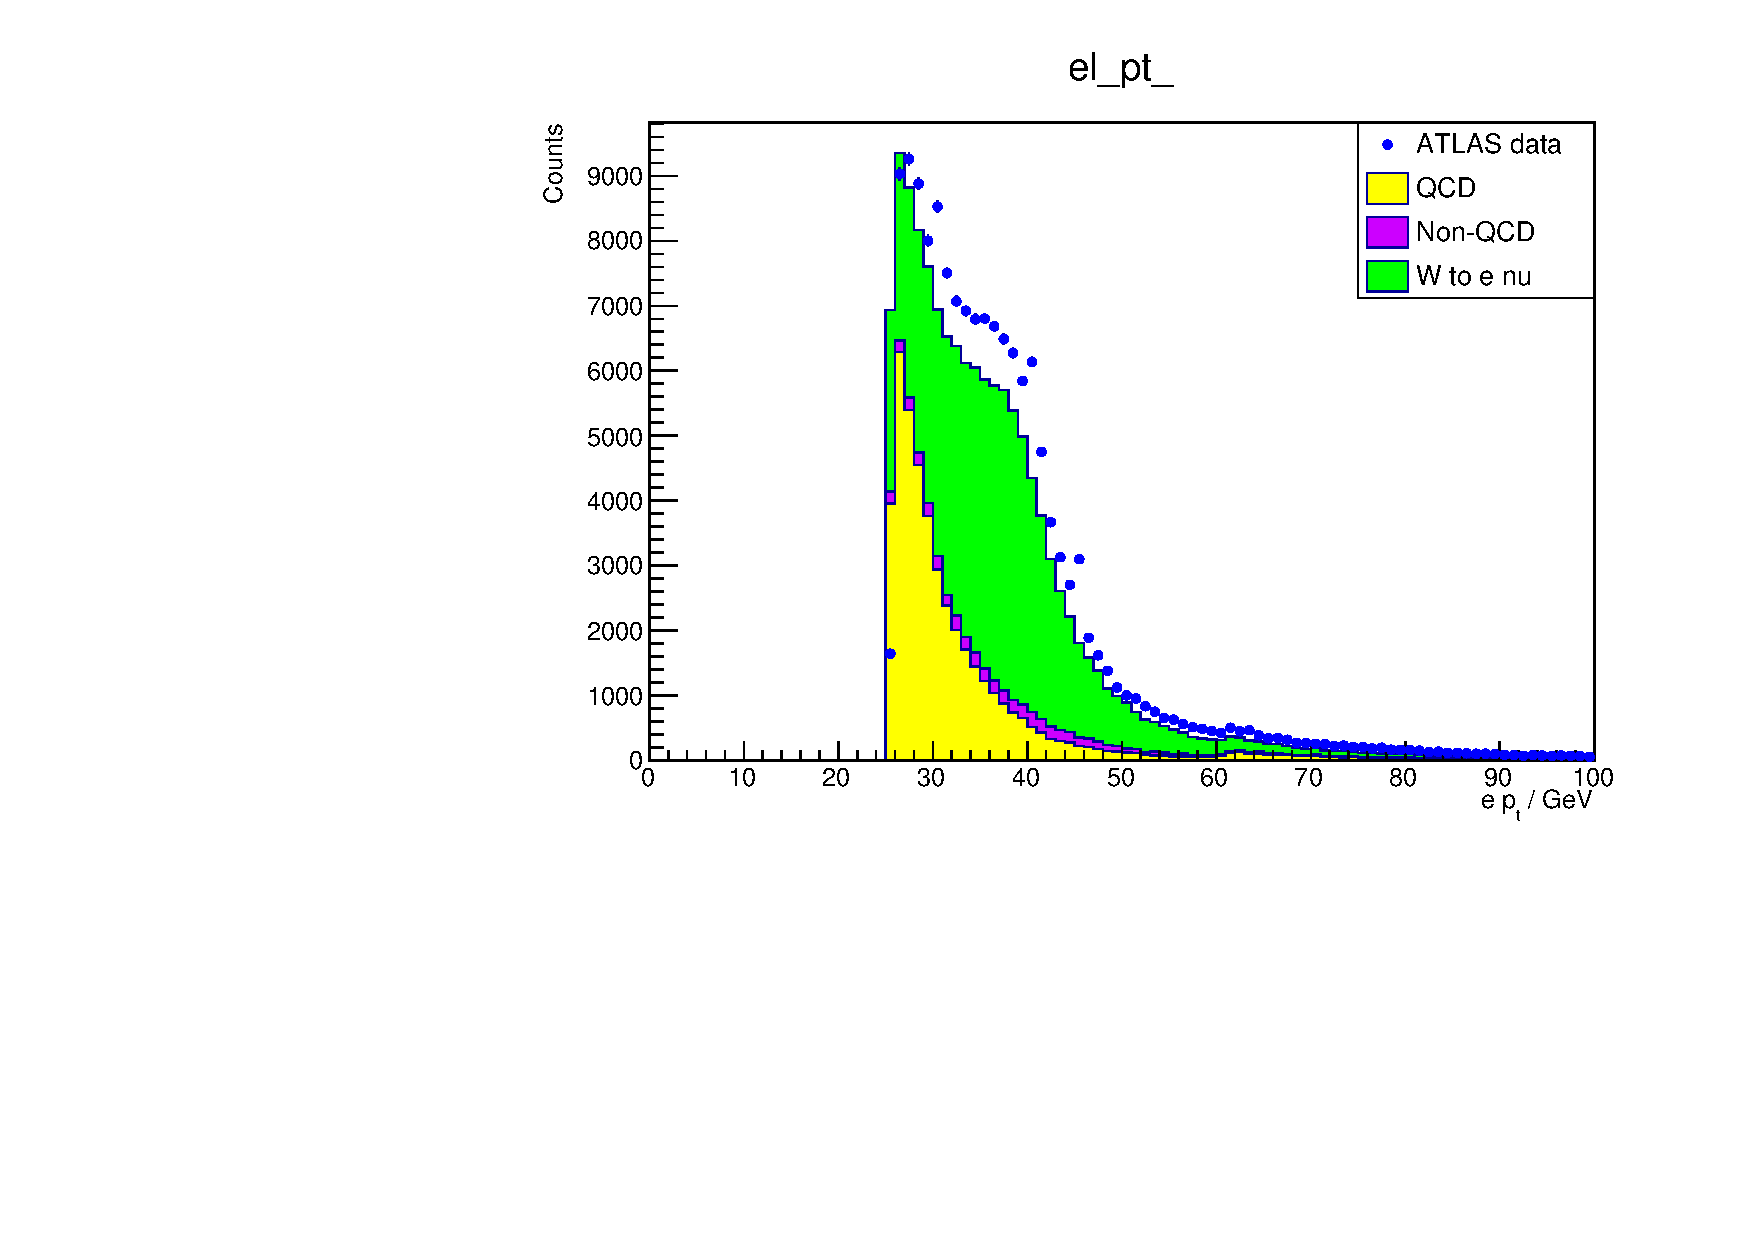
\includegraphics[width=\linewidth]{P1_pics/cuts/el_pt_qcd_eyeball.pdf}
		\caption{}
	\end{subfigure}
	\begin{subfigure}{0.49\linewidth}
		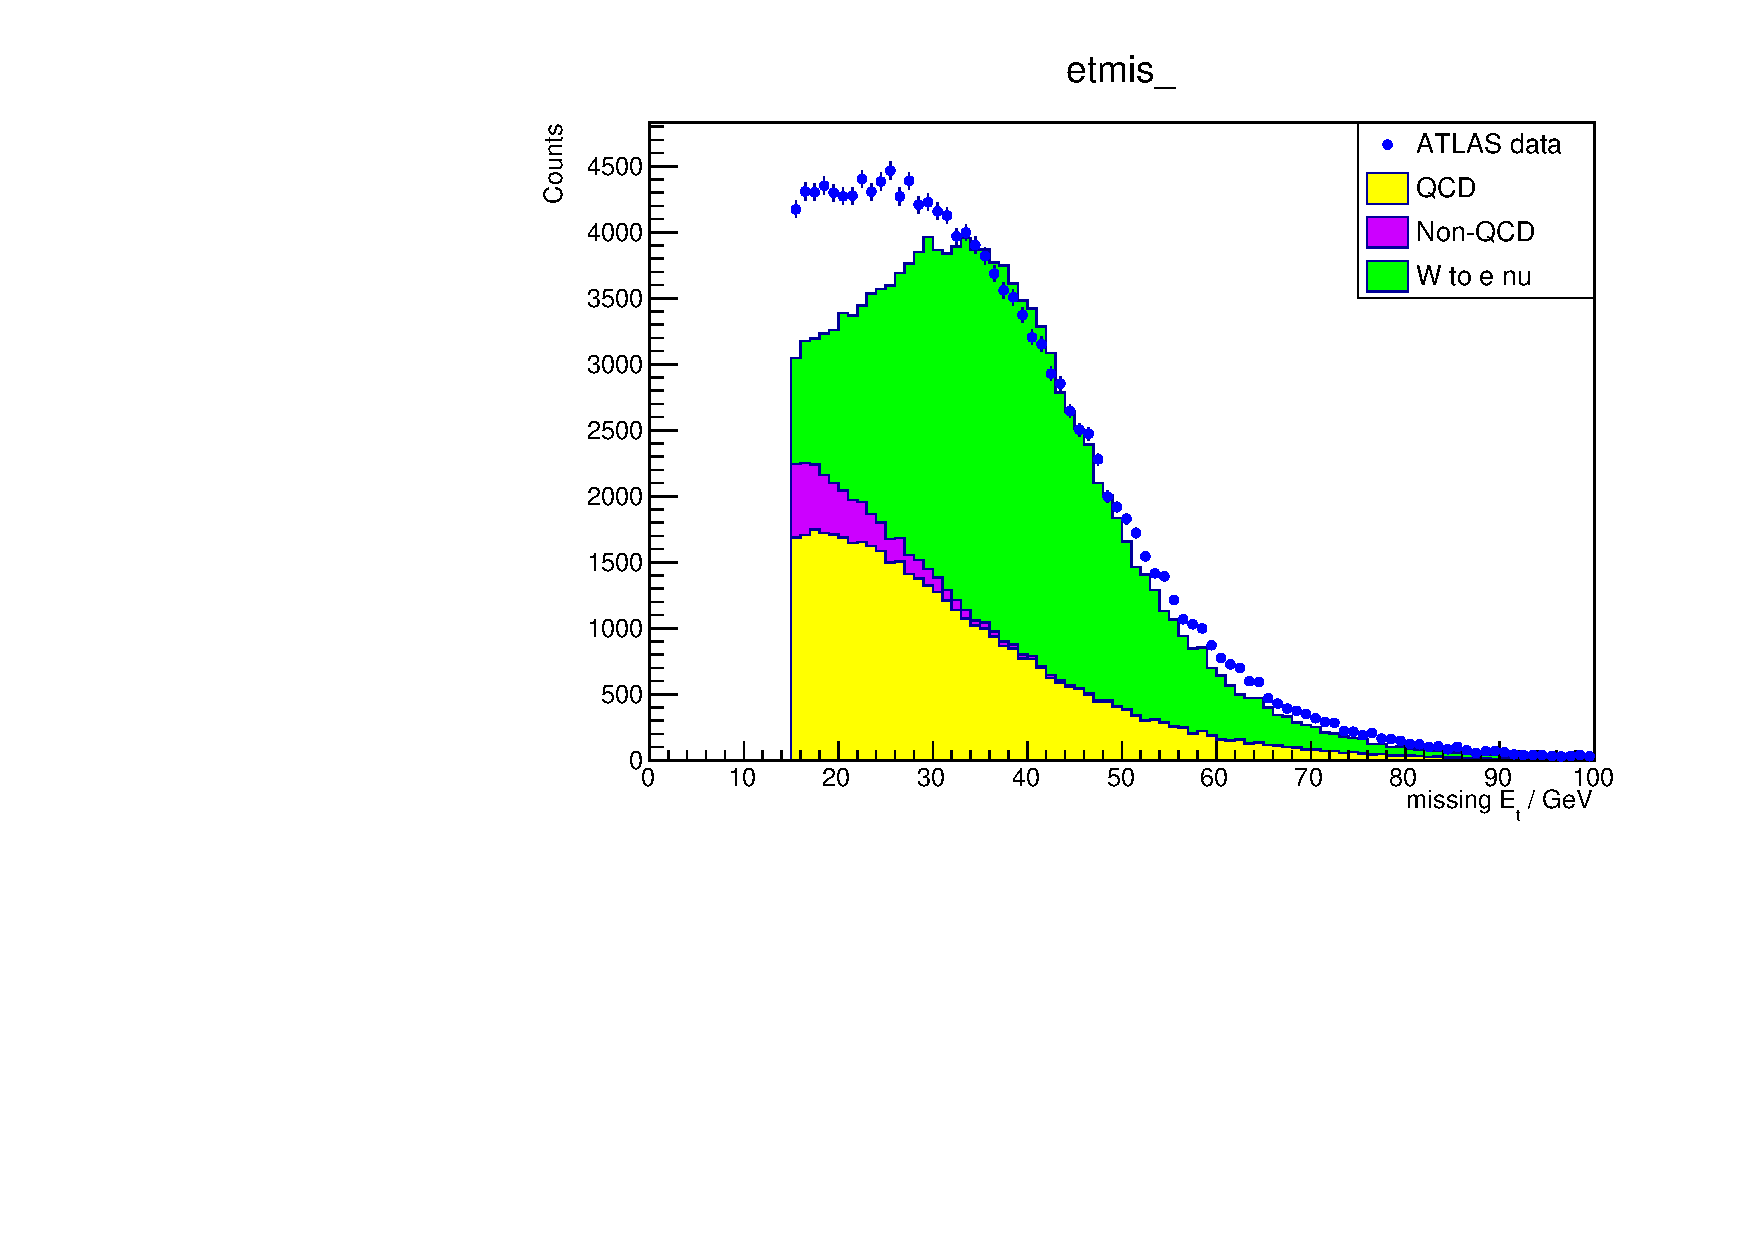
\includegraphics[width=\linewidth]{P1_pics/cuts/etmis_qcd_eyeball.pdf}
		\caption{}
	\end{subfigure}
	\begin{subfigure}{0.49\linewidth}
		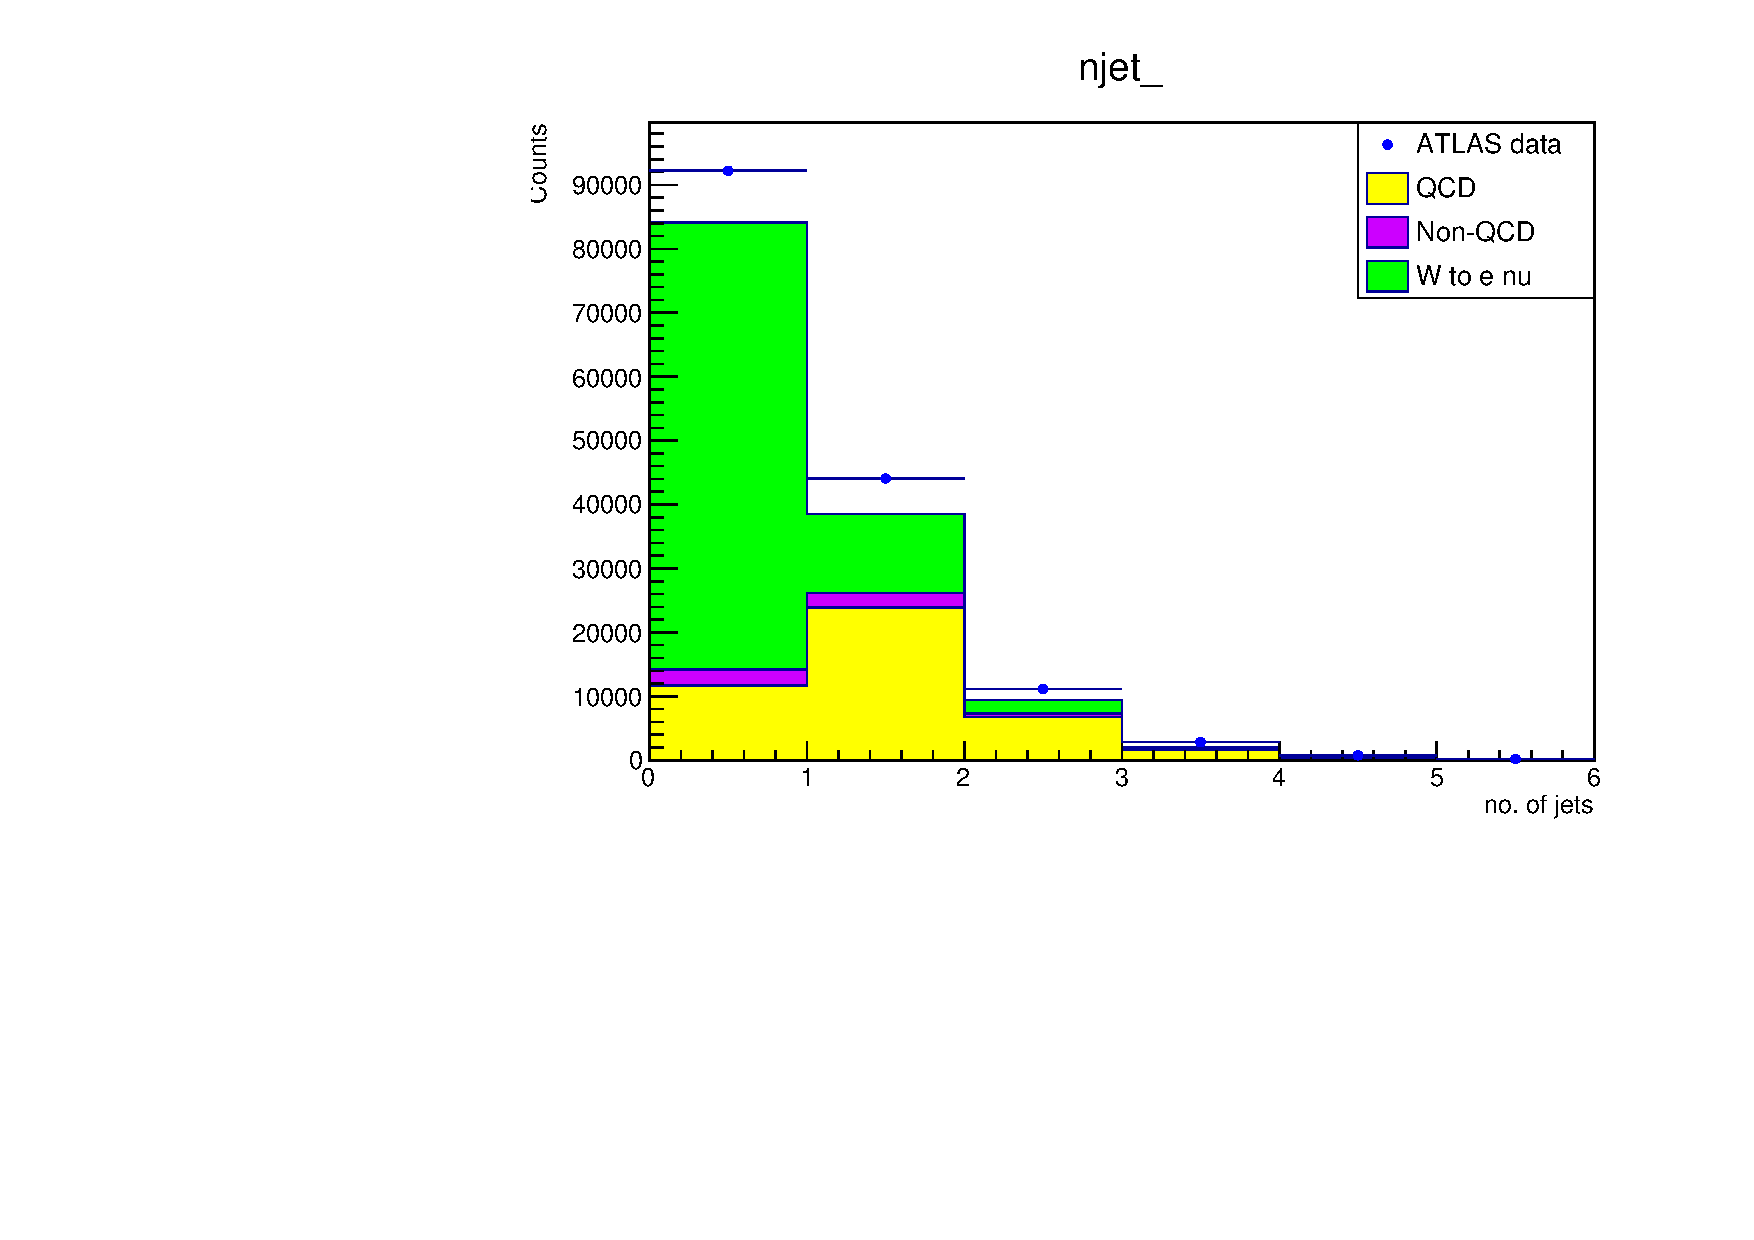
\includegraphics[width=\linewidth]{P1_pics/cuts/njet_qcd_eyeball.pdf}
		\caption{}
	\end{subfigure}
	\begin{subfigure}{0.49\linewidth}
		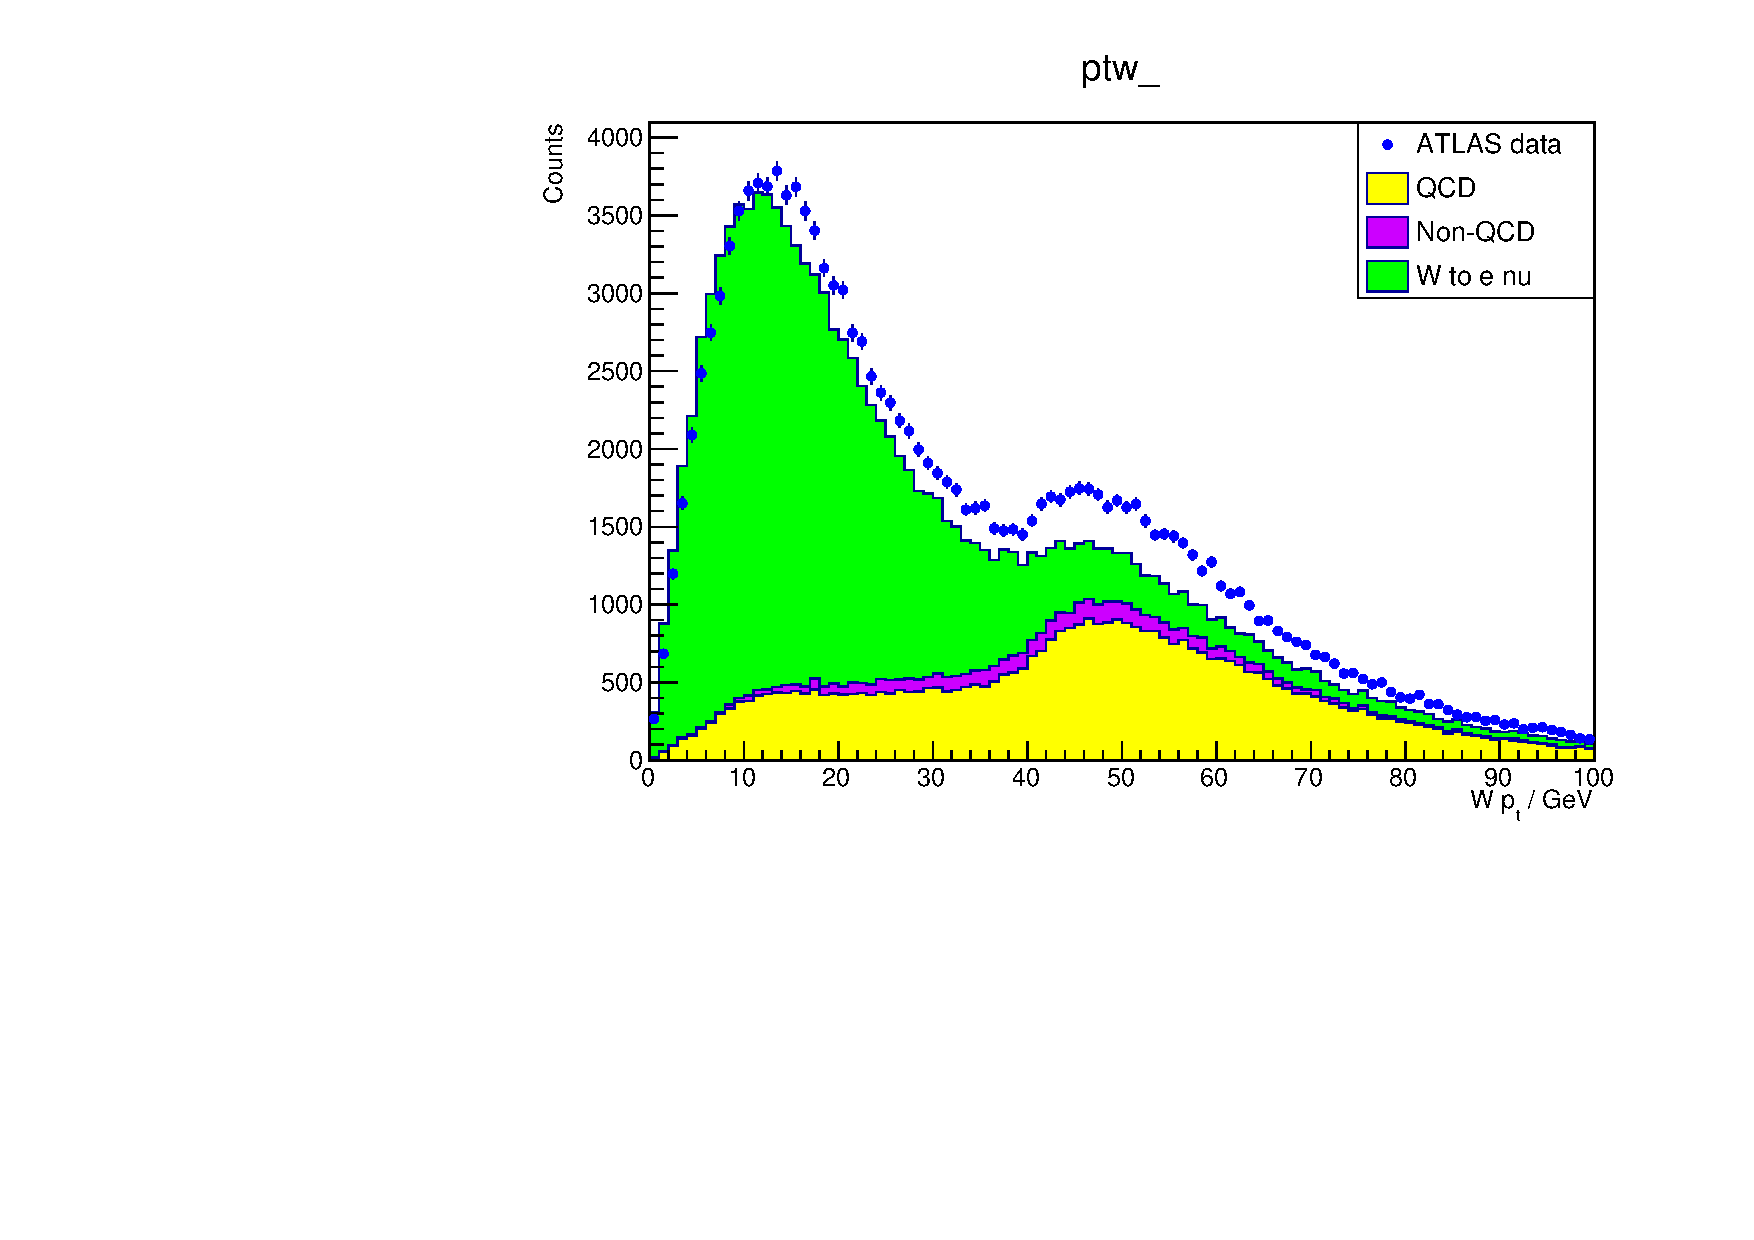
\includegraphics[width=\linewidth]{P1_pics/cuts/ptw_qcd_eyeball.pdf}
		\caption{}
	\end{subfigure}
	\caption{First estimate of the QCD-factor by eye (QCD-factor = $0.3$) for the occurring properties. ATLAS data (blue), simulated $Z\to ee$ decay events (green) and background (yellow)}\label{fig:eyeballed_cuts}
\end{figure}
\begin{figure}[H]
	\centering
	\begin{subfigure}{0.49\linewidth}
		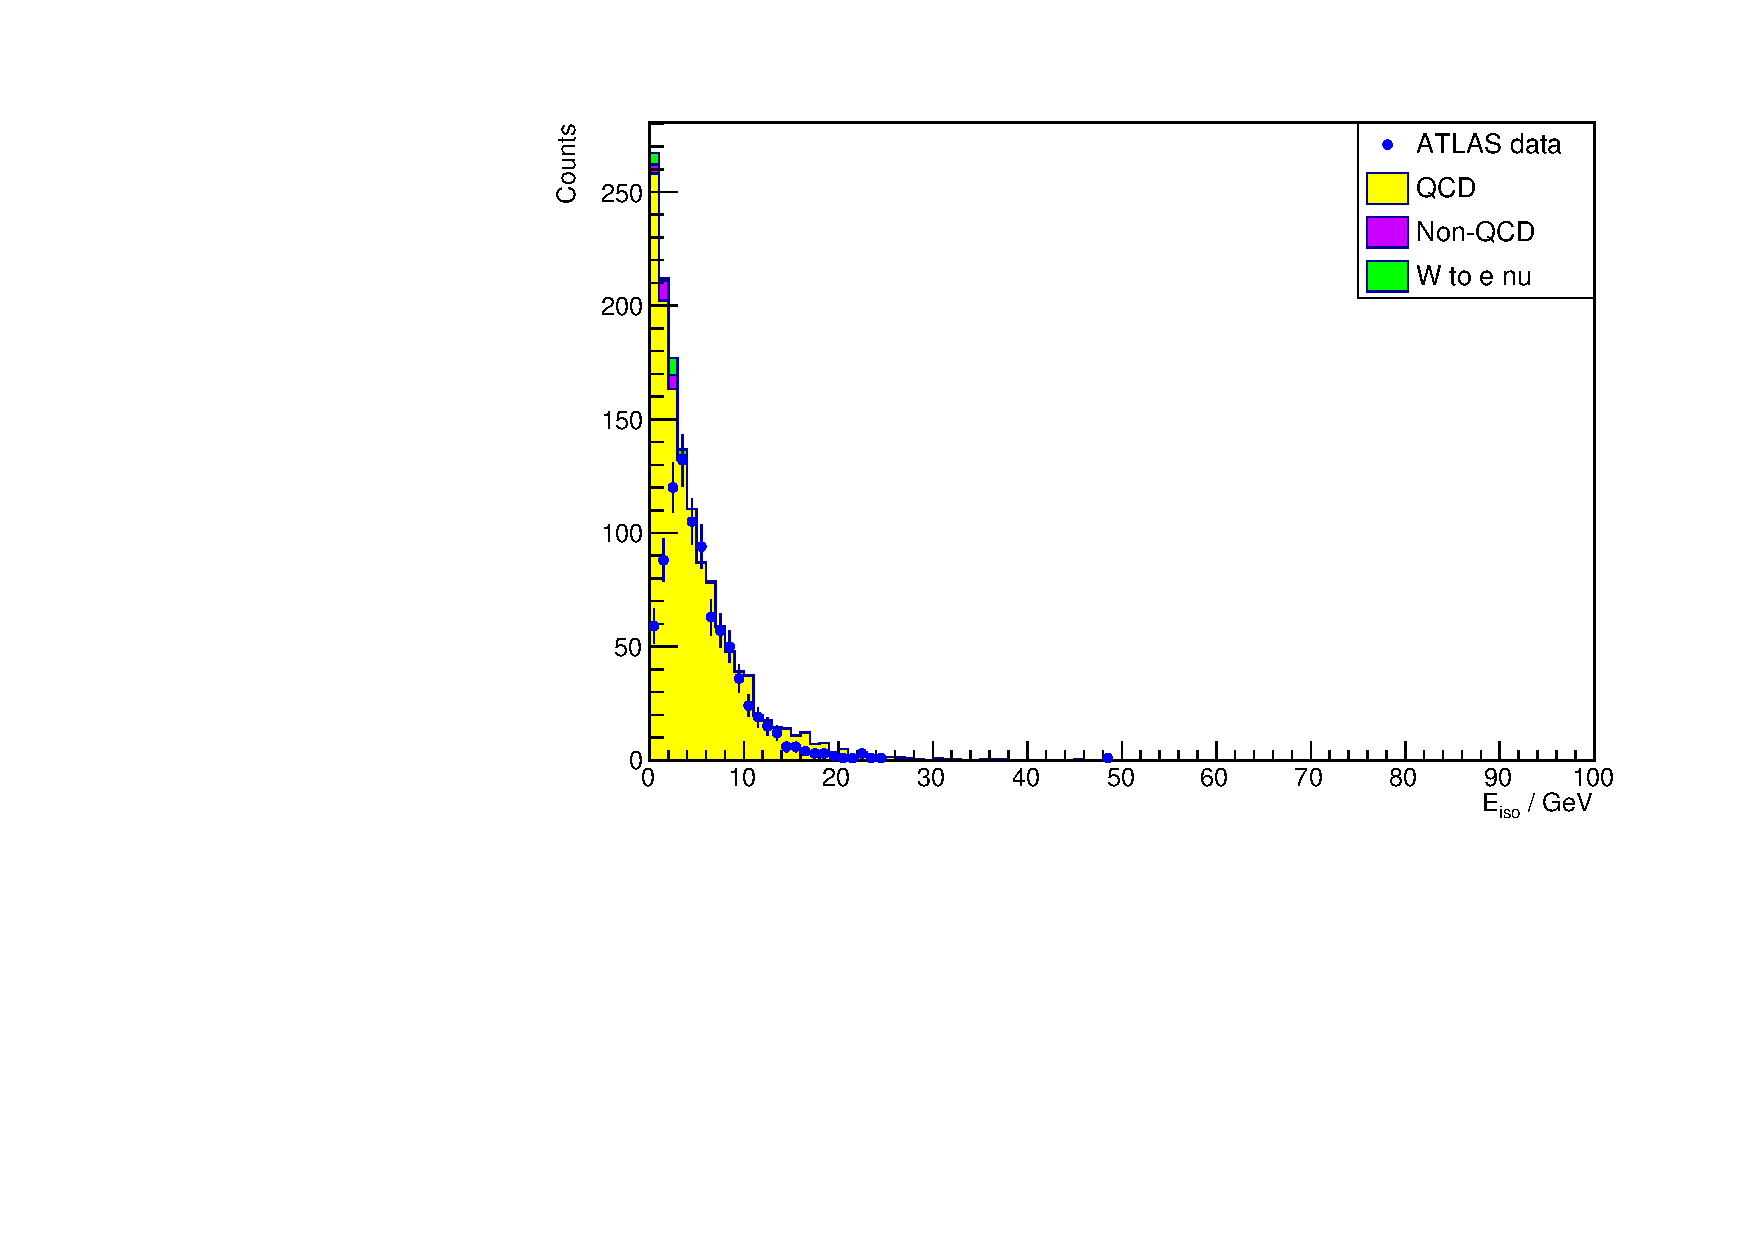
\includegraphics[width=\linewidth]{P1_pics/cuts/el_etiso_qcd_038.pdf}
		\caption{$E_t^{\text{iso}}$, QCD=$0.38$}
	\end{subfigure}
	\begin{subfigure}{0.49\linewidth}
		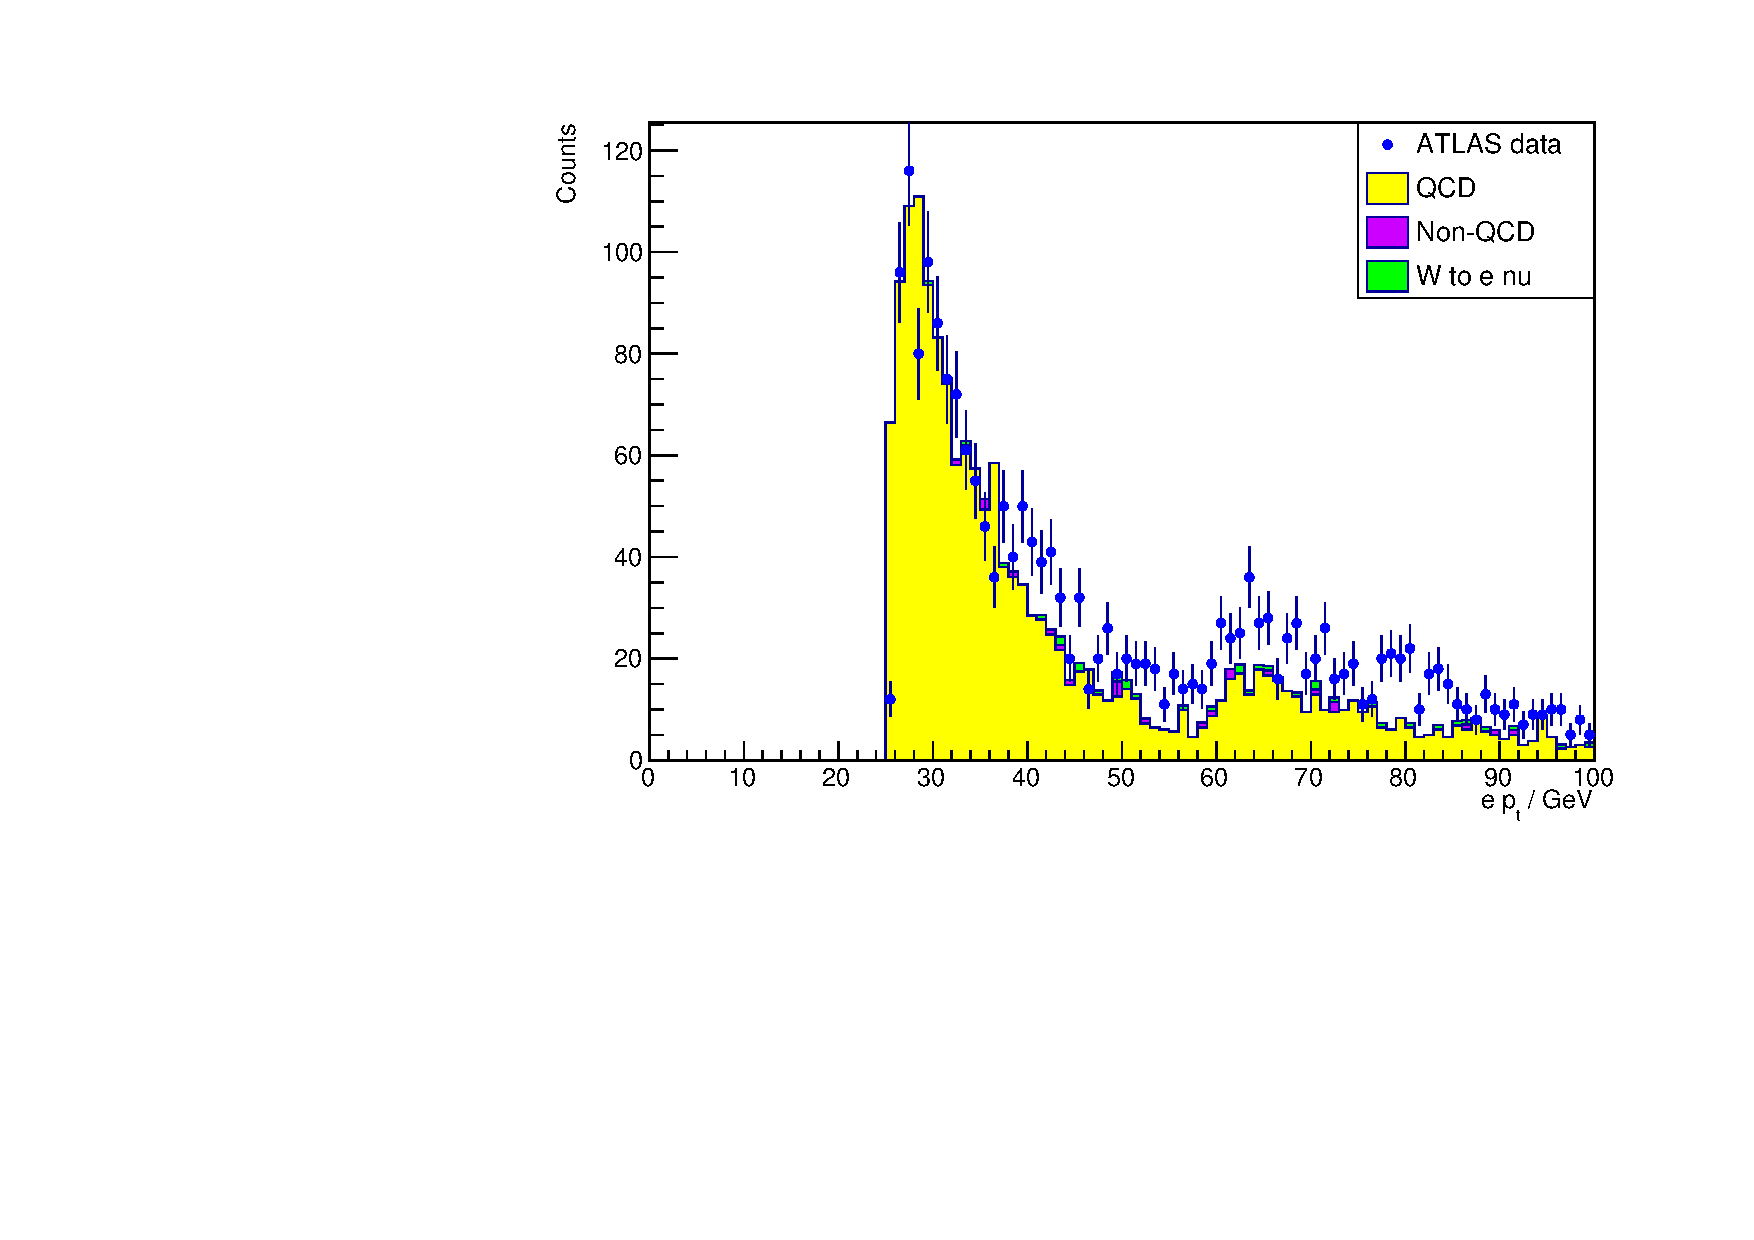
\includegraphics[width=\linewidth]{P1_pics/cuts/el_pt_qcd_038.pdf}
		\caption{$p_t^{\text{e}}$, QCD=$0.38$}
	\end{subfigure}
	\begin{subfigure}{0.49\linewidth}
		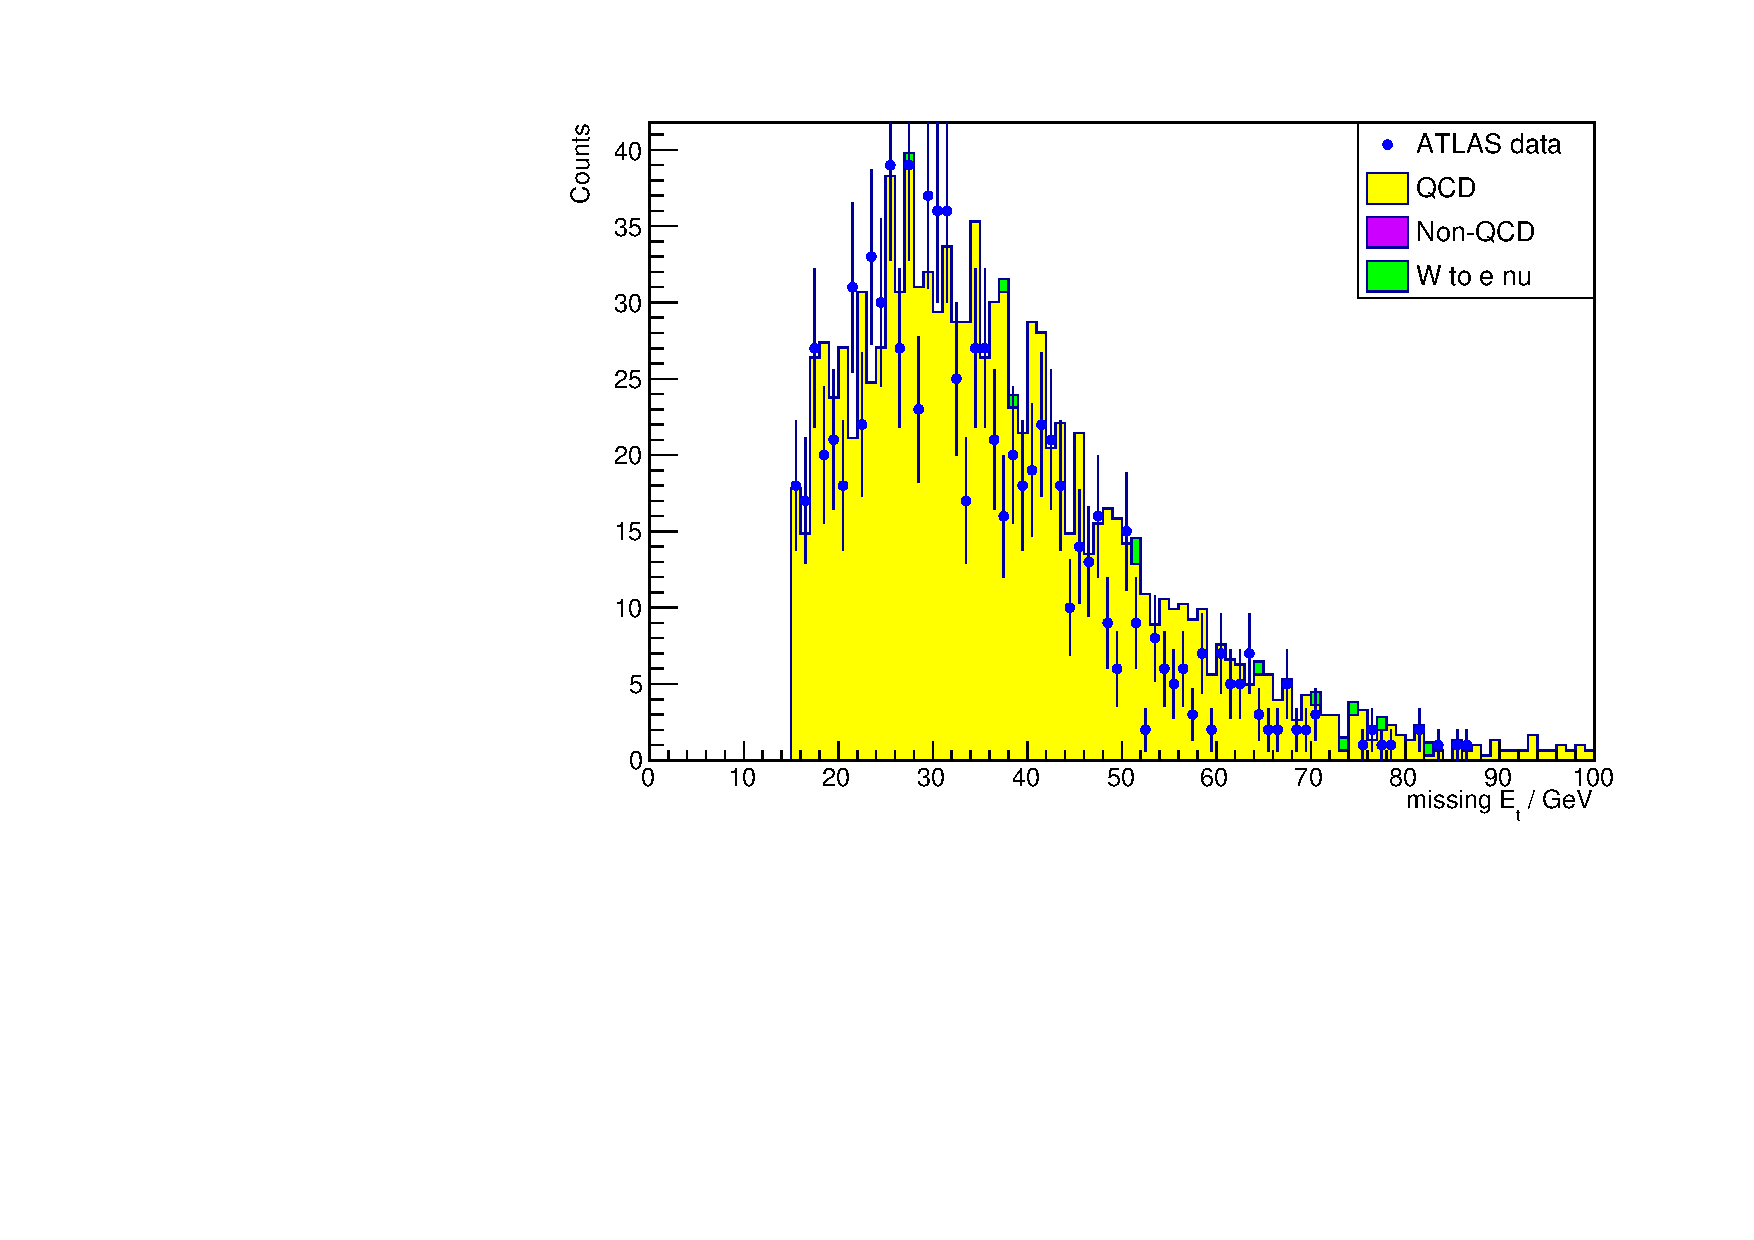
\includegraphics[width=\linewidth]{P1_pics/cuts/etmis_qcd_033.pdf}
		\caption{$\not$$E_t$, QCD=$0.33$}
	\end{subfigure}
	\begin{subfigure}{0.49\linewidth}
		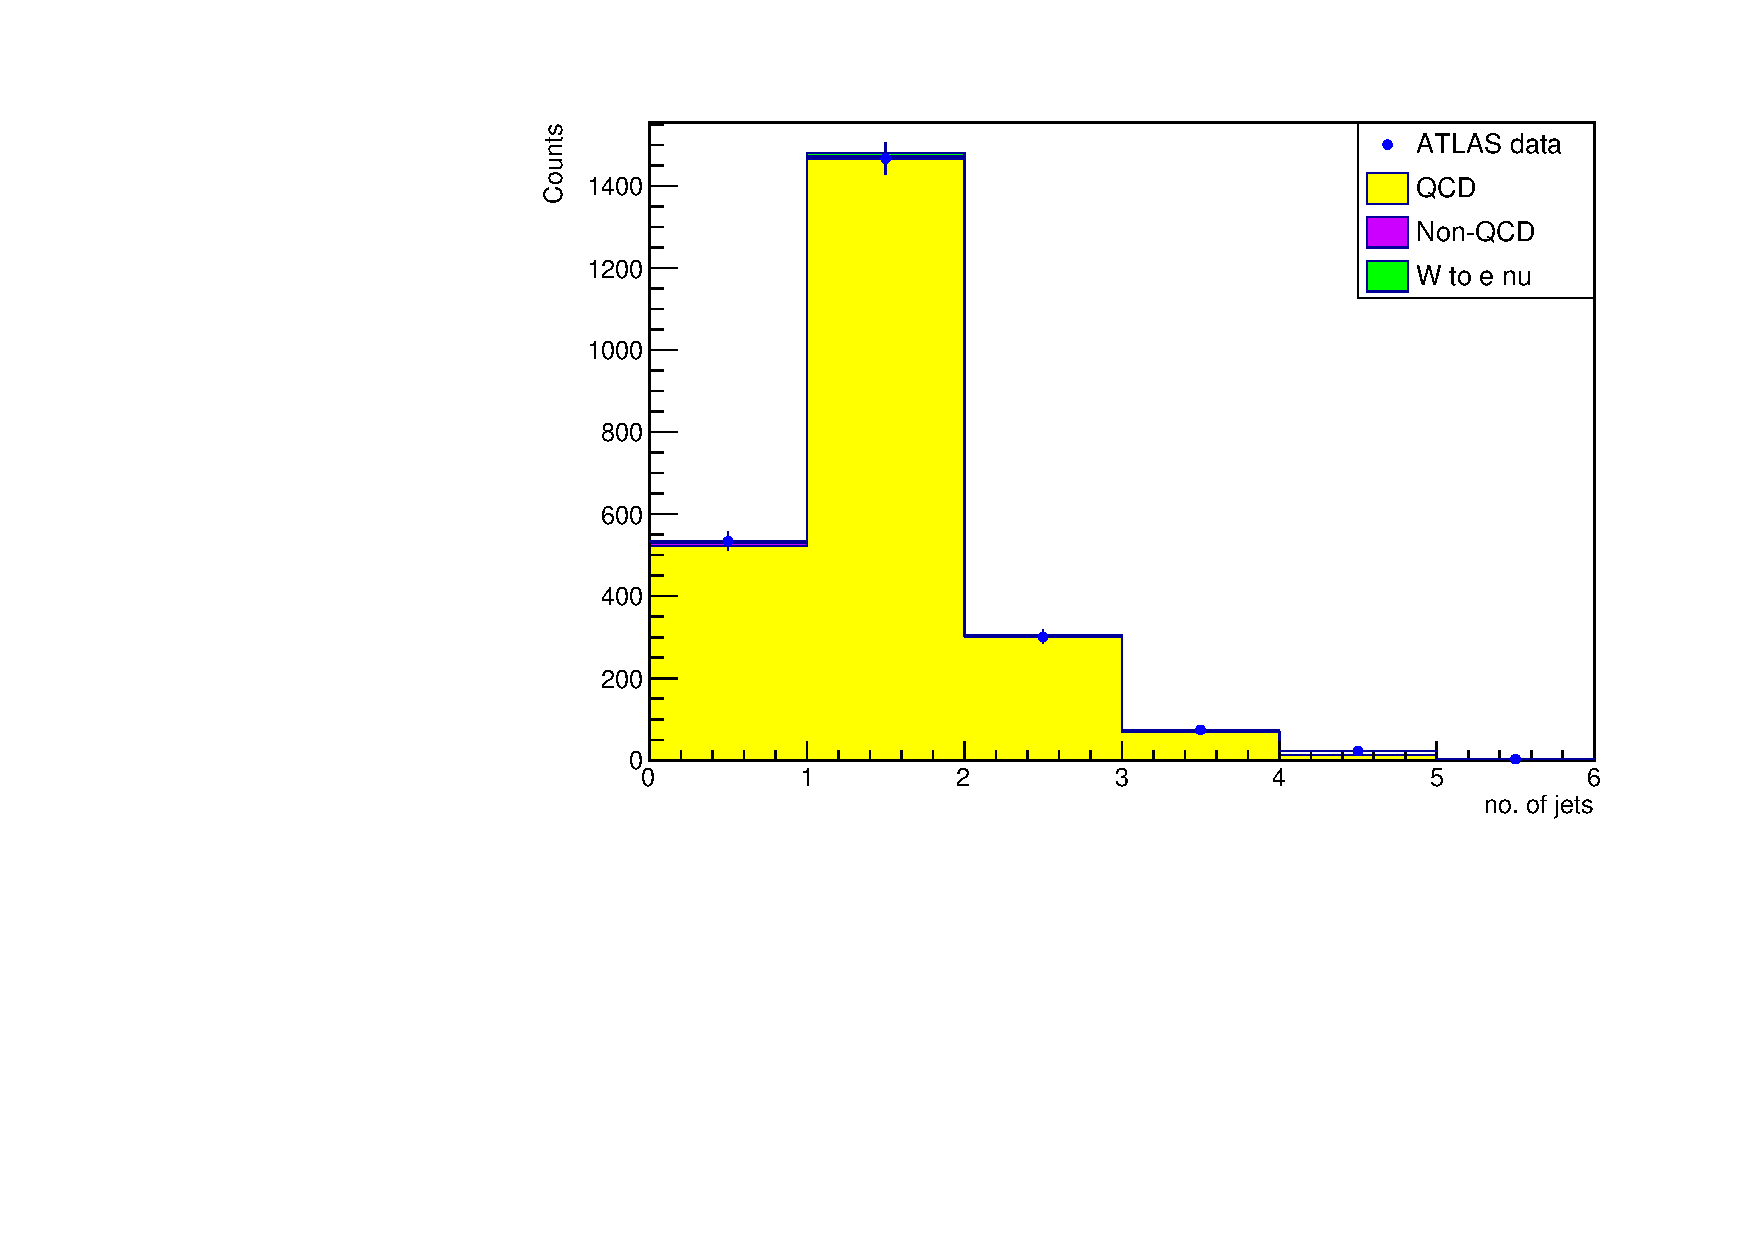
\includegraphics[width=\linewidth]{P1_pics/cuts/njet_qcd_031.pdf}
		\caption{$n_{\text{jet}}$, QCD=$0.31$}
	\end{subfigure}
	\begin{subfigure}{0.49\linewidth}
		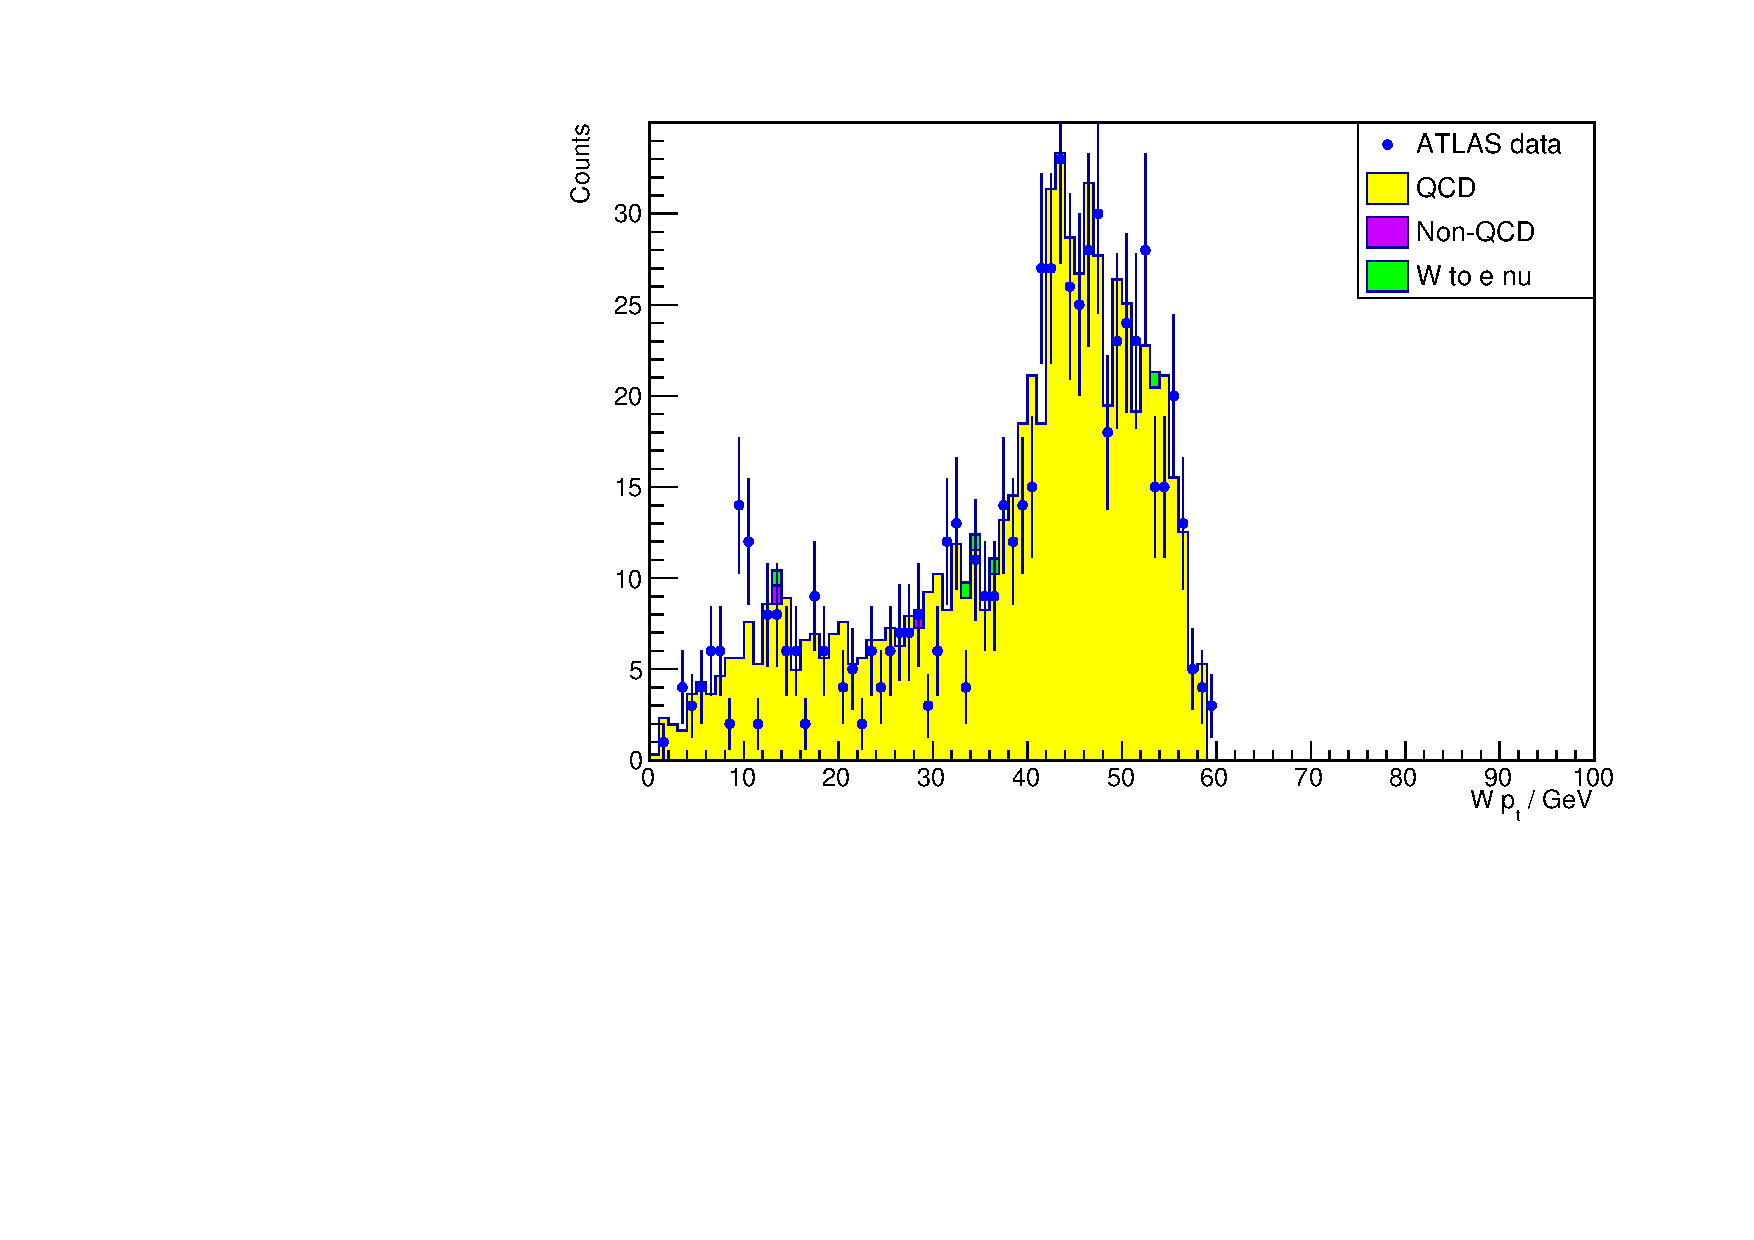
\includegraphics[width=\linewidth]{P1_pics/cuts/ptw_qcd_033.pdf}
		\caption{$p_{t}^W$, QCD=$0.33$}
	\end{subfigure}
	\caption{Inverse cut selection and applied QCD-scale factor for the different properties. ATLAS data (blue), simulated $Z\to ee$ decay events (green) and background (yellow) cuts are performed on every parameter save the one shown respectively}\label{fig:QCD}
\end{figure}

\begin{figure}[H]
	\vspace{-0.3cm}
	\centering
	\begin{subfigure}{\linewidth}
		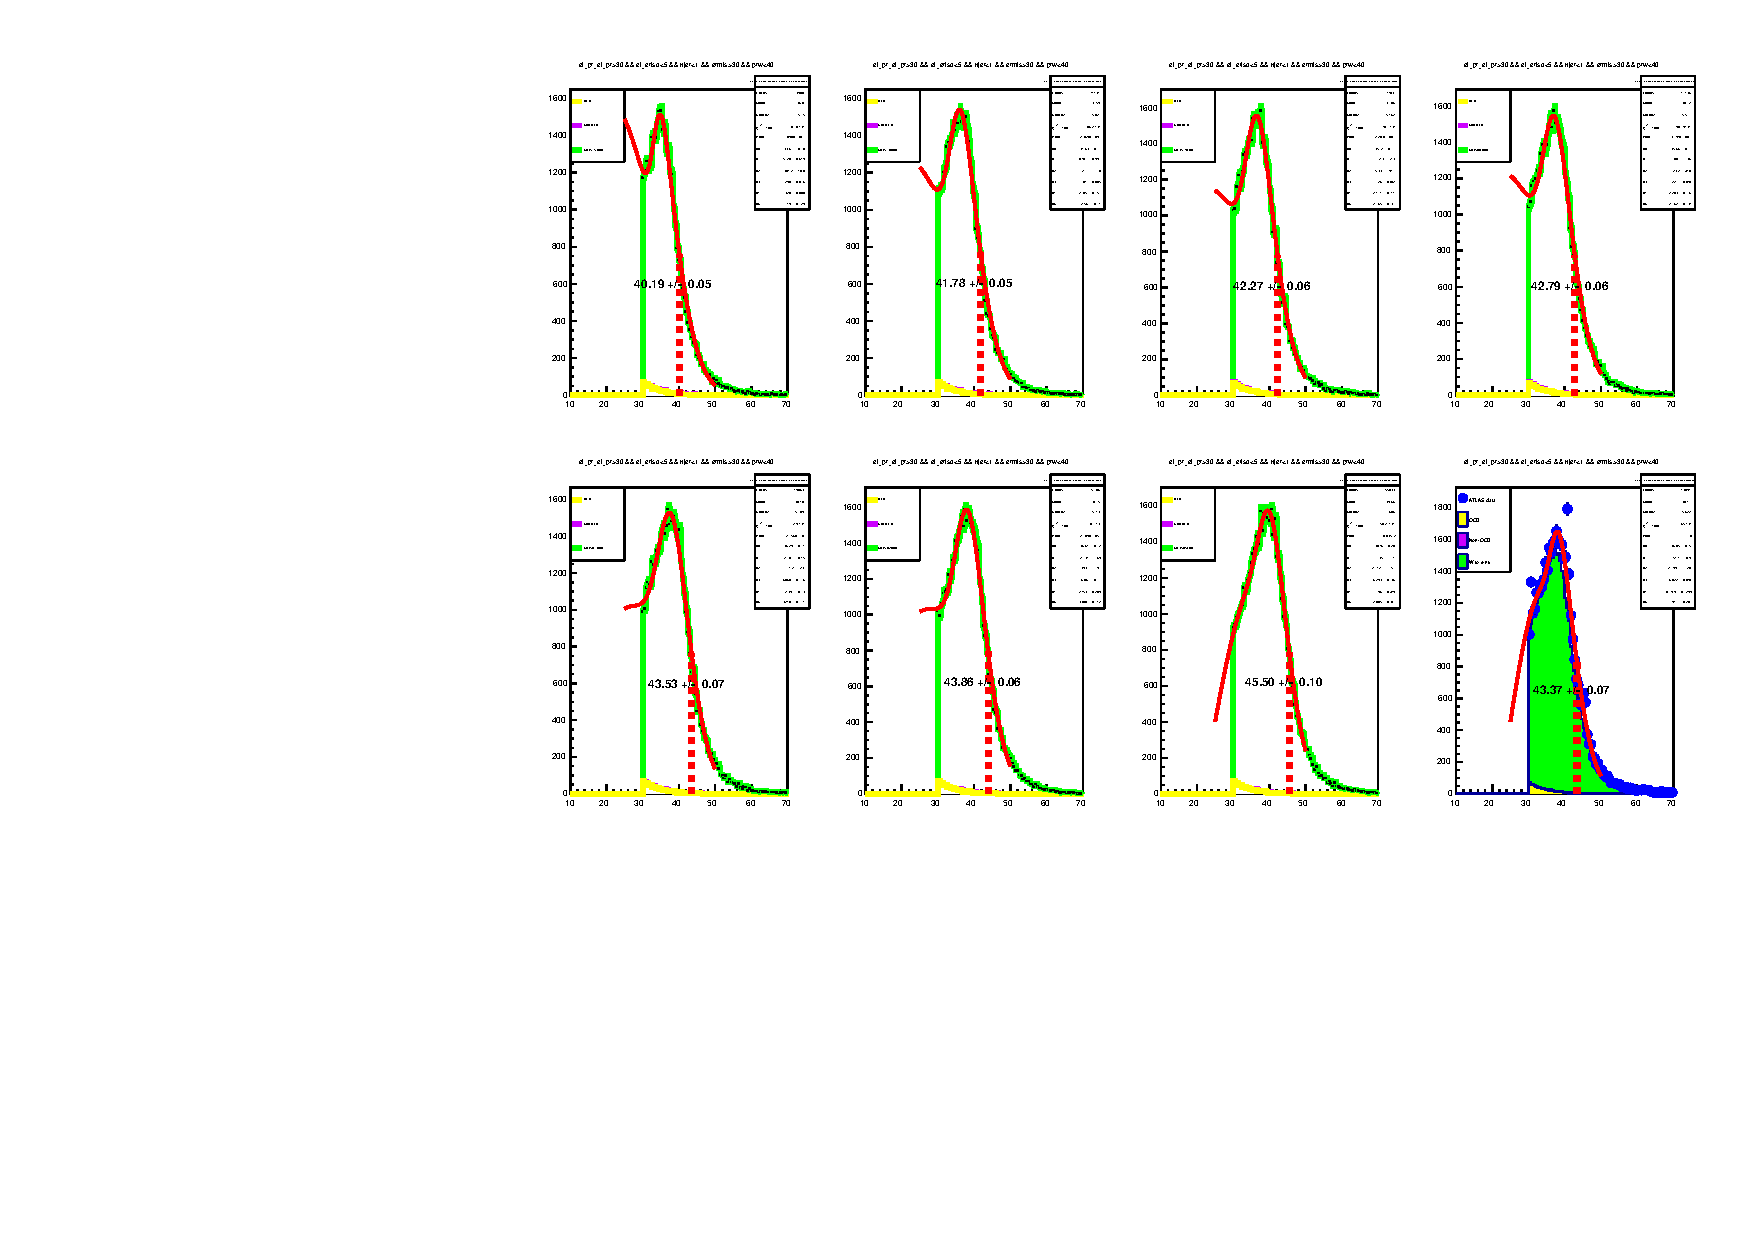
\includegraphics[width=\linewidth]{P1_pics/gauge/gauge_xmin_25_xmax_50.pdf}
		\caption{$x_\text{min}=25\text{GeV} \text{\phantom{ n } and \phantom{ n }} x_{\text{max}}=50\text{GeV}$}
	\end{subfigure}
	\begin{subfigure}{\linewidth}
		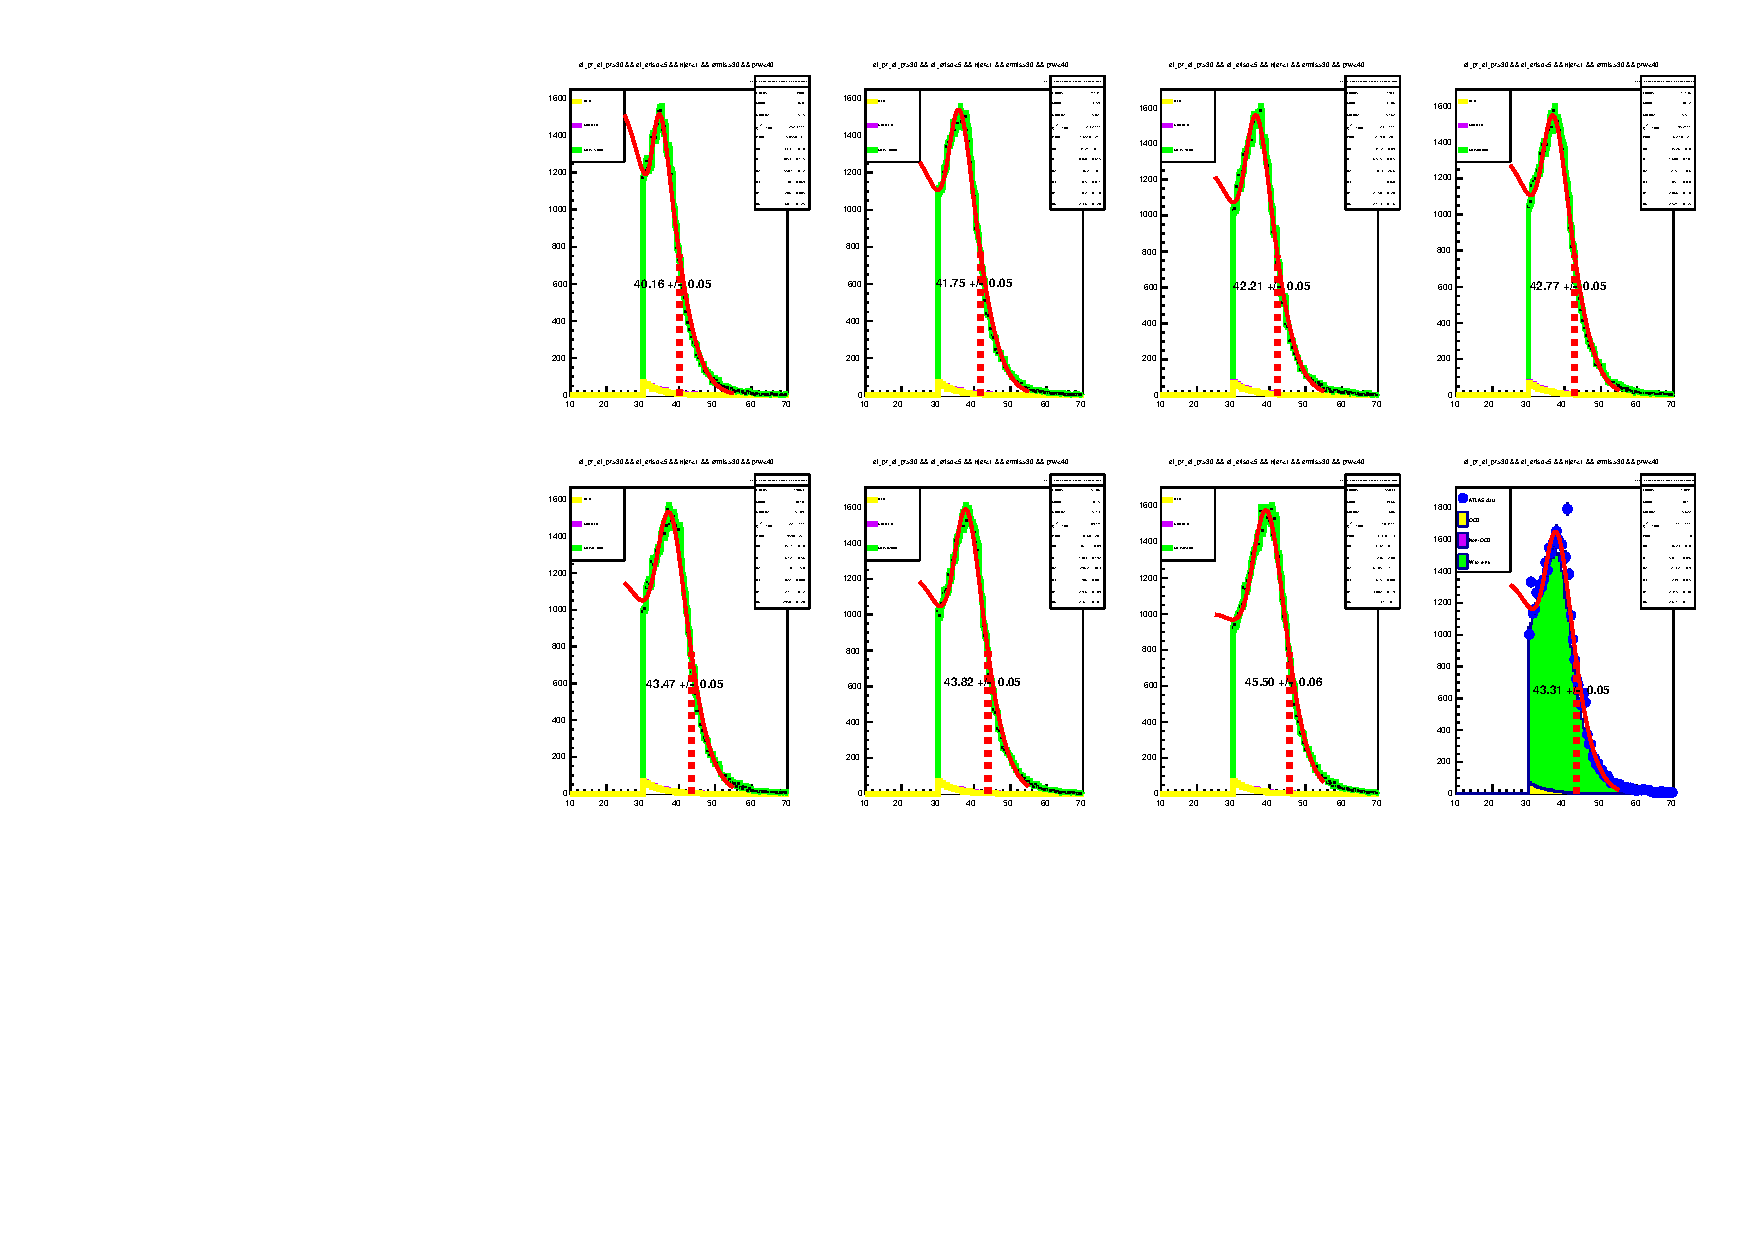
\includegraphics[width=\linewidth]{P1_pics/gauge/gauge_xmin_25_xmax_55.pdf}
		\caption{$x_\text{min}=25\text{GeV} \text{\phantom{ n } and \phantom{ n }} x_{\text{max}}=55\text{GeV}$}
	\end{subfigure}
	\caption{}
\end{figure}
\begin{figure}[H]\ContinuedFloat
	\centering
	\begin{subfigure}{\linewidth}
		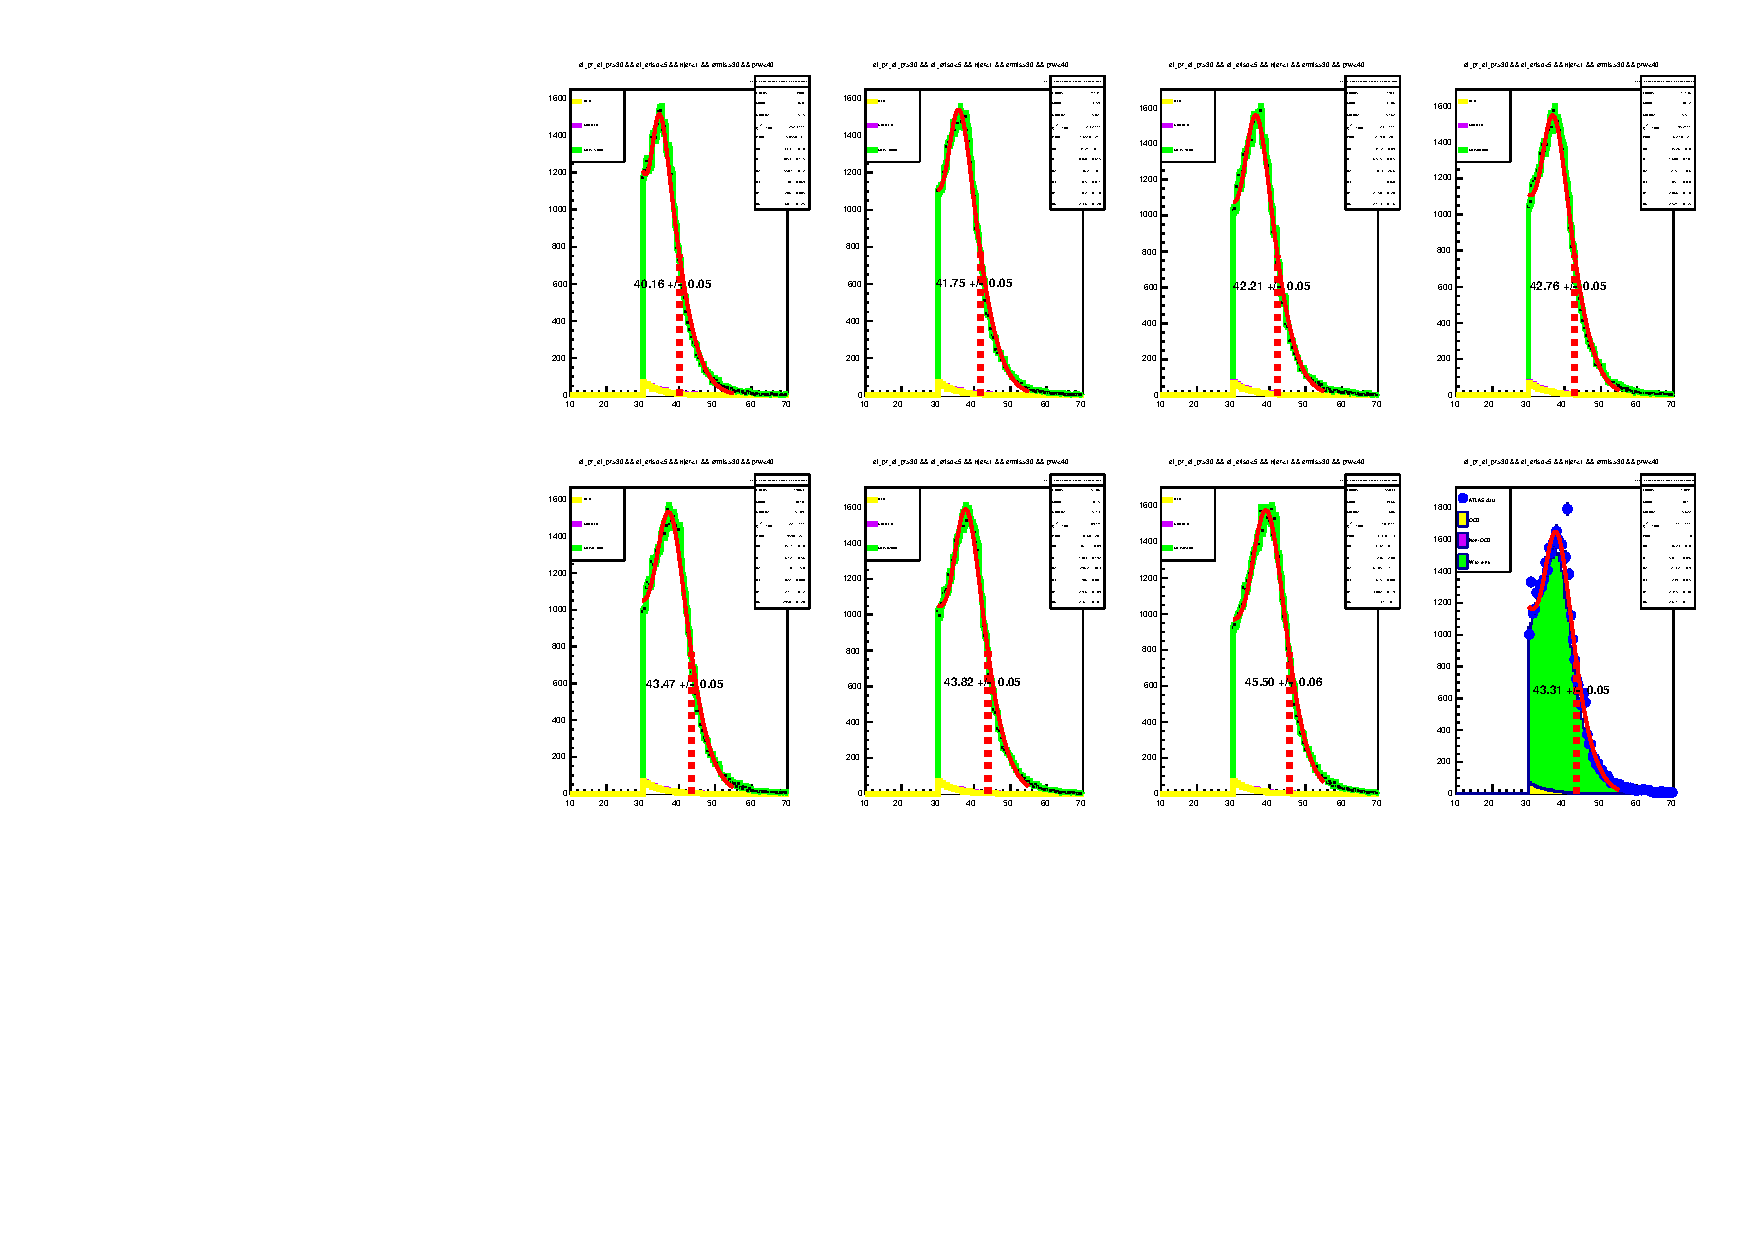
\includegraphics[width=\linewidth]{P1_pics/gauge/gauge_xmin_30_xmax_55.pdf}
		\caption{$x_\text{min}=30\text{GeV} \text{\phantom{ n } and \phantom{ n }} x_{\text{max}}=55\text{GeV}$}
	\end{subfigure}
	\caption{$p_T$ spectra (GeV) for the datasets: MCW75, MCW78, MCW79, MCW80, MCW81, MCW82, MCW85 and Wenu. The plot sets differ in the fit range $[x_\text{min}, x_\text{max}]$. For all datasets we applied the QCD-scale factor and cuts from section \ref{sec:cuts}.  x-axis: electron $p_t$, y-axis: no. of entries}\label{fig:boundaries}
\end{figure}
\vspace{-0.5cm}
\begin{figure}[H]
	\begin{subfigure}{0.49\linewidth}
		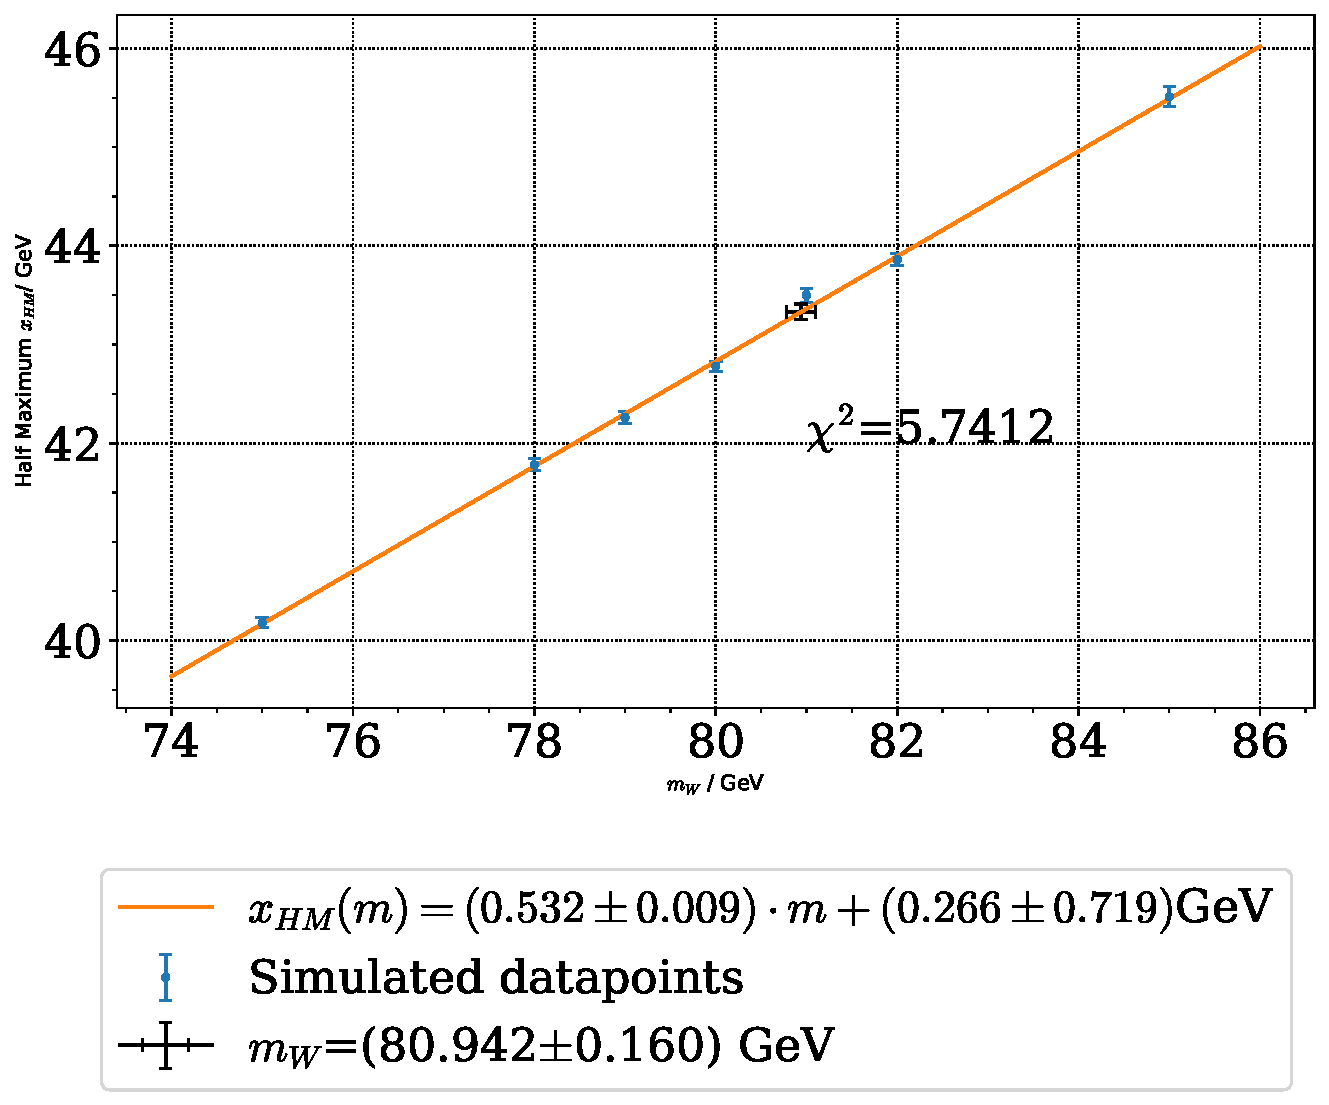
\includegraphics[width=\linewidth]{P1_pics/gauge_results/gauge_el_etiso_ll.pdf}
		\caption{$E_t^\text{iso}<5$ GeV}
	\end{subfigure}
	\begin{subfigure}{0.49\linewidth}
		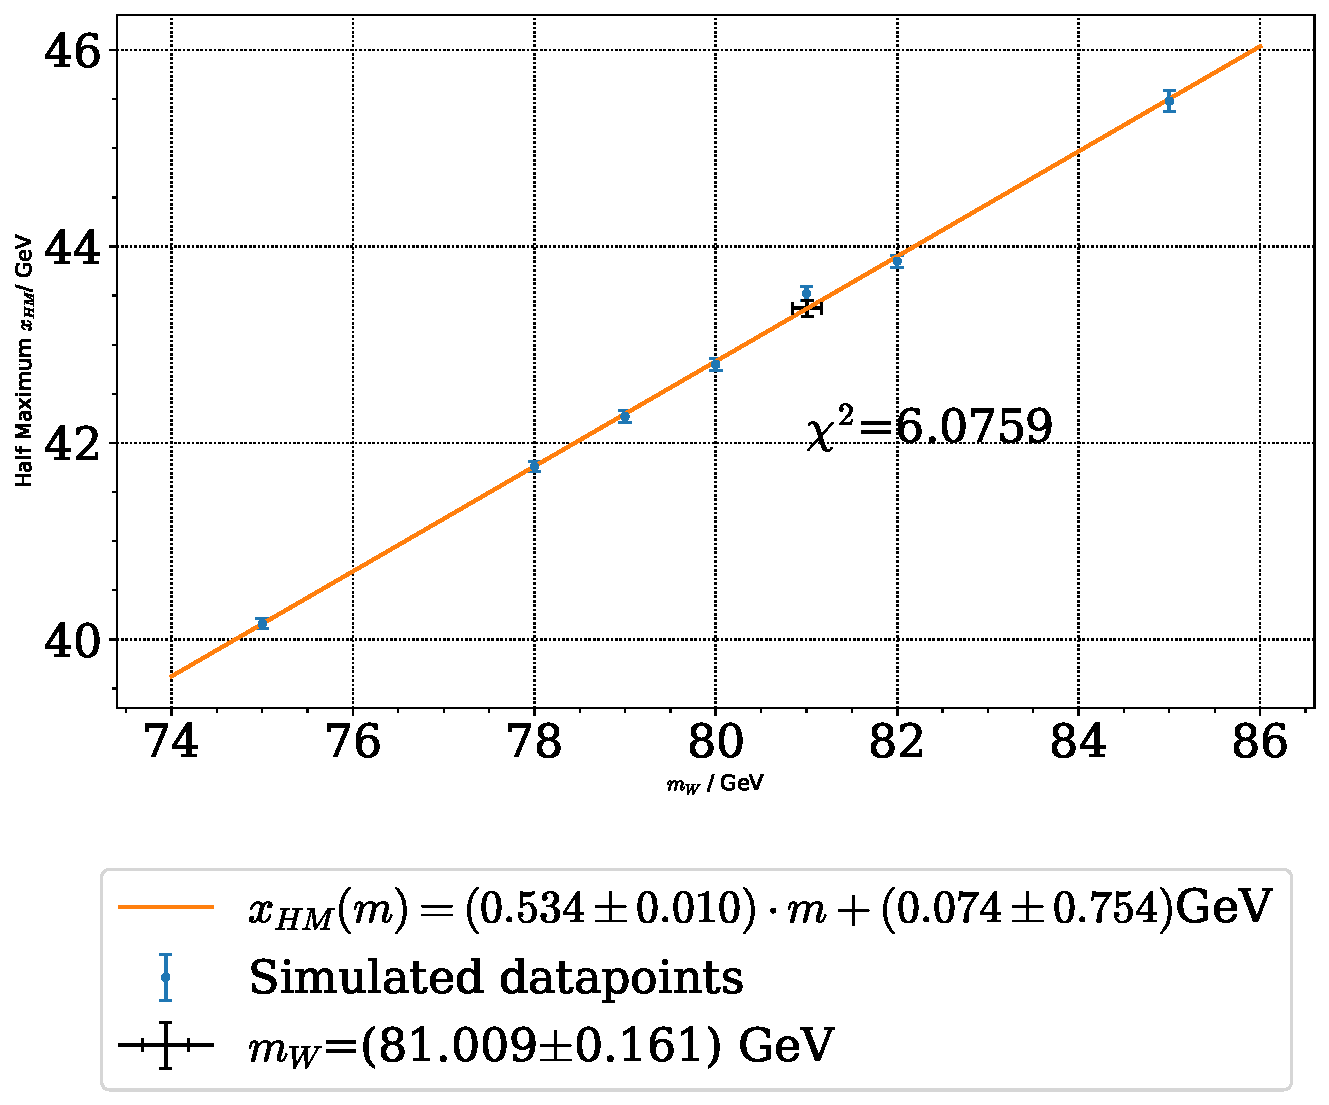
\includegraphics[width=\linewidth]{P1_pics/gauge_results/gauge_el_etiso_ul.pdf}
		\caption{$E_t^\text{iso}<7$ GeV}
	\end{subfigure}
	\caption{Gauge curves for varied parameters. All other parameters are fixed (table \ref{tab:cuts}).}
\end{figure}
\begin{figure}[H]\ContinuedFloat
	\begin{subfigure}{0.49\linewidth}
		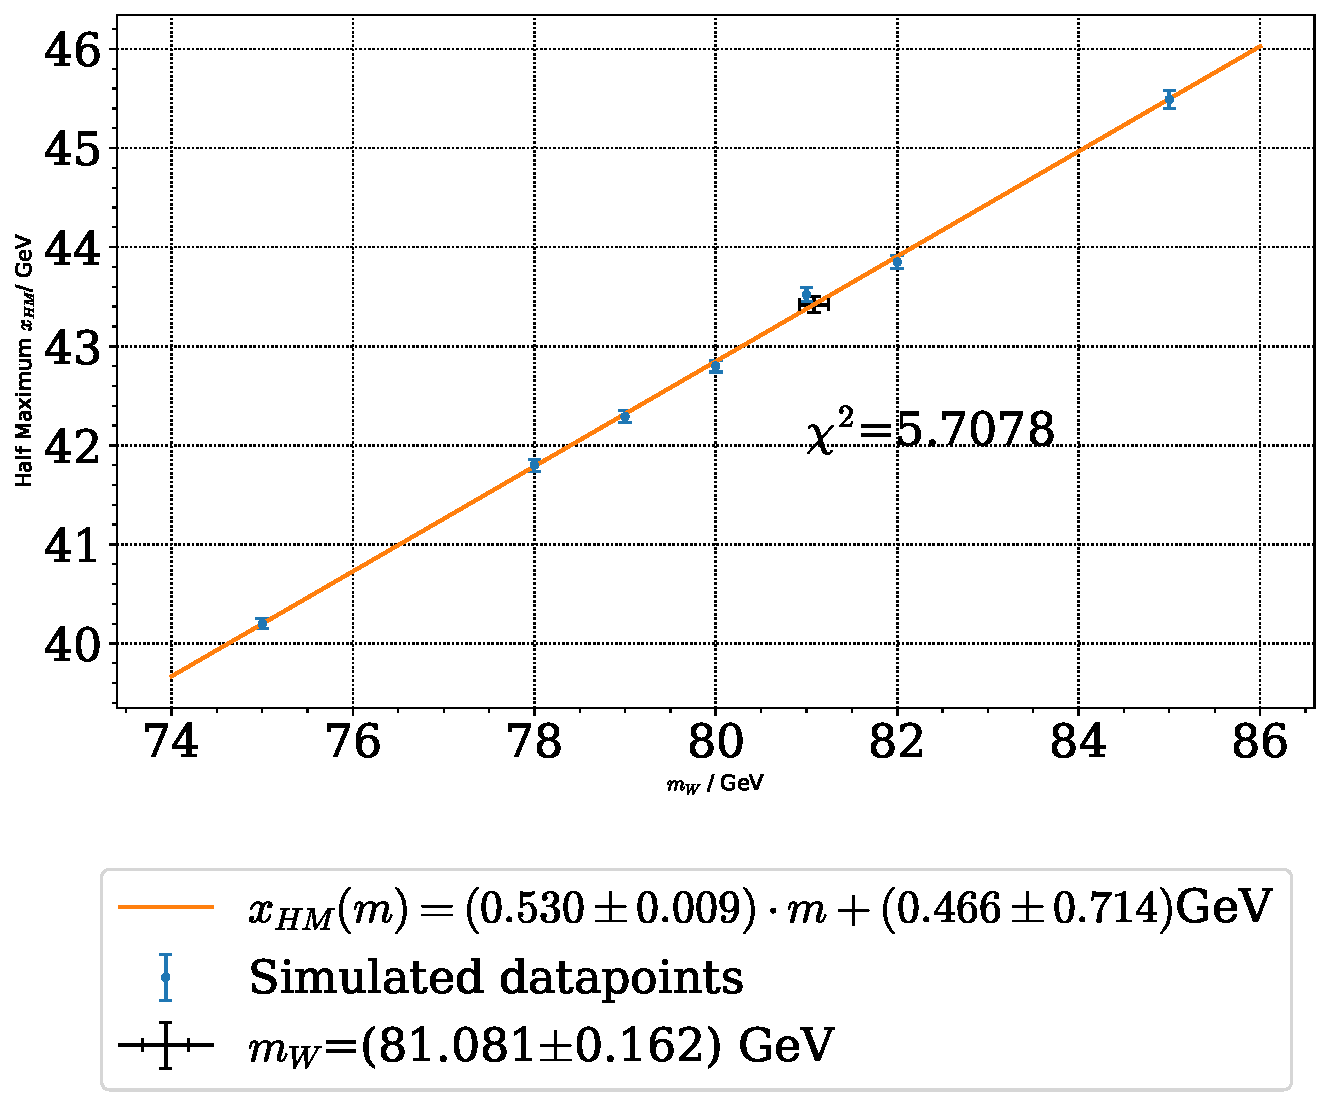
\includegraphics[width=\linewidth]{P1_pics/gauge_results/gauge_etimis_ll.pdf}
		\caption{$\not$$E_t>28$ GeV}
	\end{subfigure}
	\begin{subfigure}{0.49\linewidth}
		\includegraphics[width=\linewidth]{P1_pics/gauge_results/gauge_etmis_ul.pdf}
		\caption{$\not$$E_t>32$ GeV}
	\end{subfigure}
	\begin{subfigure}{0.49\linewidth}
		\includegraphics[width=\linewidth]{P1_pics/gauge_results/gauge_pt_ll.pdf}
		\caption{$p_t^e>28$ GeV}
	\end{subfigure}
	\begin{subfigure}{0.49\linewidth}
		\includegraphics[width=\linewidth]{P1_pics/gauge_results/gauge_pt_ul.pdf}
		\caption{$p_t^e>32$ GeV}
	\end{subfigure}
	\begin{subfigure}{0.49\linewidth}
		\includegraphics[width=\linewidth]{P1_pics/gauge_results/gauge_ptw_ll.pdf}
		\caption{$p_t^W<38$ GeV}
	\end{subfigure}
	\begin{subfigure}{0.49\linewidth}
		\includegraphics[width=\linewidth]{P1_pics/gauge_results/gauge_ptw_ul.pdf}
		\caption{$p_t^W<42$ GeV}
	\end{subfigure}
	\caption{Gauge curves for varied parameters (captions). All other parameters are fixed to the values of table \ref{tab:cuts}.}
\end{figure}
\begin{figure}[H]\ContinuedFloat
	\centering
	\begin{subfigure}{0.49\linewidth}
		\includegraphics[width=\linewidth]{P1_pics/gauge_results/gauge_qcd_std_ll.pdf}
		\caption{QCD-Scale factor$=0.317$}
	\end{subfigure}
	\begin{subfigure}{0.49\linewidth}
		\includegraphics[width=\linewidth]{P1_pics/gauge_results/gauge_qcd_std_ul.pdf}
		\caption{QCD-Scale factor$=0.375$}
	\end{subfigure}
	\begin{subfigure}{0.49\linewidth}
		\includegraphics[width=\linewidth]{P1_pics/gauge_results/gauge_xmin_25_xmax_50.pdf}
		\caption{$x_\text{min}=25 \text{GeV}, x_\text{max}=50\text{GeV}$}
	\end{subfigure}
	\begin{subfigure}{0.49\linewidth}
		\includegraphics[width=\linewidth]{P1_pics/gauge_results/gauge_xmin_25_xmax_55.pdf}
		\caption{$x_\text{min}=25\text{GeV}, x_\text{max}=55\text{GeV}$}
	\end{subfigure}
	\begin{subfigure}{0.49\linewidth}
		\includegraphics[width=\linewidth]{P1_pics/gauge_results/gauge_xmin_30_xmax_55.pdf}
		\caption{$x_\text{min}=30\text{GeV}, x_\text{max}=55\text{GeV}$}
	\end{subfigure}
	\caption{Gauge curves for varied parameters (captions). All other parameters are fixed to the values of table \ref{tab:cuts}.}\label{fig:gauge_curve_rest}
\end{figure}
\newpage


\printbibliography[heading=bibintoc]
\end{document}
